% Options for packages loaded elsewhere
\PassOptionsToPackage{unicode}{hyperref}
\PassOptionsToPackage{hyphens}{url}
%
\documentclass[
  openany]{book}
\usepackage{amsmath,amssymb}
\usepackage{iftex}
\ifPDFTeX
  \usepackage[T1]{fontenc}
  \usepackage[utf8]{inputenc}
  \usepackage{textcomp} % provide euro and other symbols
\else % if luatex or xetex
  \usepackage{unicode-math} % this also loads fontspec
  \defaultfontfeatures{Scale=MatchLowercase}
  \defaultfontfeatures[\rmfamily]{Ligatures=TeX,Scale=1}
\fi
\usepackage{lmodern}
\ifPDFTeX\else
  % xetex/luatex font selection
\fi
% Use upquote if available, for straight quotes in verbatim environments
\IfFileExists{upquote.sty}{\usepackage{upquote}}{}
\IfFileExists{microtype.sty}{% use microtype if available
  \usepackage[]{microtype}
  \UseMicrotypeSet[protrusion]{basicmath} % disable protrusion for tt fonts
}{}
\makeatletter
\@ifundefined{KOMAClassName}{% if non-KOMA class
  \IfFileExists{parskip.sty}{%
    \usepackage{parskip}
  }{% else
    \setlength{\parindent}{0pt}
    \setlength{\parskip}{6pt plus 2pt minus 1pt}}
}{% if KOMA class
  \KOMAoptions{parskip=half}}
\makeatother
\usepackage{xcolor}
\usepackage{color}
\usepackage{fancyvrb}
\newcommand{\VerbBar}{|}
\newcommand{\VERB}{\Verb[commandchars=\\\{\}]}
\DefineVerbatimEnvironment{Highlighting}{Verbatim}{commandchars=\\\{\}}
% Add ',fontsize=\small' for more characters per line
\usepackage{framed}
\definecolor{shadecolor}{RGB}{248,248,248}
\newenvironment{Shaded}{\begin{snugshade}}{\end{snugshade}}
\newcommand{\AlertTok}[1]{\textcolor[rgb]{0.94,0.16,0.16}{#1}}
\newcommand{\AnnotationTok}[1]{\textcolor[rgb]{0.56,0.35,0.01}{\textbf{\textit{#1}}}}
\newcommand{\AttributeTok}[1]{\textcolor[rgb]{0.13,0.29,0.53}{#1}}
\newcommand{\BaseNTok}[1]{\textcolor[rgb]{0.00,0.00,0.81}{#1}}
\newcommand{\BuiltInTok}[1]{#1}
\newcommand{\CharTok}[1]{\textcolor[rgb]{0.31,0.60,0.02}{#1}}
\newcommand{\CommentTok}[1]{\textcolor[rgb]{0.56,0.35,0.01}{\textit{#1}}}
\newcommand{\CommentVarTok}[1]{\textcolor[rgb]{0.56,0.35,0.01}{\textbf{\textit{#1}}}}
\newcommand{\ConstantTok}[1]{\textcolor[rgb]{0.56,0.35,0.01}{#1}}
\newcommand{\ControlFlowTok}[1]{\textcolor[rgb]{0.13,0.29,0.53}{\textbf{#1}}}
\newcommand{\DataTypeTok}[1]{\textcolor[rgb]{0.13,0.29,0.53}{#1}}
\newcommand{\DecValTok}[1]{\textcolor[rgb]{0.00,0.00,0.81}{#1}}
\newcommand{\DocumentationTok}[1]{\textcolor[rgb]{0.56,0.35,0.01}{\textbf{\textit{#1}}}}
\newcommand{\ErrorTok}[1]{\textcolor[rgb]{0.64,0.00,0.00}{\textbf{#1}}}
\newcommand{\ExtensionTok}[1]{#1}
\newcommand{\FloatTok}[1]{\textcolor[rgb]{0.00,0.00,0.81}{#1}}
\newcommand{\FunctionTok}[1]{\textcolor[rgb]{0.13,0.29,0.53}{\textbf{#1}}}
\newcommand{\ImportTok}[1]{#1}
\newcommand{\InformationTok}[1]{\textcolor[rgb]{0.56,0.35,0.01}{\textbf{\textit{#1}}}}
\newcommand{\KeywordTok}[1]{\textcolor[rgb]{0.13,0.29,0.53}{\textbf{#1}}}
\newcommand{\NormalTok}[1]{#1}
\newcommand{\OperatorTok}[1]{\textcolor[rgb]{0.81,0.36,0.00}{\textbf{#1}}}
\newcommand{\OtherTok}[1]{\textcolor[rgb]{0.56,0.35,0.01}{#1}}
\newcommand{\PreprocessorTok}[1]{\textcolor[rgb]{0.56,0.35,0.01}{\textit{#1}}}
\newcommand{\RegionMarkerTok}[1]{#1}
\newcommand{\SpecialCharTok}[1]{\textcolor[rgb]{0.81,0.36,0.00}{\textbf{#1}}}
\newcommand{\SpecialStringTok}[1]{\textcolor[rgb]{0.31,0.60,0.02}{#1}}
\newcommand{\StringTok}[1]{\textcolor[rgb]{0.31,0.60,0.02}{#1}}
\newcommand{\VariableTok}[1]{\textcolor[rgb]{0.00,0.00,0.00}{#1}}
\newcommand{\VerbatimStringTok}[1]{\textcolor[rgb]{0.31,0.60,0.02}{#1}}
\newcommand{\WarningTok}[1]{\textcolor[rgb]{0.56,0.35,0.01}{\textbf{\textit{#1}}}}
\usepackage{longtable,booktabs,array}
\usepackage{calc} % for calculating minipage widths
% Correct order of tables after \paragraph or \subparagraph
\usepackage{etoolbox}
\makeatletter
\patchcmd\longtable{\par}{\if@noskipsec\mbox{}\fi\par}{}{}
\makeatother
% Allow footnotes in longtable head/foot
\IfFileExists{footnotehyper.sty}{\usepackage{footnotehyper}}{\usepackage{footnote}}
\makesavenoteenv{longtable}
\usepackage{graphicx}
\makeatletter
\def\maxwidth{\ifdim\Gin@nat@width>\linewidth\linewidth\else\Gin@nat@width\fi}
\def\maxheight{\ifdim\Gin@nat@height>\textheight\textheight\else\Gin@nat@height\fi}
\makeatother
% Scale images if necessary, so that they will not overflow the page
% margins by default, and it is still possible to overwrite the defaults
% using explicit options in \includegraphics[width, height, ...]{}
\setkeys{Gin}{width=\maxwidth,height=\maxheight,keepaspectratio}
% Set default figure placement to htbp
\makeatletter
\def\fps@figure{htbp}
\makeatother
\setlength{\emergencystretch}{3em} % prevent overfull lines
\providecommand{\tightlist}{%
  \setlength{\itemsep}{0pt}\setlength{\parskip}{0pt}}
\setcounter{secnumdepth}{5}
\usepackage[margin = 1in]{geometry}
\usepackage[breaklinks=true]{hyperref}
\ifLuaTeX
  \usepackage{selnolig}  % disable illegal ligatures
\fi
\usepackage[]{natbib}
\bibliographystyle{apalike}
\IfFileExists{bookmark.sty}{\usepackage{bookmark}}{\usepackage{hyperref}}
\IfFileExists{xurl.sty}{\usepackage{xurl}}{} % add URL line breaks if available
\urlstyle{same}
\hypersetup{
  pdftitle={Clinical Trials 4H},
  pdfauthor={Rachel Oughton},
  hidelinks,
  pdfcreator={LaTeX via pandoc}}

\title{Clinical Trials 4H}
\author{Rachel Oughton}
\date{2024-02-04}

\usepackage{amsthm}
\newtheorem{theorem}{Theorem}[chapter]
\newtheorem{lemma}{Lemma}[chapter]
\newtheorem{corollary}{Corollary}[chapter]
\newtheorem{proposition}{Proposition}[chapter]
\newtheorem{conjecture}{Conjecture}[chapter]
\theoremstyle{definition}
\newtheorem{definition}{Definition}[chapter]
\theoremstyle{definition}
\newtheorem{example}{Example}[chapter]
\theoremstyle{definition}
\newtheorem{exercise}{Exercise}[chapter]
\theoremstyle{definition}
\newtheorem{hypothesis}{Hypothesis}[chapter]
\theoremstyle{remark}
\newtheorem*{remark}{Remark}
\newtheorem*{solution}{Solution}
\begin{document}
\maketitle

{
\setcounter{tocdepth}{1}
\tableofcontents
}
\hypertarget{welcome-to-clinical-trials-4h}{%
\chapter*{Welcome to Clinical Trials 4H!}\label{welcome-to-clinical-trials-4h}}
\addcontentsline{toc}{chapter}{Welcome to Clinical Trials 4H!}

This page contains the notes for Clinical Trials IV. As we progress through the course, more will appear. You can also download the PDF version (see the icon at the top left). If you notice any typos, mistakes or places that are unclear, please do let me know!

\hypertarget{practical-details}{%
\section*{Practical details}\label{practical-details}}
\addcontentsline{toc}{section}{Practical details}

\hypertarget{lectures}{%
\subsection*{Lectures}\label{lectures}}
\addcontentsline{toc}{subsection}{Lectures}

Our lectures are 12 noon on Mondays and 9am on Wednesdays, all in ES231. This is in the Earth Sciences / Arthur Holmes building, which is behind (almost surrounding) the Calman Learning Centre. The door of this room is actually labelled `Teaching Room 4'.

\hypertarget{computer-classes}{%
\subsection*{Computer classes}\label{computer-classes}}
\addcontentsline{toc}{subsection}{Computer classes}

We have two 2-hour practicals for this module. They are 11am - 1pm on the Fridays of weeks 14 and 19 (2nd February and 8th March). These classes are in RH-0003. This is Rowan House, which is in Upper Mountjoy, across the pond from the MCS building.

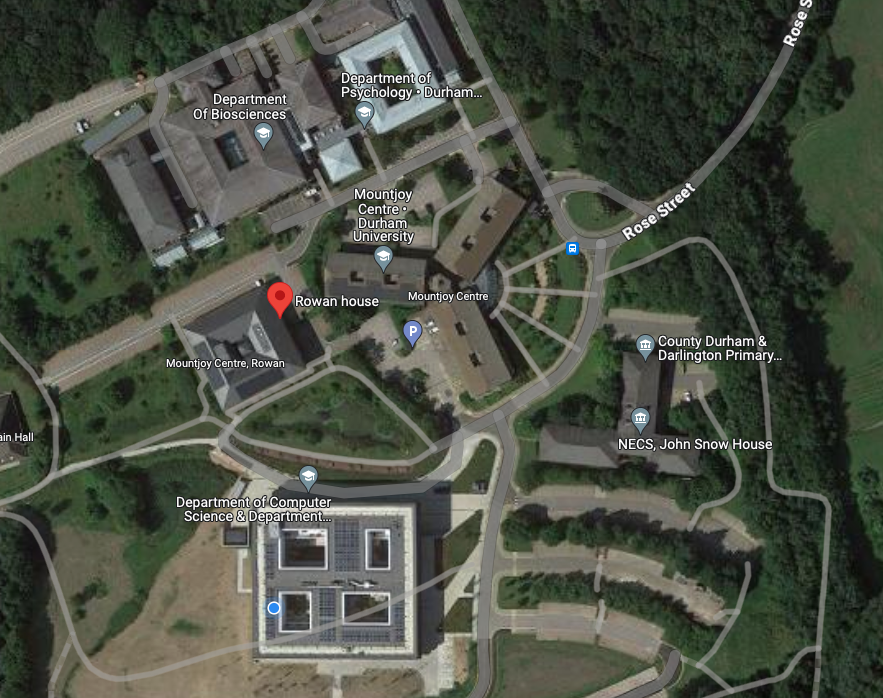
\includegraphics{images/rowanhouse_map.png}

\hypertarget{office-hour}{%
\subsection*{Office Hour}\label{office-hour}}
\addcontentsline{toc}{subsection}{Office Hour}

The office hour will be every Monday, 3-4pm, in MCS 2091 (this is a meeting room, not my office). If you walk up the stairs, keep straight on past the main maths office and computer room (MCS 2094), turn right and it's on your right through the double doors. Alternatively there are maps in the main areas!

\hypertarget{assessment}{%
\subsection*{Assessment}\label{assessment}}
\addcontentsline{toc}{subsection}{Assessment}

This module is assessed through two equally weighted pieces of coursework. The first will be assigned on Wednesday 7th February, the second on Wednesday 13th March.

There will also be some formative assignments throughout the course. More details on these to follow.

\hypertarget{books}{%
\subsection*{Books}\label{books}}
\addcontentsline{toc}{subsection}{Books}

The main reference for the first half of the course is \citet{matthews2006introduction}. There are a couple of copies in the Bill Bryson Library. Some other books we will make use of are \citet{hulley2013designing}, \citet{hayes2017cluster}. You shouldn't need to use any of these books, but of course you're welcome to if you want to read further.

\hypertarget{what-to-expect-from-this-module}{%
\section*{What to expect from this module}\label{what-to-expect-from-this-module}}
\addcontentsline{toc}{section}{What to expect from this module}

Clinical Trials IV is somewhat different from the majority of statistics modules, because

\begin{itemize}
\tightlist
\item
  It is more focussed on application than on methodology
\item
  It is assessed purely through coursework.
\end{itemize}

This means that your experience of it might be different from what you're used to

\begin{itemize}
\tightlist
\item
  We will cover quite a lot of different statistical methods (drawing on most of the 1H and 2H courses, and some 3H!) but not in great depth
\item
  There is no pressure to memorize anything - indeed, if you really were a trial statistician, you would definitely have access to the internet, various textbooks and even these notes (should they prove useful!).
\item
  There is an emphasis on understanding which method we use and why, and what it means. Hopefully this has been the case in some of your other modules too!
\end{itemize}

\hypertarget{what-i-expect-from-you}{%
\subsection*{What I expect from you}\label{what-i-expect-from-you}}
\addcontentsline{toc}{subsection}{What I expect from you}

Because we will be covering quite a lot of different areas within statistics, there may be some things that you haven't seen before (or can't remember very well). I will try my best to explain them as clearly as I can, but there isn't time to go into the nuts and bolts of everything we come across. Therefore, if you do feel a bit rusty on some area, you may need to read up on that a bit, so that you're happy with it. I am very happy to suggest resources from time to time, and you're welcome to come to the office hour to talk about such things.

This is the first year this course is running, and so I would also really appreciate your feedback. I may not be able to address everything (or I may only be able to implement things for following years), but if I can act on it quickly then I will!

\hypertarget{rct-intro}{%
\chapter{Introduction to Clinical Trials}\label{rct-intro}}

A clinical trial is an experiment, usually performed on human subjects, to test the effect of some sort of treatment or intervention. We may also use the term \textbf{Randomised controlled trial} (RCT). These are not fully the same thing; a clinical trial may not have been randomised, for example if it follows a pre-determined cohort through some sort of process. Likewise, an RCT may not be clinical, but instead may be about an intervention in some other setting like agriculture or education. For this module, we are really focussing on RCTs, and almost all of our examples will be clinical.

For the purposes of this module, a clinical trial will have two groups:

\begin{enumerate}
\def\labelenumi{\arabic{enumi}.}
\tightlist
\item
  The \textbf{treatment group} or \textbf{intervention group}: this group of people will be subject to the new treatment.
\item
  The \textbf{control group}: this group of people will be subject to the status quo - the `standard' or most widely used treatment path for their cohort (sometimes this is no treatment).
\end{enumerate}

These groups are usually, though not always, of the same size. Which group each patient is assigned to is usually decided by randomization, which is something we will go on to explore in later lectures. In reality, trials can have more than two groups, and many statistical methods extend quite naturally to this.

The goal of the trial is to estimate the \textbf{treatment effect}: is the treatment better than the control, and if so, how much? This short description raises lots of statistical issues, which will take up the next few weeks!

Before we get into the theory, we'll think about some of the background to clinical trials, and introduce some key ideas.

Put (very!) simply, the goal of a clinical trial is to determine what works to make people better. Although clinical trials as we know them now have only been around since the Second World War, similar sorts of experiments can be seen from much longer ago. If you're interested in learning about the evolution of clinical trials from Biblical times to now, \href{https://www.jameslindlibrary.org/}{the James Lind Library} has some fascinating resources and articles.

\begin{example}
\textbf{Scurvy (James Lind, 1757)}
Scurvy was a serious disease, particularly affecting seamen on long voyages. Symptoms were unpleasant (mouth sores, skin lesions etc.) and it could often be fatal. Lind was the ship's surgeon on board the HMS Salisbury, and had several patients with scurvy. Many remedies were proposed and in popular use at the time (with only anecdotal evidence, if any, to support them). In 1757 Lind decided to test six such treatments, on two patients each:

\begin{itemize}
\tightlist
\item
  cider
\item
  dilute sulfuric acid
\item
  vinegar
\item
  sea water
\item
  citrus (oranges and lemons)
\item
  purgative mixture (a paste of garlic, mustard seed, horseradish, balsam of Peru, and gum myrrh)
\end{itemize}

Lind chose twelve seamen with similar severity of symptoms, and subjected them to their assigned treatment for 6 days. They were kept in the same quarters, and fed the same diet apart from their treatment. Unsurprisingly (to us!) ``The most sudden and visible good effects were perceived from the use of oranges and lemons,''

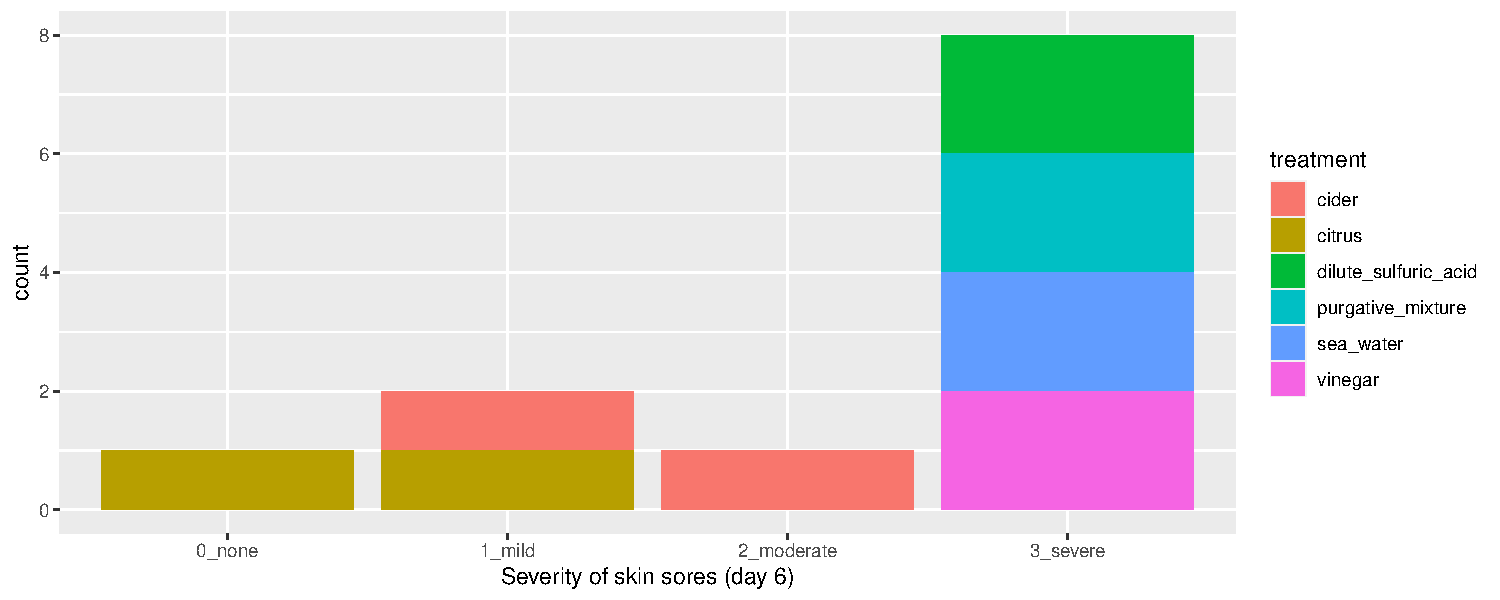
\includegraphics{CT4H_notes_files/figure-latex/unnamed-chunk-3-1.pdf}
\end{example}

A key thing to notice about the Scurvy example is that Lind went to great lengths to ensure that the treatment was the only thing affecting these 12 sailors: they all started with a similar severity of symptoms, they were kept in the same place and their diet was identical apart from their treatment. This links to one of the foundational principles of clinical trials: causal inference.

\hypertarget{causal-inference-and-clinical-trials}{%
\section{Causal inference and clinical trials}\label{causal-inference-and-clinical-trials}}

You're probably familiar with the mantra that \textbf{``correlation does not imply causation''}: just because two things are correlated, it doesn't mean we can conclude that one causes the other. If you're not convinced, \href{https://www.tylervigen.com/spurious-correlations}{here} are some humorous (and slightly macabre) examples. Causal inference is concerned with the design and analysis of data for uncovering causal relationships.

This is important for us, because we really want to be able to conclude that a treatment works (or doesn't) - that it \emph{causes} recovery, or a reduction in symptoms, or helps the patient in some way.
If we were experimental scientists in some laboratory, we could conduct some controlled experiment in which everything was kept under very specific conditions, and could fairly easily make conclusions about the treatment we were testing, and how it behaved in a range of conditions. However, testing treatments on real people is different: we don't have several identical versions of the same person to test the treatment on, and even if we did, as Gwyneth Paltrow shows us it doesn't take very much to completely alter the conditions of someone's existence!


\includegraphics{images/sliding_doors.jpeg}

Neither can we just base our conclusion of whether a treatment works on lab-based tests or theory (although undoubtedly these will both play a part in developing the treatment in the first place). The treatment needs to be tested on actual people.

Because, as we noted, people are all different, and living different lives (and unlike James Lind we can't force them all to live in the same part of a ship and eat the same food!) we will need to test the treatment on lots of people in order to gather empirical evidence. This is why statistics is so important in the design and analysis of clinical trials. The results of the trial must concluded beyond reasonable doubt, and must be able to be generalized to as-yet-untreated patients. We want to avoid any spurious correlations that are down to chance, or to associations we haven't taken into account. For example, what if the two seamen given citrus were also much younger and generally healthier than the other ten? Maybe they would have recovered quickly anyway? Or what if another treatment was actually much better than citrus, but just happened to have been given to two sailors who had some other pre-existing illness, causing them to suffer much worse with scurvy?

Clinical trials are therefore crucial for modern medicine, and statistics is crucial to clinical trials. But why exactly are clinical trials given this position of importance? Do we really have to do things this way?

\hypertarget{the-structure-of-a-clinical-trial}{%
\section{The structure of a clinical trial}\label{the-structure-of-a-clinical-trial}}

In a clinical trial, people are grouped and subdivided in various ways.

\hypertarget{the-population-of-eligible-patients}{%
\subsection*{The population of eligible patients}\label{the-population-of-eligible-patients}}
\addcontentsline{toc}{subsection}{The population of eligible patients}

One of the first steps in conducting a trial is to specify exactly what sort of person you want to test the treatment on, and where these people will be found. They may be of a certain sex and/or age range, they may have (or definitely not have) certain conditions. They may suffer from some particular symptom, or be at a particular stage of an illness.

A clear set of criteria is key to consistency. Patients are usually recruited as they present (eg. to hospital or a GP centre) and may be being recruited over several years, or by several different clinicians, so it is important that everyone is sticking to the same plan.

\begin{example}
In a study by \citet{hjalmas1998enuresis} of the use of desmopressin in children with nocturnal enuresis (bed-wetting), children had to be aged 6 - 12 with a history of PMNE (primary monosymptomatic nocturnal enuresis) and no organic pathology (no disease that alters the structure or function of organs). The children had to be free of other urinary problems (such as frequency, urgency or daytime incontinence) and not to have received any treatment for nocturnal enuresis during the 2 months before entering the trial. Children with clinically significant endocrine,
metabolic, hepatic, psychiatric, neurological, musculoskeletal, cardiovascular, haematological, renal or genitourinary disease were excluded from the trial.
\end{example}

Knowing exactly what type of patients were recruited into the trial is also key when generalizing the results to the population. If the trial recruited males aged 55-70, we cannot confidently conclude that the results will apply to a female aged 26.

\hypertarget{entry-to-the-trial}{%
\subsection*{Entry to the trial}\label{entry-to-the-trial}}
\addcontentsline{toc}{subsection}{Entry to the trial}

The group of patients recruited will be some subset of the possible population. Patients are allowed to refuse consent to take part, or individual patients may be judged unsuitable despite meeting the criteria. Knowing how many patients to recruit is a statistical question, which we will deal with soon.

\hypertarget{allocation-to-groups}{%
\subsection*{Allocation to groups}\label{allocation-to-groups}}
\addcontentsline{toc}{subsection}{Allocation to groups}

These patients are then allocated to receive either the treatment, or to be part of the control group (or more, if there are more than two groups). These groups are often referred to as the \textbf{trial arms} - the treatment arm and the control arm. Deciding which patients should be allocated to which group is another statistical question. Once the patients have been allocated, they will receive the treatment (or not) and important measurements will be taken during the trial period.

\hypertarget{comparing-results}{%
\subsection*{Comparing results}\label{comparing-results}}
\addcontentsline{toc}{subsection}{Comparing results}

Now that the trial has been run, we have two sets of measurements: one for the treatment group and one for the control group. But guess what?! Comparing these and coming to a conclusion about the effect of the treatment is a statistical question.

\hypertarget{why-bother-with-a-control-group}{%
\subsection*{Why bother with a control group?}\label{why-bother-with-a-control-group}}
\addcontentsline{toc}{subsection}{Why bother with a control group?}

Surely if we want to see whether a treatment works, we should just give it to a patient and see if they get better? Why do we need to also have a group of people not receiving the treatment?

In rare and extreme cases, this is a decent strategy: if a disease has always been fatal, but we start giving patients the treatment and some live, that is pretty solid evidence that the treatment works. This was the case with tuberculous meningitis, until the introduction of Streptomycin in 1944.

This was also the case when Edward Jenner tested cowpox as a vaccination for the fatal disease smallpox. After observing that milkmaids, once they had suffered from the mild condition cowpox (which they did often), seemed to be immune to smallpox, Jenner tested his theory by injecting an 8 year old boy called James Phipps with fluid from a milkmaid's cowpox lesions (yum). Once the boy's cowpox infection had run its course, he injected him again, this time with matter from a fresh smallpox lesion. Thankfully, James Phipps did not contract smallpox. After several more successful such tests, and a gradual shift in attitudes to the idea of vaccination (a word coined by Jenner, from the latin `vaccinia', meaning cowpox) Jenner's results were published and vaccination became commonplace. Clearly, injecting people with smallpox who had not been given the cowpox innoculation would be very cruel (they would almost certainly die) and would prove nothing; there was already plenty of evidence for the fatality of smallpox.

However, most diseases have a fairly uncertain and variable trajectory. If we give a group of patients the treatment, we can't know what would have happened to them if they hadn't received the treatment, or had received a different treatment. Comparing them to patients the past is dodgy because lots of other things may have changed since even the recent past. This is why we have a \emph{concurrent control group} (usually known as just the \emph{control group}). These patients do not receive the new treatment, but instead carry on as usual. The aim is to make the control and treatment groups as similar as possible in all other respects (especially those we deem important) so that at the end we can attribute the difference between the two groups to the treatment.

\hypertarget{primout}{%
\section{The primary outcome}\label{primout}}

In a clinical trial, there are usually many measurements performed on patients, and possibly at various different points throughout the trial. However, for the sake of the analysis, we usually determine one to be the \textbf{primary outcome variable}. The research questions should be phrased in terms of this variable, and the goal of our design should be to be able to answer questions about this variable.

\begin{example}
In a trial by \citet{villar2020dexamethasone} investigating the use of Dexamethasone treatment for acute respiratory distress syndrome , the primary outcome was the `number of ventilator free days up to 28 days', while other outcomes included `all-cause mortality after 60 days' and `incidence of infections in ICU'.
\end{example}

\hypertarget{ethical-issues}{%
\section{Ethical issues}\label{ethical-issues}}

Clinical trials differ from most scientific experiments in that they are experimenting on people. This means that the team designing, conducting and analysing the trial have various ethical responsibilities. This is a huge area; we will touch on it from time to time but will not go into anywhere near enough detail! Some key things to note though are\ldots.

\begin{itemize}
\tightlist
\item
  A patient must never be given a treatment that is known to be inferior.
\item
  Patients must be fully informed about the trial, the treatments used, possible adverse effects and side-effects and so on. Patients should only be recruited into the trial if, after being given all this information (and having had it communicated clearly and at an appropriate level) they give their consent.
\item
  After entering a trial, a patient has the right to withdraw at any point, and should then receive whatever treatment is most appropriate for them. They should not face any negative repurcussions for withdrawing.
\end{itemize}

The patients' interests are safeguarded by the \href{https://www.wma.net/policies-post/wma-declaration-of-helsinki-ethical-principles-for-medical-research-involving-human-subjects/}{Declaration of Helsinki}. This statement is implemented differently by different countries. In the UK, health authorities each have their own ethics committee, by which proposals for experiments involving human subjects must be approved.

You might think that these ethical issues largely concern the clinicians, and that we statisticians don't need to worry too much about the ethics of clinical trials. After all, we are likely never to meet any patients or to get our hands dirty in any way! But as we will see, at each stage the choices made by the statistician can in fact have serious ethical implications.

\hypertarget{phases-of-clinical-trials}{%
\section{Phases of clinical trials}\label{phases-of-clinical-trials}}

If you read about clinical trials (or hear about them in the news), you'll hear talk of a `phase 3 trial' or similar. Broadly speaking, clinical trials follow a progression from phase one (or sometimes zero) to phase four. These phases apply to most countries, and any for any drug to be licensed multinationally it must get through phase III.

\hypertarget{phase-zero}{%
\subsection*{Phase zero}\label{phase-zero}}
\addcontentsline{toc}{subsection}{Phase zero}

The first step is to test a low dose of the treatment on a small number of people, to check that it isn't harmful. The dose is too low to have any medicinal effect, but is designed to verify that the drug behaves as expected from laboratory studies, and doesn't have any harmful effects. There may only be 10-20 participants, and there is no randomisation (or control group).

\hypertarget{phase-one}{%
\subsection*{Phase one}\label{phase-one}}
\addcontentsline{toc}{subsection}{Phase one}

Phase one trials are also quite small (around 20-50 participants) and are designed to find the best dose of the treatment and what any side effects are. Phase one trials tend to be recruited very slowly: a small group will be recruited onto a low dose and monitored closely. If all goes well, another small group will be recruited on a slightly higher dose, and so on. This is known as a \emph{dose escalation study}. Participants at this phase are monitored very closely, for example through regular blood tests and recording daily symptoms.

\hypertarget{phase-two}{%
\subsection*{Phase two}\label{phase-two}}
\addcontentsline{toc}{subsection}{Phase two}

If the drug makes it through the phase one trial, it can progress to phase two (often written as `phase II'). These involve more people than phase one, possibly up to 100. The cohort may now be restricted to people with a particular version of a condition (eg. a particular type of cancer), but it may still be broader than the sorts of trials we will be looking at. Now the aim is to find out if the new treatment works well enough to progress to a large phase three (phase III) trial:

\begin{itemize}
\tightlist
\item
  Exactly what conditions (or versions of a condition) does this treatment work for?
\item
  What are the side effects and can they be managed?
\item
  What is the best dose to administer?
\end{itemize}

Phase II trials sometimes compare the treatment to a placebo, and sometimes use randomisation to group participants.

This is the stage at which most drugs fail, for a multitude of reasons (cost, safety, efficacy,\ldots).

\hypertarget{phase-three}{%
\subsection*{Phase three}\label{phase-three}}
\addcontentsline{toc}{subsection}{Phase three}

Phase III trials are much bigger, often involving hundreds or thousands of participants, and aim to compare the new treatment to the best currently available treatment (which may be another treatment, or may be nothing). Side effects are still monitored, as some of the rarer ones may not show themselves at the smaller phases, because there are fewer participants.

In phase III trials, the aim is to find out if the new treatment is better, and if so by how much. Phase III trials almost always use randomisation to allocate participants to groups, and go to great lengths to make the trial as reliable as possible, for example using a placebo for the control group (who aren't getting the real treatment) that looks identical to the real drug. These are the sorts of trials we will mainly be concerned with in this course.

To be licensed, a treatment has to get through phase III and be found to be effective (and of course safe).

\hypertarget{phase-four}{%
\subsection*{Phase four}\label{phase-four}}
\addcontentsline{toc}{subsection}{Phase four}

Phase IV trials happen after the treatment has been found to work, has been licensed and is in use. The aims of phase IV trials are

\begin{itemize}
\tightlist
\item
  to find out more about the rarer side effects
\item
  to investigate the long term risks and benefits
\item
  to find out how well the treatment works when given to a broader group of people than in phase III.
\end{itemize}

\hypertarget{part-part-i-continuous-outcome-variables}{%
\part{Part I: Continuous outcome variables}\label{part-part-i-continuous-outcome-variables}}

\hypertarget{rct-plan}{%
\chapter{Sample size for a normally distributed primary outcome variable}\label{rct-plan}}

For most of this module, we'll focus on randomised controlled trials (RCTs). These have mainly been used for clinical applications (for example, to test a particular drug), but have also recently become popular ways to test interventions in areas such as education and policing.

Having laid the groundwork in Chapter \ref{rct-intro}, we now go on to some more technical details. In this Chapter, we focus on the `vanilla' scenario, where we have a trial with two arms, and our unit of randomization is individuals. At first we will focus only on continuous outcomes, but in later weeks we will go on to think about binary and time-to-event data.

Broadly speaking, the topics we cover fall into the categories of `before the trial' (design and planning) or `after the trial' (analysis), although as we'll see there is some interaction between these stages.

The first big question asked of a trial statistician is usually how many participants does the trial need in order to be viable: the sample size. We will clarify what is meant by `viable' later in this section.

Broadly speaking, there are two (opposing) ethical issues around sample size:

\begin{enumerate}
\def\labelenumi{\arabic{enumi}.}
\tightlist
\item
  If we don't recruit enough patients, then we may not gather enough evidence to draw any conclusion about the research question (eg. whether there is a treatment effect). As well as being scientifically disappointing, this is unethical. To conduct the trial, some of the patients will have been subject to an inferior treatment (assuming one treatment was actually better), and if there is no conclusion then this was effectively for no purpose.
\item
  If we recruit too many patients (ie. we would be sufficiently likely to reach a conclusion with many fewer) then we have subjected more patients than necessary to an inferior treatment, and possibly also taken up more time and resources than was necessary.
\end{enumerate}

Therefore it is important to think about this issue carefully. We've framed the question in quite a woolly way so far, but now we'll start to think more carefully.

\hypertarget{the-treatment-effect}{%
\section{The treatment effect}\label{the-treatment-effect}}

In Section \ref{primout} we discussed the need to settle on a \textbf{primary outcome variable}. One reason this is important is that we base our sample size calculations on the primary outcome variable.

\begin{definition}
Suppose our primary outcome variable is \(X\), which has mean \(\mu\) in the control group and mean \(\mu + \tau\) in the treatment group. The variable \(\tau\) is the \textbf{treatment effect}. The goal of our RCT is to learn about \(\tau\). The larger \(\tau\) is (in magnitude), the more pronounced the effect of the intervention.
\end{definition}

This problem is usually framed as a \textbf{hypothesis test}, where the null hypothesis is that \(\tau=0\).

\hypertarget{reminder-hypothesis-tests-with-a-focus-on-rcts}{%
\section{Reminder: hypothesis tests (with a focus on RCTs)}\label{reminder-hypothesis-tests-with-a-focus-on-rcts}}

When performing a hypothesis test, what we are aiming to find is the \textbf{P-value}.

\begin{definition}
The \textbf{P-value} is the probability of obtaining a result as extreme or more extreme (ie. further away from the null hypothesis value) than the one obtained \emph{given that the null hypothesis is true}.
\end{definition}

Put simply, the p-value is a measure of the probability of obtaining whatever result (eg. treatment effect) we have have found simply by random chance, when in fact there is no treatment effect (ie. \(\tau=0\)). Generally, a P-value of \(\alpha = 0.05\) is accepted as sufficient evidence to reject the null hypothesis, although in clinical settings it can often be smaller (eg. \(\alpha = 0.01\)). It is conventional to present the P-value by simply saying whether it is smaller than some threshold (often 0.05), rather than giving the exact value.

\begin{definition}
The threshold for the p-value below which the results are considered `significant' is known as the \textbf{significance level} of the test, and is generally written \(\alpha\) (as above).
\end{definition}

This use of a significance level is (in part) a legacy from early days when computers were rare and values were looked up in \(t\)-tables (or similar). Now that it is very simple to find the exact P-value, it is becoming more and more common to report the actual number. Indeed, there is a big difference between \(p=0.049\) and \(p=0.000049\).

\hypertarget{insignificant-results}{%
\subsection{Insignificant results}\label{insignificant-results}}

If our P-value is relatively large, say 0.3 or 0.5 (or really, greater than \(\alpha\)), then our result is not at all unlikely (or sufficiently unlikely) under the null hypothesis, and provides insufficient evidence to reject \(H_0\). However, it is not inconsistent with the existence of a treatment effect, so we don't say there is evidence to accept \(H_0\). One can imagine that if the true treatment effect \(\tau\) were tiny, many trials would fail to find evidence to reject \(H_0\). However, if our sample size were sufficiently large, we should be able to detect it. Conversely, if \(\tau\) is very large, even a relatively small sample size is likely to provide enough evidence to reject \(H_0\).

A non-significant P-value means that our results are consistent with the null hypothesis \(\tau=0\), but they are also consistent with some small treatment effect, and therefore we can't conclude very much. The key issue is, what size of treatment effect do we care about? We must ensure that our sample size is sufficiently large to be sufficiently likely to detect a clinically meaningful treatment effect.

We are being vague for now, but this is a key issue in determining an appropriate sample size.

\hypertarget{one-tailed-or-two-tailed}{%
\subsection{One-tailed or two-tailed?}\label{one-tailed-or-two-tailed}}

It is highly likely that the scientists running the trial will have a strong idea of the likely `direction' of the treatment effect. Assuming that a larger value of the primary outcome variable \(X\) is good, they will expect a positive value of the treatment effect \(\tau\) (or be prepared to accept a possible value of zero for no effect).

It would therefore be tempting to perform a one-sided test, with

\begin{align*}
  H_0\,&:\, \tau=0\\
  H_1\,&:\, \tau>0.
\end{align*}

For example, suppose our test statistic \(t\) has a \(t\) distribution with 31 degrees of freedom and we obtain a value of 2, as shown in Figure \ref{fig:t31-onesided}.
In this case our P-value is \(1 - F_t\left(2, df=31\right)= 0.0272\) (where \(F_t\left(\cdot\right)\) is the cumulative distribution function of the \(t\) distribution) , and the result would be considered significant at the 0.05 level.

\begin{figure}
\centering
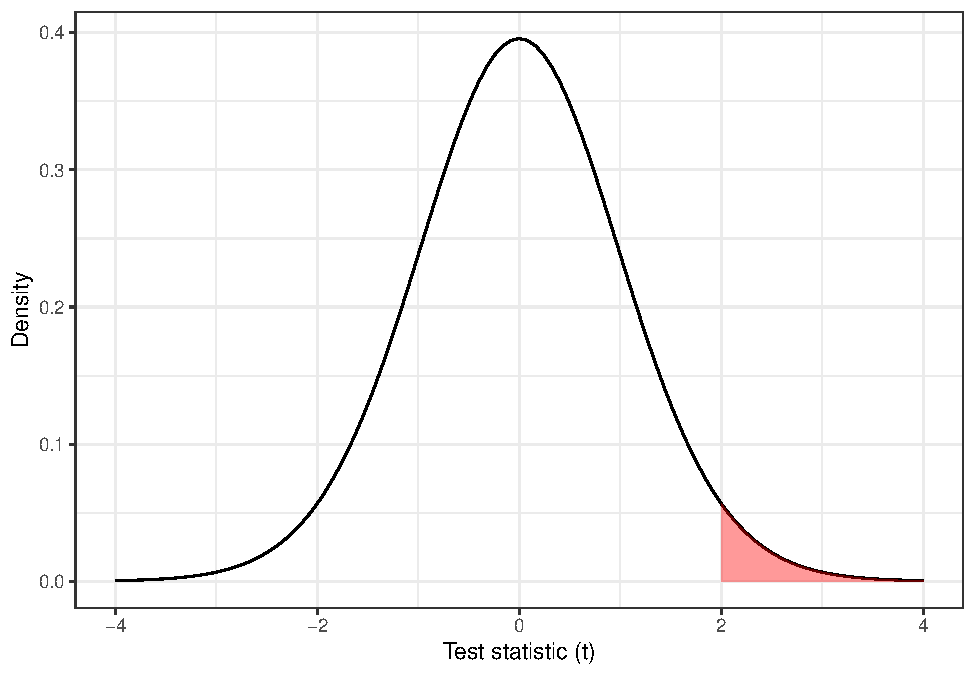
\includegraphics{CT4H_notes_files/figure-latex/t31-onesided-1.pdf}
\caption{\label{fig:t31-onesided}The distribution \(t_{31}\), with the area corresponding to \(t > 2\) shaded.}
\end{figure}

For a large positive value of \(t\), we obtain a small P-value, and reject \(H_0\), concluding that the intervention is effective (in a good way). However, what if we obtain a large negative value of \(t\)? In this one-sided set-up, there is no value of \(t<0\) that would give a significant result; negative values of \(t\) are simply considered consistent with \(H_0\), and there is no mechanism to conclude that an intervention has a significantly negative effect.

For this reason, we always conduct two sided hypothesis tests, with

\begin{align*}
  H_0\,&:\, \tau=0\\
  H_1\,&:\, \tau\neq 0.
\end{align*}

In this scenario, Figure \ref{fig:t31-onesided} is replaced by the plot shown in Figure \ref{fig:t31-twosided}, where values of \(t\) with \(t<-2\) are considered `equivalent' to those with \(t>2\), in the sense of how unlikely they are under \(H_0\).

\begin{figure}
\centering
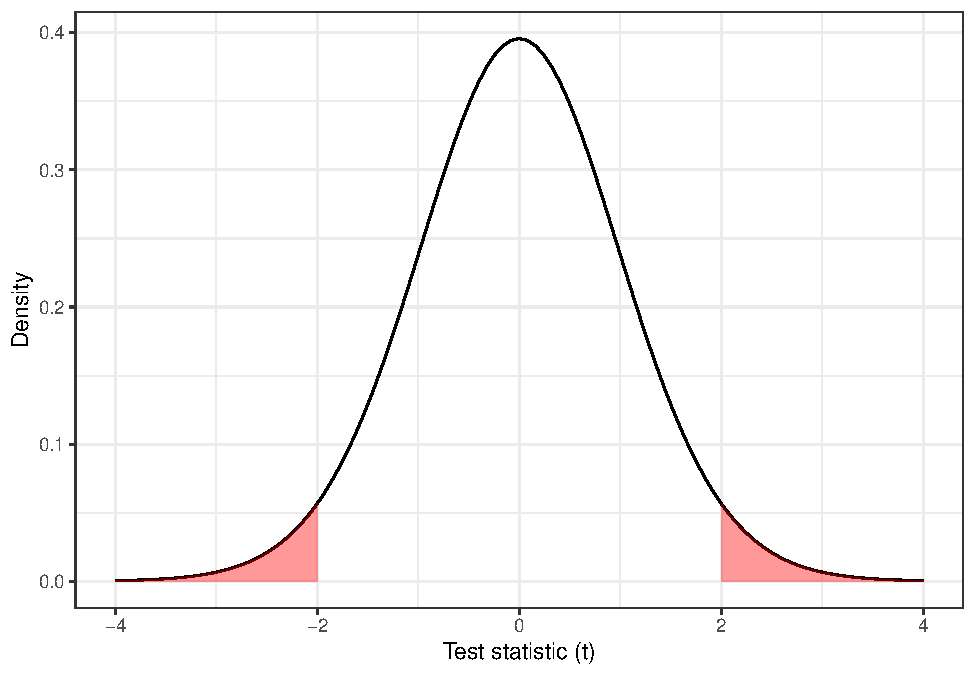
\includegraphics{CT4H_notes_files/figure-latex/t31-twosided-1.pdf}
\caption{\label{fig:t31-twosided}The distribution \(t_{31}\), with the area corresponding to \(|t| > 2\) shaded.}
\end{figure}

The P-value for the two-sided test as shown in Figure \ref{fig:t31-twosided} is

\[ F\left(-2, df=31\right) + \left[1 - F\left(2, df=31\right)\right] = 2\times{0.0272} = 0.0543\]
and the result is no longer significant at the 0.05 level. Throughout this course, we will always assume two-tailed tests.

\begin{figure}
\centering

\includegraphics{images/starbucks.jpg}
\caption{\label{fig:starbucks}A rather ubiquitous two-tailed mermaid}
\end{figure}

\hypertarget{sec-measDcont}{%
\section{Constructing a measure of effect size}\label{sec-measDcont}}

Let's say we are recruiting participants into two groups: group \(T\) will be given the new treatment (they will sometimes be referred to as the \emph{treatment group} or \emph{treatment arm}) and group \(C\) will be given the control (they are the \emph{control group} or \emph{control arm}).

Suppose that we have \(n\) patients in group \(C\), and \(m\) in group \(T\). The primary outcome variable \(X\) is normally distributed with mean \(\mu\) in group C (the control group) and mean \(\mu+\tau\) in group T (the intervention group), and common standard deviation \(\sigma\). So

\begin{align*}
X & \sim N\left(\mu, \sigma^2\right) \text{ in group }C\\
X & \sim N\left(\mu + \tau, \sigma^2\right) \text{ in group }T.
\end{align*}

We are testing the null hypothesis \(H_0: \tau=0\) against the alternative hypothesis \(H_1: \tau\neq{0}\).

Using the data obtained in the trial, we will be able to obtain sample means \(\bar{x}_C\) and \(\bar{x}_T\) from each group, and a pooled estimate of the standard deviation

\[ s = \sqrt{\frac{\left(n-1\right)s_C^2 + (m-1)s_T^2}{n+m - 2}},
\]
where \(s_C\) and \(s_T\) are the sample standard deviations for groups \(C\) and \(T\) respectively, for example

\[
s_C = \sqrt{\frac{\sum\limits_{i=1}^n{\left(x_i - \bar{x}_C\right)^2}}{n-1}}.
\]

Using these values we can compute

\[D = \frac{\bar{x}_T - \bar{x}_C}{s\sqrt{\frac{1}{n} + \frac{1}{m}}}\]
as a standardised measure of the effect \(\tau\).

\begin{theorem}
Under \(H_0\), \(D\) has a \(t\)-distribution with \(n+m-2\) degrees of freedom.
\end{theorem}

\begin{proof}
Under \(H_0\) the \(x_i\) are iid \(N\left(\mu,\;\sigma^2\right)\), and so

\begin{align*}
\bar{x}_C & \sim{N\left(\mu, \frac{\sigma^2}{n}\right)}\\
\bar{x}_T & \sim{N\left(\mu, \frac{\sigma^2}{m}\right)}
\end{align*}

and therefore

\[
\bar{x}_T - \bar{x}_C \sim{N \left(0, \sigma^2\left[\frac{1}{n} + \frac{1}{m}\right] \right)}\]

and
\[
\frac{\bar{x}_T - \bar{x}_C}{\sigma \sqrt{\frac{1}{n}+\frac{1}{m}}} \sim{N\left(0,1\right)}.\]

We know that for \(x_1,\ldots,x_n,\sim N\left(\mu,\sigma^2\right)\) for some arbitrary \(\mu\) and \(\sigma^2\),

\[\frac{1}{\sigma^2}\sum\limits_{i=1}^n\left(x_i - \bar{x}\right)^2 \sim{\chi^2_{n-1}},\]
and so we have

\begin{align*}
\frac{n-1}{\sigma^2}s_C^2 & \sim \chi^2_{n-1}\\
\frac{m-1}{\sigma^2}s_T^2 & \sim \chi^2_{m-1}\\
\text{and} &\\
\frac{1}{\sigma^2}\left[\left(n-1\right)s_C^2 + \left(m-1\right)s_T^2\right] & = \frac{n+m-2}{\sigma^2}s^2\\
&\sim \chi^2_{n+m-2}.
\end{align*}

The definition of a \(t\)-distribution is that if \(Z\sim N\left(0,1\right)\) and \(Y \sim{\chi^2_n}\) then

\[X = \frac{Z} {\sqrt{\frac{Y}{n}}} \sim{t_n},\]
that is \(X\) has a \(t\) distribution with \(n\) degrees of freedom.

Plugging in our \(N\left(0,1\right)\) variable for \(Z\) and our \(\chi^2_{n+m-2}\) variable for \(Y\), we have

\begin{align*}
\frac{\frac{\bar{x}_T - \bar{x}_C}{\sigma\sqrt{\frac{1}{n} + \frac{1}{m}}}}{\sqrt{\left(\frac{n+m-2}{\sigma^2}s^2\right) \bigg/ \left(n+m-2\right)}} & = \frac{\bar{x}_T - \bar{x}_C}{\sigma\sqrt{\frac{1}{n} + \frac{1}{m}}} \bigg/ \frac{s}{\sigma} \\
& = \frac{\bar{x}_T - \bar{x}_C}{s\sqrt{\frac{1}{n} + \frac{1}{m}}} \\
& = D
\end{align*}

and therefore \(D\) has a \(t\) distribution with \(n+m-2\) degrees of freedom.
\end{proof}

We can therefore use \(D\) as our test statistic; if \(D\) is such that

\[ |D| > t_{n+m-2}\left(\alpha/2\right)\]
where
\(t_{n+m-2}\left(\cdot\right)\) is the function such that \(P\left(T>t_{df}\left(\xi\right)\right) = \xi\) when \(T \sim{t_{df}}\) then we can reject \(H_0\).

In practical terms, for more than around 40 degrees of freedom, the \(t\) distribution is indistinguishable from the normal distribution, and since it is rare to have fewer than 40 participants in an RCT, we use a normal approximation in what follows, and a difference is significant at the \(100\left(1-\alpha\right) \%\) level if \(|D| > z_{\alpha/2}\), where \(z\) are standard normal quantile values. For example, for \(\alpha=0.05\) have \(z_{\alpha/2} = 1.960\), since the probability of a standard normal variable exceeding this value is 0.025.

So, if we have run a trial, and have obtained \(n\) values of \(X\) from group \(C\) and \(m\) values of \(X\) from group \(T\), we can compute \(D\). If \(D\) lies outside the interval \(\left[-z_{\alpha/2}, z_{\alpha/2}\right]\) then we reject \(H_0\).

This is equivalent to \(\bar{x}_T - \bar{x}_C\) falling outside the interval

\[\left[-z_{\alpha/2}s\sqrt{\frac{1}{n} + \frac{1}{m}},\; z_{\alpha/2}s\sqrt{\frac{1}{n} + \frac{1}{m}}  \right]. \]

\hypertarget{brief-aside-on-notation}{%
\subsubsection*{Brief aside on notation}\label{brief-aside-on-notation}}
\addcontentsline{toc}{subsubsection}{Brief aside on notation}

\emph{We'll see a lot of the notation \(z_{\alpha/2}\) and similar, so to clarify:}

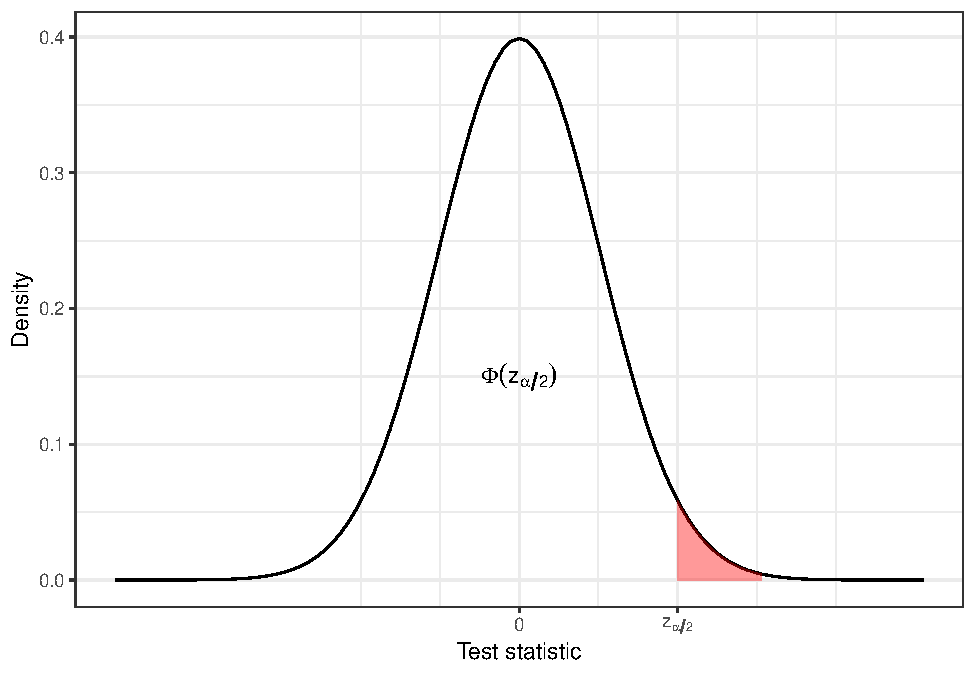
\includegraphics{CT4H_notes_files/figure-latex/unnamed-chunk-5-1.pdf}

\emph{In R, we have \(\Phi\left(z_{\alpha/2}\right) = \texttt{pnorm}\left(z_{\alpha/2}\right)\) and \(z_{\alpha/2} = \texttt{qnorm}\left(\Phi\left(z_{\alpha/2}\right)\right)\). \texttt{qnorm} is the quantile and \texttt{pnorm} is the cumulative distribution function. So, for example}
\[\frac{\alpha}{2} = 1 - \Phi\left(z_{\alpha/2}\right)\]

We have constructed our whole argument under the assumption that \(H_0\) is true, and that the probability of such a value is therefore \(\alpha\). We want this probability to be small, since it constitutes an error; \(H_0\) is true, but our value of \(D\) (or the difference in means) leads us to reject \(H_0\). This is sometimes called the `type I' error rate. But what if \(H_0\) is false?

\hypertarget{sec-power}{%
\section{\texorpdfstring{Power: If \(H_0\) is false}{Power: If H\_0 is false}}\label{sec-power}}

We have constructed things so that if \(H_0\) is true, we have a small probability of rejecting \(H_0\). But if \(H_0\) is false, and \(\tau\neq{0}\), we want our test to have a high probability of rejecting \(H_0\).

\begin{definition}
The \textbf{power} of a test is the probability that we reject \(H_0\), given that \(H_0\) is false. The \textbf{power function} depends on the value of \(\tau\) and is

\[\Psi\left(\tau\right) = \Pr\left(\text{Reject } H_0\mid{\tau\neq{0}}\right) = 1 - \beta.\]
The quantity \(\beta\) therefore represents \(\Pr\left(\text{Fail to reject } H_0\mid{\tau\neq{0}}\right)\), which is the \textbf{type II error rate}.
\end{definition}

If you find the notation confusing (as I do!) then it might be helpful to remember that both \(\alpha\) and \(\beta\) are \textbf{error rates} - probabilities of coming to the wrong conclusion. It is common to talk in terms of \(\alpha\), the significance level, (which will be a low number, often 0.05) and of \(1-\beta\), the power (which will be a high number, often 0.8). I've found though that it is not uncommon to find people refer to \(\beta\) (rather than \(1-\beta\)) as the power. If in doubt, keep in mind that we require \(\alpha,\;\beta \ll 0.5\). It is also common to use percentages: a significance level of \(\alpha=0.05\) can also be referred to as ``the 95\% level'', and \(\beta=0.2\) is the same as a ``power of 80\%''. When using percentages, we talk in terms of the amount of time we expect the test to come to the correct conclusion.

If you notice any mistakes in these notes along these (or other!) lines, please point them out.

Under \(H_1\), we have (approximately)

\[D \sim{N\left(\frac{\tau}{\sigma\lambda\left(n,m\right)}, 1\right)},\]
where \(\lambda\left(n,m\right) = \sqrt{\frac{1}{n}+\frac{1}{m}}\) and
\[D = \frac{\bar{x}_T - \bar{x}_C}{s\sqrt{\frac{1}{n} + \frac{1}{m}}}.\]

Figure \ref{fig:accepth0} shows the distribution of \(D\) under \(H_0\) and \(H_1\) for some arbitrary (non-zero) effect size \(\tau\). The turquoise bar shows the acceptance region of \(H_0\), ie. the range of observed values of \(D\) for which we will fail to reject \(H_0\). We see that this contains 95\% of the area of the \(H_0\) distribution (we have set \(\alpha = 0.05\) here), so under \(H_0\), we have a 0.95 probability of observing a value of \(D\) that is consistent with \(H_0\).

\begin{figure}
\centering
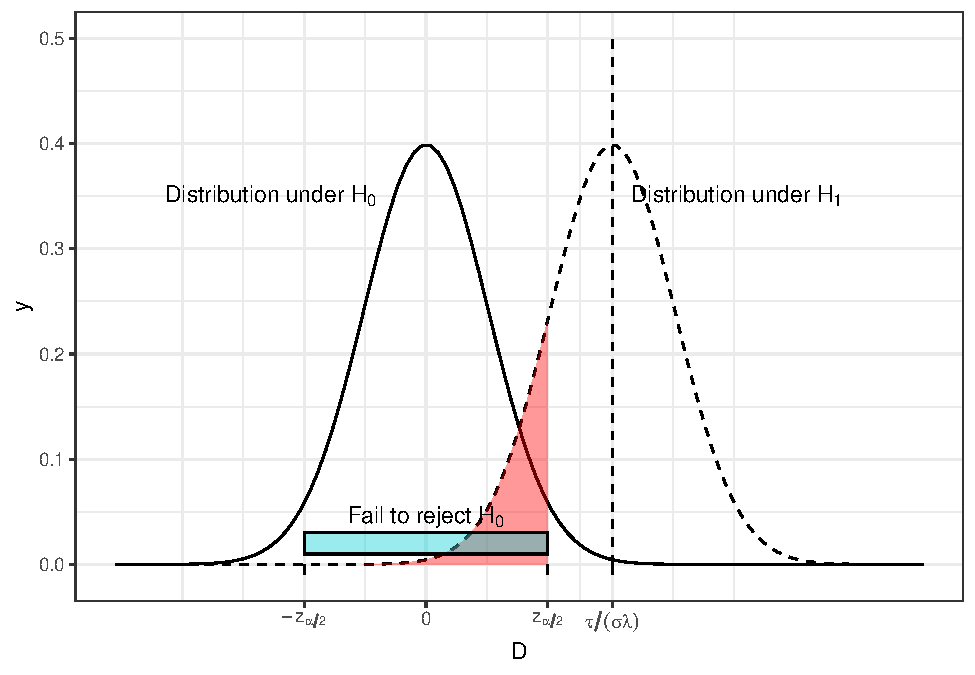
\includegraphics{CT4H_notes_files/figure-latex/accepth0-1.pdf}
\caption{\label{fig:accepth0}The distribution of \(D\) under both \(H_0\) and \(H_1\) for some arbitrary values of effect size, population variance, \(n\) and \(m\), with the region in which we fail to reject \(H_0\) shown by the turquoise bar and the red shading.}
\end{figure}

However, if \(H_1\) is true, and \(\tau\neq{0}\), there is a non-zero probability of observing a value of \(D\) that would lead us to fail to reject \(H_0\). This is shown by the area shaded in red, and it has area \(\beta\). One minus this area (ie. the area under \(H_1\) that leads us to accept \(H_1\)) is the power, \(1-\beta\).

We can see that if the distributions have better separation, as in Figure \ref{fig:accepth0-1}, the power becomes greater. This can be as a result of a larger \(\tau\), a smaller \(\sigma\) or a smaller \(\lambda\) (therefore larger \(m\) and/or \(n\)).

\begin{figure}
\centering
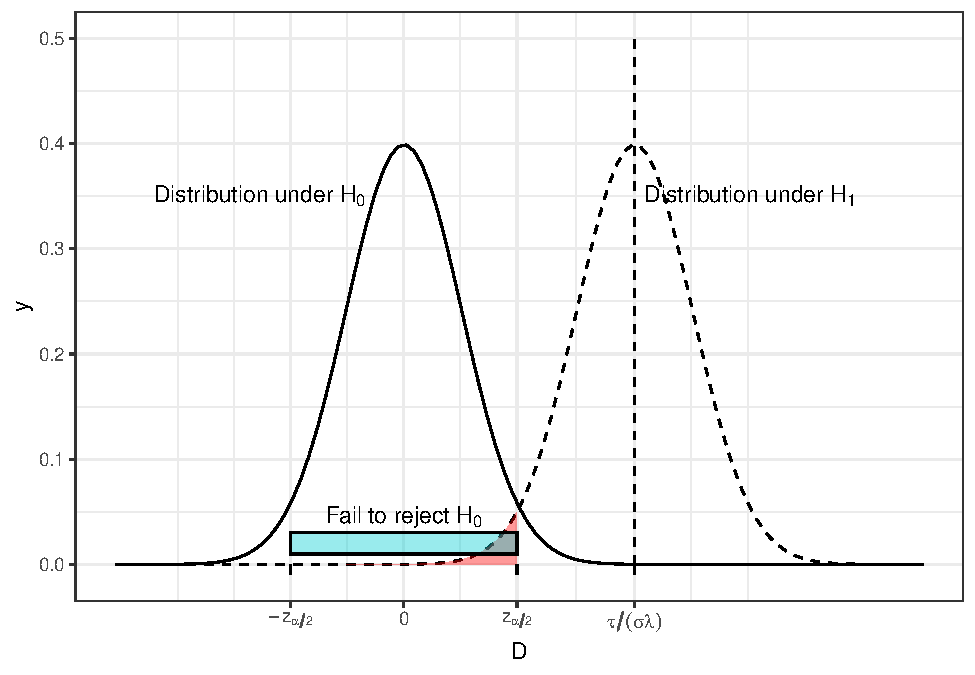
\includegraphics{CT4H_notes_files/figure-latex/accepth0-1-1.pdf}
\caption{\label{fig:accepth0-1}The distribution of D under both \(H_0\) and \(H_1\) for some arbitrary values of effect size, population variance, \(n\) and \(m\), with the region in which we fail to reject \(H_0\) shown by the turquoise bar and the red shading.}
\end{figure}

For given values of \(\alpha\), \(\sigma\) and \(\lambda\left(n,m\right)\), we can calculate the power function in terms of \(\tau\) by finding the area of the distribution of \(D\) under \(H_1\) for which we accept \(H_1\).

\begin{equation}
\Psi\left(\tau\right) = 1-\beta = \left[1 - \operatorname{\Phi}\left(z_{\frac{\alpha}{2}} - \frac{\tau}{\sigma\lambda}\right)\right] + \operatorname{\Phi}\left(-z_{\frac{\alpha}{2}} - \frac{\tau}{\sigma\lambda}\right)
\label{eq:powerfun}
\end{equation}

The first term in Equation \eqref{eq:powerfun} is the area in the direction of \(\tau\). In Figures \ref{fig:accepth0} and \ref{fig:accepth0-1} this is the region to the right of the interval for which we fail to reject \(H_0\), ie. where \[D > z_{\frac{\alpha}{2}}.\]

The second term in Equation \eqref{eq:powerfun} represents the area away from the direction of \(\tau\), ie. a value of \(D\) such that

\[ D < - z_{\frac{\alpha}{2}},\]
assuming without loss of generality that \(\tau>0\).

Figure \ref{fig:powercurve} shows the power function \(\Psi\left(\tau\right)\) for \(\tau\) in units of \(\sigma\) (or you could think of this as for \(\sigma=1\)), for three different pairs of values of \(n\) and \(m\) (remember that these enter the power function via \(\lambda\)) with \(\alpha=0.05\). We see that in general the power is higher for larger sample sizes, and that of the two designs where \(n+m=200\), the balanced one with \(n=m=100\) achieves the greatest power.

In general, the probability of rejecting \(H_0\) increases as \(\tau\) moves away from zero.

Notice also that all the curves pass through the point \(\tau=0,\,\beta=0.05\). Since \(\tau=0\) corresponds to \(H_0\) being true, it makes sense that the probability of rejecting the \(H_0\) is the significance level \(\alpha\).

\begin{figure}
\centering
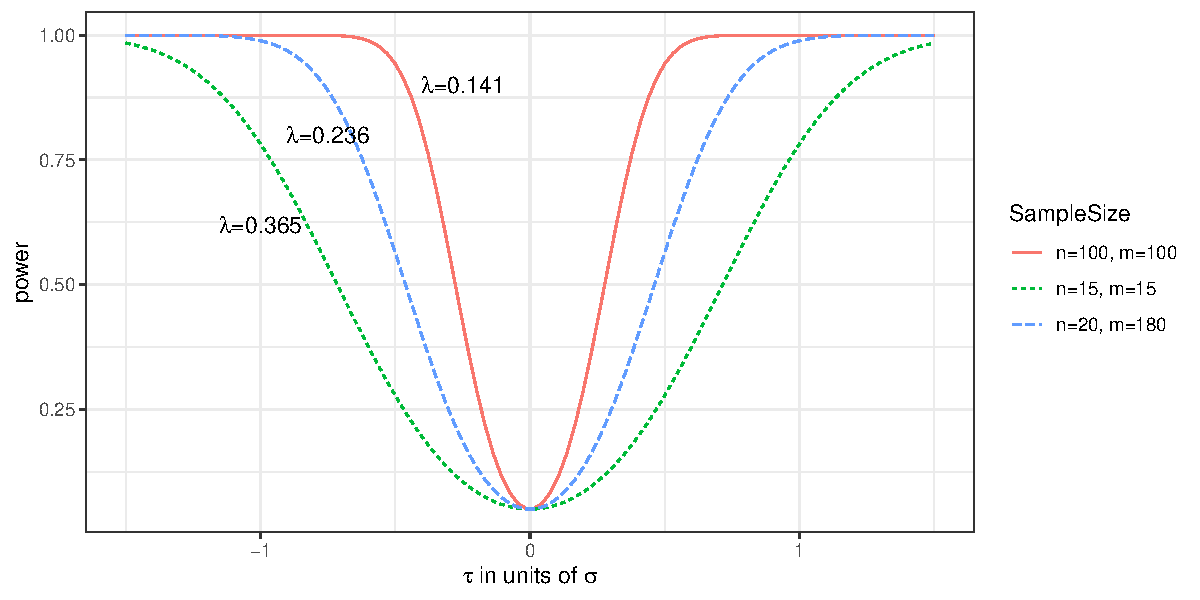
\includegraphics{CT4H_notes_files/figure-latex/powercurve-1.pdf}
\caption{\label{fig:powercurve}Power curves for various values of \(n\) and \(m\), with effect size in units of standard deviation, given a type I error rate of 0.05.}
\end{figure}

It is common to think of the effect size in units of \(\sigma\), as we have done here. This makes results more intuitive, since we don't need to have a good knowledge of the actual outcome variable to know what is a small or large effect size. It is also helpful in situations where the population standard deviation is not well understood, since the trial can be planned with this sort of effect size in mind. To denote the effect size in units of \(\sigma\), we will write \(\tau_\sigma\), although in practice it is more usual to give both the same notation.

\hypertarget{sec-ssformulacont}{%
\section{A sample size formula}\label{sec-ssformulacont}}

Equation \eqref{eq:powerfun} allows us to find any one of \(\tau_\sigma,\,\alpha,\,\beta\) and \(\lambda\left(n,m\right)\) given values for the others. Values for \(\alpha\) and \(\beta\) are often specified by those planning the trial as around \(\alpha \in \left[0.01,0.05\right],\,1-\beta\in\left[0.8,0.9\right]\).

The remaining two variables, \(\tau_\sigma\) and \(\lambda\left(n,m\right)\) are generally settled using one or both of the following questions:

\begin{itemize}
\tightlist
\item
  Given our budget constraints, and their implications for \(n\) and \(m\), what is the smallest value of \(\tau_\sigma\) we can achieve?
\item
  What is the smallest value of \(\tau_\sigma\) that would be clinically useful to detect, and what value of \(\lambda\left(n,m\right)\) do we need in order to achieve it?
\end{itemize}

In a medical setting, an estimate of \(\sigma\) is usually available, and so we will return to thinking in terms of \(\tau\) and \(\sigma\). In this equation, the value we use (or find) for \(\tau\) is the \textbf{minimum detectable effect size}, which we will denote \(\tau_M\).

\begin{definition}
The \textbf{minimum detectable effect size} \(\tau_M\) for a particular trial is the smallest value of effect size that is able to be detected with power \(1-\beta\) and at significance level \(\alpha\) (for some specified values of \(\alpha,\;\beta\)).
\end{definition}

Note that we will not \emph{definitely} detect an effect of size \(\tau_M\), if it exists; by construction, we will detect it with probability \(1-\beta\). If \(|\tau| > |\tau_M|\) (ie. the true effect size is further from zero than \(\tau_M\) is) then the probability of detecting it will be greater than \(1-\beta\). If \(|\tau| < |\tau_M|\) then the probability of detecting it will be less than \(1-\beta\).

Although we could solve Equation \eqref{eq:powerfun} numerically, in practice we use an approximation. The second term, representing observed values of \(D\) that are far enough away from 0 \emph{in the opposite direction from the true \(\tau\)} to lead us to reject \(H_0\) is so negligible as to be able to be discounted entirely. Indeed, if we were to observe such a value of \(D\), we would come to the wrong conclusion about \(\tau\).

Therefore, Equation \eqref{eq:powerfun} becomes

\begin{equation}
\Psi\left(\tau\right) = 1-\beta = \left[1 - \operatorname{\Phi}\left(z_{\frac{\alpha}{2}} - \frac{\tau_M}{\sigma\lambda}\right)\right].
\label{eq:powerfun2}
\end{equation}

Because \(\operatorname{\Phi}\left(z_\beta\right) = 1 - \beta\) (by definition) and \(\operatorname{\Phi}\left(-z\right) = 1 - \operatorname{\Phi}\left(z\right)\) we can write this as

\[ \operatorname{\Phi}\left(z_\beta\right) = \operatorname{\Phi}\left(\frac{\tau_M}{\sigma\lambda} - z_{\frac{\alpha}{2}}\right), \]
where \(\tau_M\) is our minimum detectable effect size. Because of the monotonicity of \(\operatorname{\Phi}\left(\cdot\right)\), this becomes

\begin{equation}
\begin{aligned}
  z_\beta & = \frac{\tau_M}{\sigma\lambda} - z_{\frac{\alpha}{2}} \\
  z_\beta + z_{\frac{\alpha}{2}} & = \frac{\tau_M}{\sigma\lambda}.
\end{aligned}
\label{eq:powerfun3}
\end{equation}

Because we want to think about sample sizes, we rewrite this further. It is most common to perform trials with \(n=m=N\) participants in each group, in which case

\[ \lambda\left(n,m\right) = \sqrt{\frac{2}{N}}\]

and Equation \eqref{eq:powerfun3} rearranges to

\begin{equation}
    N = \frac{2\sigma^2\left(z_\beta + z_{\frac{\alpha}{2}}\right)^2}{\tau_M^2}.
    \label{eq:sscont}
\end{equation}

\begin{example}
\citep[from][]{zhong2009calculate}
A trial is being planned to test whether there is a difference in the efficacy of ACEII antagonist (a new drug) and ACE inhibitor (the standard drug) for the treatment of primary hypertension (high blood pressure). The primary outcome variable is change in sitting diastolic blood pressure (SDBP, mmHg) compared to a baseline measurement taken at the start of the trial. The trial should have a significance level of \(\alpha=0.05\) and a power of \(1-\beta = 0.8\), with the same number of participants in each group. The minimum clinically important difference is \(\tau_M = 3 \text{ mmHg}\) and the pooled standard deviation is \(s = 8 \text{ mmHg}\). Therefore, using equation \eqref{eq:sscont} the sample size should be at least

\begin{align*}
      N & = \frac{2\times{8}^2\left(0.842 + 1.96\right)^2}{3^2}\\
      & = 111.6,
\end{align*}

and therefore we need at least 112 participants in each trial arm.
\end{example}

\hypertarget{allocation}{%
\chapter{Allocation}\label{allocation}}

Once we've decided how many participants we need in our trial, and they've been recruited, we next need to determine which participants should be assigned to which trial arm. This is process is known as \textbf{allocation} (or sometimes as \textbf{randomization}). Before we think about methods for allocation, we are going to spend some time talking about bias.

\hypertarget{bias}{%
\section{Bias}\label{bias}}

In statistics, \emph{bias} is a systematic tendency for the results of our analysis to be different from the true value. We see this particularly when we are using sample data to estimate a parameter. We will revisit what we have learned in previous courses about bias before going on to see how it affects RCTs.

\begin{definition}[Bias of an estimate]
Suppose that \(T\) is a statistic calculated to estimate a parameter \(\theta\). The \textbf{bias} of \(T\) is \[E\left(T\right) - \theta.\] If the bias of \(T\) is zero, we say that \(T\) is an \textbf{unbiased estimator} of \(\theta\).
\end{definition}

An example you will have seen before is the standard deviation. If we have some data \(x_1,\,\ldots,x_n\) that are IID \(N\left(\mu,\,\sigma^2\right)\), we can calculate the sample variance

\[ s^2 = \frac{1}{n}\sum\limits_{i=1}^n\left(x_i - \bar{x}\right)^2 .\]

In this case, \(E\left(s^2\right) \neq {\sigma^2}\) (you've probably seen this proved so we're not going to prove it now), and \(s^2\) is a biased estimator of \(\sigma^2\). However, we know that

\[E \left(\frac{n}{n-1}s^2\right) = \sigma^2,\]
and therefore we can apply this correction to the sample variance \(s^2\) to produce an unbiased estimate of the population variance \(\sigma^2\).

Now, suppose our sample \(x_1,\ldots,x_n\) were drawn from \(N\left(\mu,\sigma^2\right)\), but were \textbf{not} independent of one another. Then, neither our estimator \(s^2\), nor our bias-corrected estimator \(\frac{n}{n-1}s^2\) would have expected value \(\sigma^2\). Furthermore, we cannot use our sample \(x_1,\ldots,x_n\) to produce an unbiased estimator of \(\sigma^2\), or even of the mean \(\mu\).

This scenario is much closer to what we mean when we talk about \emph{bias} in a clinical trial setting. Suppose we are testing some new treatment \(T\) against the standard \(C\). We measure some outcome \(X\) for each patient, and our hypothesis is that \(X\) behaves differently for those in the treatment group than for those in the control group. It is common practice to express this additively,
\[E\left(X\right) = \mu + \tau,\]
where \(\tau\) is our treatment effect, which we can estimate using the difference in the groups' means, \(\bar{X}_T - \bar{X}_C\). Our null hypothesis is that \(\tau = 0\), and our alternative hypothesis is that \(\tau\neq{0}\), and therefore an estimate of \(\tau\) from our data is very important! Put equivalently, it is important that there is no bias in our estimates of \(\bar{X}_C\) and \(\bar{X}_T\).

Usually, what this comes down to is that the assumption that the data are independent, identically distributed random variables from the relevant distributions (which we have already relied on a lot for our sample size calculations) has been violated in some way.

\begin{example}
Historically, women and the elderly are underrepresented in clinical trials (\citet{cottingham2022gendered}) and results are often translated from young or middle aged healthy men to these other groups (\citet{vitale2017under}). This isn't reasonable, since women have very different hormonal activity from men, causing them to often react differently to drugs compared to men involved in the trial. The standard dose (based on trials with mostly male participants) can also be too high for many women. The complicated nature of women's hormones is sometimes even given as a reason for not including them in the trial. Women and elderly people are also both more likely to have adverse effects to drugs in some fields.

There are also ethical reasons behind the low numbers of women in trials, especially phase I and phase II trials. If a woman is possibly pregnant (and trials tend to be extremely cautious in deciding who might be pregnant!) then they are quite often excluded, in order to protect the (actual or hypothetical) fetus. Indeed, in 1977 the Food and Drug Administration (FDA) in the US recommended that women be excluded from phase I and II trials (\citet{nationalhistory}) as a result of some severe cases of fetuses being harmed by drugs (especially Thalidamide) . This means that even some very mainstream drugs, for example antihistamines (\citet{kar2012review}), haven't been tested for safety/efficacy during pregnancy, as well as some (for example HIV treatments) that would be of huge benefit to many many pregnant women. \href{https://www.politico.eu/article/telescope-hiv-aids-unitaid-gender-pregnant-trials/}{This article} is an interesting read if you would like to know more.
\end{example}

\hypertarget{where-does-bias-come-from}{%
\subsection{Where does bias come from?}\label{where-does-bias-come-from}}

Having established that bias is a serious issue in clinical trials, we will think about several sources of bias. Some of these we will elaborate on as we get to the relevant part of methodology. Most sources of bias creep in during the allocation or selection phase.

\hypertarget{selection-bias}{%
\subsubsection*{Selection bias}\label{selection-bias}}
\addcontentsline{toc}{subsubsection}{Selection bias}

Selection bias occurs when certain patients or subjects are systematically more (or less) likely be entered into the trial because of the treatment they will receive. In a properly run trial this isn't possible, because it is only after a participant has been recruited that
their treatment is chosen. If a medical professional is not comfortable with a particular patient potentially receiving one of the possible treatments, then that patient should not be entered into the trial at all. If there are many such {[}technically eligible{]} patients, then this might cause the estimated treatment effect to be worryingly far from the true population treatment effect, since the recruited group of participants would not be very representative of the true population (this is not technically selection bias, but it comes from the same problem).

It may happen that the doctor knows which treatment a patient would be given, for example if the allocation follows some deterministic pattern, or is fully known to the doctor in advance. Consciously or subconsciously this knowledge may influence the description they give to potential participants, and this in turn may affect which patients sign up, and the balance of the groups. In practice there should be various safeguards against this situation.

\begin{example}
Suppose we run a trial comparing a surgical (S) and a non-surgical (N) treatment for some condition. Patients who are eligible are given the opportunity to join the trial by a single doctor.

The severity of the disease is graded as 1 (less serious) or 2 (more serious) for each patient. Across the full group of patients, proportion \(\lambda\) have severity 1 and proportion \(1-\lambda\) have severity 2.

Our primary outcome is survival time, \(X\), which depends on the severity of disease:

\begin{align*}
E\left(X\mid{1}\right) & = \mu_1\\
E\left(X\mid{2}\right) & = \mu_2
\end{align*}

and we assume \(\mu_1>\mu_2\).

For the overall trial group, for untreated patients we have

\[ E\left(X\right) = \mu = \lambda \mu_1 + \left(1-\lambda\right)\mu_2.\]
Suppose that for treatment group \(N\), the expected survival time increase by \(\tau_N\), and similarly for group \(S\), so that we have

\begin{align*}
E\left(X\mid{N,1}\right) & = \mu_1 + \tau_N\\
E\left(X\mid{N,2}\right) & = \mu_2 + \tau_N\\
E\left(X\mid{S,1}\right) & = \mu_1 + \tau_S\\
E\left(X\mid{S,2}\right) & = \mu_2 + \tau_S.
\end{align*}

If all patients were admitted with equal probability to the trial (ie. independent of the severity of their disease) then the expected survival time for group \(N\), \(E\left(X\mid{N}\right)\), would be

\begin{align*}
E\left(X\mid{1,N}\right)P\left(1\mid{N}\right) +  E\left(X\mid{2,N}\right)P\left(2\mid{N}\right)& = \left(\mu_1 + \tau_N\right)\lambda + \left(\mu_2+\tau_N\right)\left(1-\lambda\right)\\
& = \mu + \tau_N.
\end{align*}

Similarly, the expected survival time in group \(S\) would be \(\mu+\tau_S\), and the treatment effect difference between the two would be \(\tau = \tau_N - \tau_S\) and the trial is unbiased.

Suppose that although all eligible patients are willing to enter the trial, the doctor is reticent to subject patients with more severe disease (severity 2) to the surgical procedure. This is reflected in the way they explain the trial to each patient, particularly those with severity 2 whom the doctor knows will be assigned to group \(S\). In turn this leads to a reduced proportion \(q = 1-p\) of those with severity 2 assigned to surgery entering the trial (event \(A\)):

\begin{align*}
P\left(A\mid{N,1}\right) = P\left(A\mid{S,1}\right) = P\left(A\mid{N,2}\right) & = 1 \\
P\left(A\mid{S,2}\right) & = 1-p = q.
\end{align*}

Since our analysis is based only on those who enter the trial, our estimated treatment effect will be

\[E\left(X\mid{A, N}\right) - E\left(X\mid{A, S}\right). \]
We can split these according to disease severity, so that

\[E\left(X\mid{A,N}\right) = E\left(X\mid{A,N,1}\right)P\left(1\mid{A,N}\right) + E\left(X\mid{A,N,2}\right)P\left(2\mid{A,N}\right) \]
and similarly for group \(S\).

We can calculate \(P\left(1\mid{A,N}\right)\) using Bayes' theorem,

\begin{align*}
P\left(1\mid{A,N}\right) & =  \frac{P\left(A\mid{1,N}\right)P\left(1\mid{N}\right)}{P\left(A\mid{N}\right)}\\
& = \frac{P\left(A\mid{1,N}\right)P\left(1\mid{N}\right)}{P\left(A\mid{N,1}\right)P\left(1\mid{N}\right) + P\left(A\mid{N,2}\right)P\left(2\mid{N}\right)} \\
&= \frac{1\times{\lambda}}{1\times {\lambda} + 1 \times{\left(1-\lambda\right)}}\\
& = \lambda.
\end{align*}
Therefore we also have \(P\left(2\mid{A,N}\right) = 1 -P\left(1\mid{A,N}\right) = 1-\lambda\).

Following the same process for group \(S\), we arrive at

\begin{align*}
P\left(1\mid{A,S}\right) & =  \frac{P\left(A\mid{1,S}\right)P\left(1\mid{S}\right)}{P\left(A\mid{S}\right)}\\
& = \frac{P\left(A\mid{1,S}\right)P\left(1\mid{S}\right)}{P\left(A\mid{S,1}\right)P\left(1\mid{S}\right) + P\left(A\mid{S,2}\right)P\left(2\mid{S}\right)} \\
& = \frac{\lambda}{\lambda + q\left(1-\lambda\right)},
\end{align*}

which we will call \(b\).

Notice that \(P\left(2\mid{S}\right)= 1-\lambda\), since it is not conditional on actually participating in the trial. Therefore,

\begin{align*}
E\left(X\mid{A,N}\right) & = E \left(X\mid{N,1}\right)P\left(1\mid{A,N}\right) + E \left(X\mid{N,2}\right)P\left(2\mid{A,N}\right) \\
& = \left(\mu_1 + \tau_N\right)\lambda + \left(\mu_2 + \tau_N\right)\left(1-\lambda\right) \\
& = \lambda\mu_1 + \left(1-\lambda\right)\mu_2 + \tau_N
\end{align*}

and

\begin{align*}
E\left(X\mid{A,S}\right) & = E \left(X\mid{S,1}\right)P\left(1\mid{A,S}\right) + E \left(X\mid{S,2}\right)P\left(2\mid{A,S}\right) \\
& = \left(\mu_1 + \tau_S\right)b + \left(\mu_2 + \tau_S\right)\left(1-b\right) \\
& = b\mu_1 + \left(1-b\right)\mu_2 + \tau_S.
\end{align*}

From here, we can calculate the expected value of the treatment effect \(\tau\) as (substituting our equation for \(b\) and rearranging):

\begin{align*}
E\left(X\mid{A,N}\right) - E\left(X\mid{A,S}\right) & = \tau_N - \tau_S + \left(\lambda - b\right)\left(\mu_1 - \mu_2\right) \\
& = \tau_N - \tau_S - \frac{p\lambda\left(1-\lambda\right)\left(\mu_1  - \mu_2\right)}{\lambda + q\left(1-\lambda\right)},
\end{align*}

where the third term represents the bias.

Notice that if \(q=1-p = 1\), then there is no bias. There is also no bias if \(\mu_1 = \mu_2\), ie. if there is no difference between the disease severity groups in terms of survival time.

Assuming \(\mu_1 - \mu_2 >0\), then the bias term is positive and

\[E\left(X\mid{A,N}\right)- E\left(X\mid{A,S}\right) < \tau_N - \tau_S.\]
If \(N\) is the better treatment, then \(\tau_N - \tau_S>0\) and the bias will cause the trial to underplay the treatment effect. Conversely, if \(S\) is better, then \(\tau_N-\tau_S<0\) and the trial will exaggerate the treatment effect. Essentially, this is because more severely ill patients have been assigned to \(N\) than to \(S\), which reduces the average survival time for those in group \(N\).
\end{example}

\hypertarget{allocation-bias}{%
\subsubsection*{Allocation bias}\label{allocation-bias}}
\addcontentsline{toc}{subsubsection}{Allocation bias}

Mathematically, allocation bias is similar to selection bias, but instead of coming from human `error', it arises from the random process of allocation.

Suppose a trial investigates a drug that is likely to have a much stronger effect on male patients than on female patients. The cohort of recruited participants are randomised into treatment and control groups, and it happens that there is a much smaller proportion of female patients in the treatment group than in the control group. This will distort the estimated treatment effect.

We will investigate various strategies for randomization designed to address this issue for known factors.

\hypertarget{assessment-bias}{%
\subsubsection*{Assessment bias}\label{assessment-bias}}
\addcontentsline{toc}{subsubsection}{Assessment bias}

Measurements are made on participants throughout (and often during) the trial. These measurements will often be objective, for example the patients' weight, or concentration of blood sugar. However, some types of measurement are much more subject to the individual practitioner assessing the patient. For example, many skin conditions are assessed visually, for example estimating the proportion of the body affected. Measuring quantities such as quality of life or psychological well-being involve many subjective judgements on the part of both patient and clinician.

Clearly it is ideal for both the patient and the clinician not to know which arm of the trial the patient was part of (this is known as a \textbf{double blind trial}). For treatments involving drugs, this is usually straightforward. However, for surgical interventions it is often impossible to keep a trial `blind', and for interventions involving therapy (for example cognitive behavioural therapy) it is impossible for the patient to be unaware.

\hypertarget{slight-aside-publication-bias}{%
\subsubsection*{Slight aside: publication bias}\label{slight-aside-publication-bias}}
\addcontentsline{toc}{subsubsection}{Slight aside: publication bias}

In most areas of science, including clinical trials, the ultimate aim is to affect practice. This is usually done by publishing a write-up of the trial, including its design, methods, analysis and results, and publishing that in a {[}medical{]} journal. These are peer-reviewed, which means that experts from the relevant field are ask to review submitted papers, and either reject or accept them (usually conditional on some revision). These reviewers advise the editor of the journal, who ultimately decides whether or not the paper will be published.

It seems that papers reporting positive / conclusive results are more likely to be published than papers about {[}viable{]} trials that ultimately fail to reject the null hypothesis. As we know, in most cases if the null hypothesis is rejected this is indicative that there is a true treatment difference. However, sometimes by random chance a trial will detect a difference even when there isn't one (approximately 5\% of the time if \(\alpha=0.05\)). If these papers are disproportionately likely to be published, the body of literature will not reflect the truth, and there may be serious implications for impact on practice.

Measures are being taken to prevent this: for example, leading medical journal \emph{The Lancet} insists that any clinical trial related paper is registered with them before the first participant has been recruited, with details of the design and statistical analysis plan. This is then reviewed before the trial begins.

\hypertarget{implications-for-allocation}{%
\subsection{Implications for allocation}\label{implications-for-allocation}}

Historically (and probably still, to an extent), clinical trials have not necessarily used random allocation to assign participants to groups. \citet{altman1999treatment} gives an overview of why this has led to bias, and gives some examples.

Sometimes analyses compare groups in serial, so that \(N_A\) patients one year (say) form the control group, and \(N_B\) patients in a subsequent year, who are given treatment \(B\), form the intervention group. In this scenario it is impossible to control for all other changes that have occurred with time, and this leads to a systematic bias, usually in favour of treatment \(B\).

Given the need for contemporary control participants, the question becomes how to assign participants to each group. If the clinician is able to choose who receives which treatment, or if each patient is allowed to choose or refuse certain treatments, this is almost certain to introduce bias. This is avoided by using random allocation.

There are two important aspects to the allocation being \emph{random} that we will draw attention to.

\begin{enumerate}
\def\labelenumi{\arabic{enumi}.}
\tightlist
\item
  Every patient should have the same probability of being assigned to each treatment group.
\item
  The treatment group for a particular patient should not be able to be predicted.
\end{enumerate}

Point 1 is important because, as we have already mentioned, the statistical theory we use to plan and analyse the trial is based on the groups being random samples from the population.

Point 2 is important to avoid biases that come through the assignment of a particular patient being known either in advance or after the fact. There are some approaches that `pass' the first point, but fail at the second. As well as strict alternation (\(ABABAB\ldots\)), some such methods use patient characteristics such as date of birth or first letter of surname, which is not related to the trial outcome, but which enables allocations to be predicted.

We will now explore some commonly used methods of allocation. We will usually assume two equally sized groups, \(A\) and \(B\), but it is simple to generalize to three or more groups, or to unequal allocation.

\hypertarget{sec-allocation}{%
\section{Allocation methods}\label{sec-allocation}}

\hypertarget{simple-random-allocation}{%
\subsection{Simple random allocation}\label{simple-random-allocation}}

Perhaps intuitively the most simple method is a `toin coss', where each participant has a probability 0.5 of being placed in each group. As participants arrive, assignment \(C\) or \(T\) is generated (with equal probability). Statistically, this scheme is ideal, since it generates the random sample we need, and the assignment of each participant is statistically independent of that of all other participants. It also doesn't require a `master' randomisation; several clinicians can individually assign participants to treatment groups in parallel and the statistical properties are maintained.

This method is, effectively, used in many large trials, but for small trials it can be statistically problematic. The main reason for this is chance imbalance of group sizes.

Suppose we have two groups, \(T\) of size \(N_T\) and \(C\) of size \(N_C\), with \(N_T + N_C = 2n\). Patients are allocated independently with equal probability, which means

\[N_C \sim \operatorname{Bi}\left(2n,\frac{1}{2}\right), \]
and similar for \(N_T\). If the two groups are of unequal size, the larger will be of some size \(N_{max}\) between \(n\) and \(2n\), such that for \(r = n+1,\,\ldots,\,2n,\)

\begin{align*}
P\left(N_{max} = r\right) & = P\left(N_C = r\right) + P\left(N_T = r\right) \\
& = 2\binom{2n}{r}\left(\frac{1}{2}\right)^{2n}.
\end{align*}
The probability that \(N_C = N_T = n\) is

\[ P\left(N_T = N_C = n\right)= \binom{2n}{n}\left(\frac{1}{2}\right)^{2n}. \]
These probabilities are shown in Figure \ref{fig:srs-alloc}. We can see that this method leads to very unequal groups relatively easily; with \(n=15\), \(P\left(N_{max}\geq 20\right) = 0.099\), so there is around a one in ten chance that one group will be double or more the size of the other.

\begin{figure}
\centering
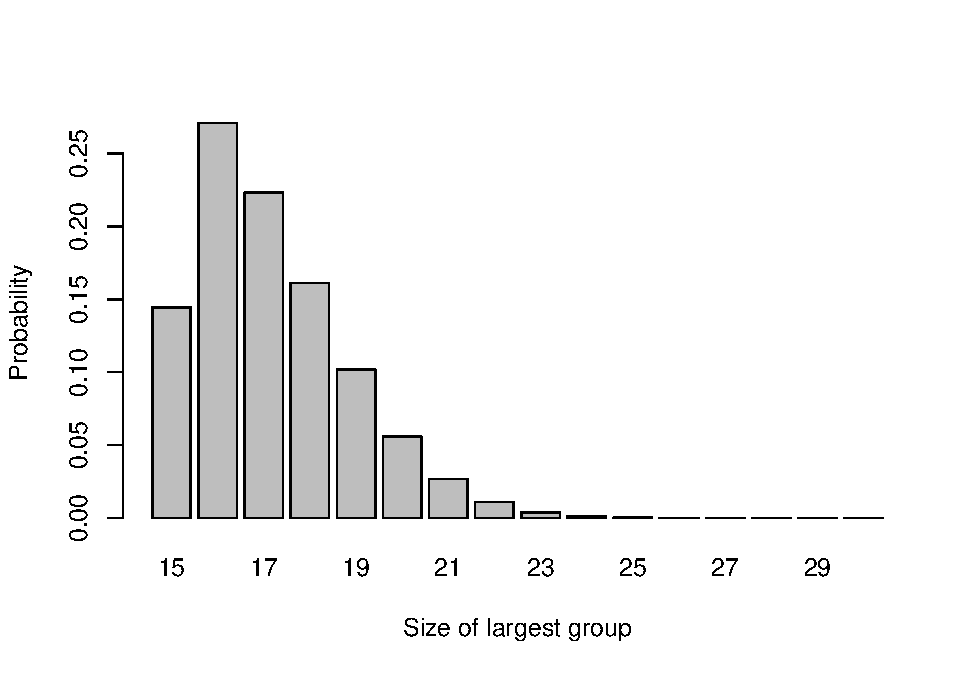
\includegraphics{CT4H_notes_files/figure-latex/srs-alloc-1.pdf}
\caption{\label{fig:srs-alloc}The probability distribution of largest group size for n=15.}
\end{figure}

As we have seen when thinking about sample sizes in Section \ref{sec-power}, this will reduce the power \(\Psi\) of the trial, since it depends on \(\lambda\left(N_C,\,N_T\right) = \sqrt{\frac{1}{N_C} + \frac{1}{N_T}}\).

For larger trials, this imbalance will be less pronounced, for example Figure \ref{fig:srsalloc200} shows the same for \(n=200\).

\begin{figure}
\centering
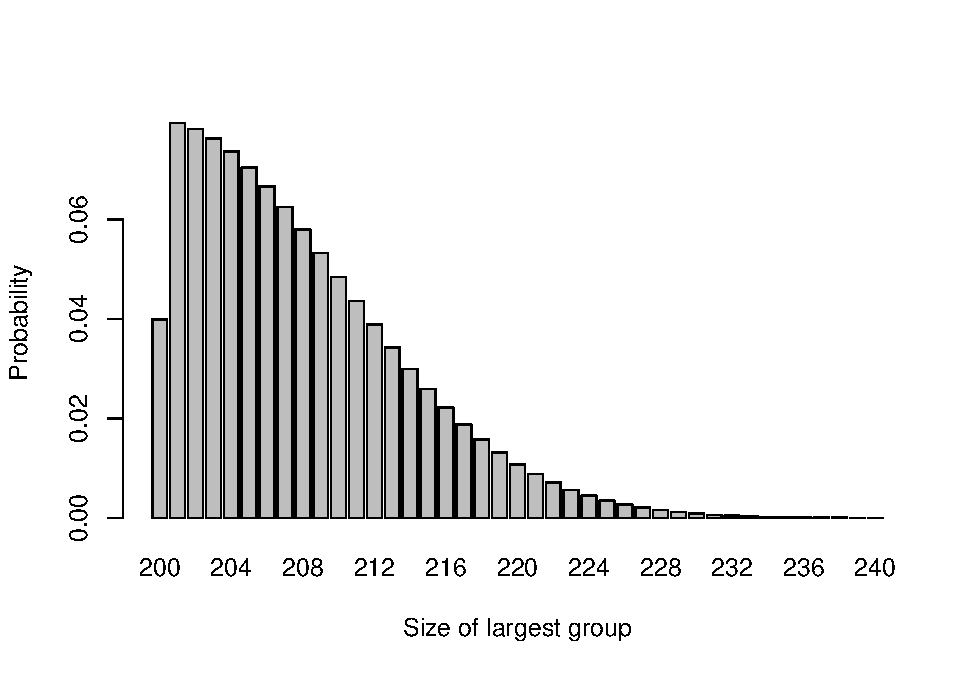
\includegraphics{CT4H_notes_files/figure-latex/srsalloc200-1.pdf}
\caption{\label{fig:srsalloc200}The probability distribution of largest group size for n=200.}
\end{figure}

In this case the \(P\left(N_{max} \geq 220\right)=0.051\), so the chance of highly imbalanced groups is much lower. However, we may want to achieve balance on some factor thought to be important, for example sex, age group or disease state, and in this case there may be small numbers even in a large trial.

We saw in the sample size section that the greatest power is achieved when group sizes are equal, since this minimises the function

\[\lambda\left(n,m\right) = \sqrt{\frac{1}{n}+\frac{1}{m}}.\]
However, with simple random sampling we can't guarantee equal group sizes.

\begin{example}
Suppose we are designing a trial to have \(\alpha=0.05\), and our minimum detectable effect size is such that \(\frac{\tau_M}{\sigma}=1\). If 30 participants are recruited, then we can calculate the power of the study using methods from Chapter 2:

\[1-\beta = \Phi\left(\sqrt{\frac{n_T\,n_C}{30}} - 1.96\right). \]
The first term in the standard normal CDF comes from the fact that

\[\left[\lambda\left(n,m\right)\right]^{-1} = \sqrt{\frac{nm}{n+m}} .\]
If we have equal group sizes \(n_T=n_C=15\), then the power achieved is 78\%.
If the group sizes are 10 and 20, we have a power of 73\%.
If the group sizes are 6 and 24, the power goes down to 59\%.

So, as we saw when looking at power, we don't lose too much if the group sizes are 2:1, but a more pronounced imbalace has resulted in a much more noticeable loss. There may be other disadvantages to having such imbalance, for example increased costs, or a reduction in the amount of information gained about side effects. If this imbalance can be avoided, it should be.
\end{example}

\hypertarget{random-permuted-blocks}{%
\subsection{Random permuted blocks}\label{random-permuted-blocks}}

One commonly used method to randomly allocate participants while avoiding too much imbalance is to use \emph{random permuted blocks} (RPBs). If the blocks have size \(2m\), and there are two groups then there are \[\binom{2m}{m},\] but this method can be adapted to more than two groups and to unequal group size.

If we have two groups, \(A\) and \(B\), then there are six \emph{blocks} of length 4 containing two \(A\)s and two \(B\)s

\[
\begin{aligned}
1.& AABB\\
2.& ABAB\\
3.& ABBA\\
4.& BAAB\\
5.& BABA\\
6.& BBAA.
\end{aligned}
\]

We can also randomly generate a sequence of numbers from \(\left\lbrace 1, 2, 3, 4, 5, 6 \right\rbrace\), where each number has equal probability. This sequence will correspond to a sequence in \(A\) and \(B\) with four times the length. In this method, each patient is equally likely to receive \(A\) and \(B\), but there will never be a difference of more than two between the size of the two groups.

For example, suppose the sequence begins \(2,1,3,6,\ldots\). Replacing each number by its block, we have \(ABAB\;AABB\;ABBA\;BBAA\;\ldots\).

One serious disadvantage of this method is that if the block size is fixed, and the doctors involved in the trial know which participants have received which treatments (which is unavoidable in cases such as surgery), then the allocation for some patients can be perfectly predicted. This is true for the fourth in every block, and for the third and fourth if the first two were the same. This means that selection bias may be a problem in more than 25\% of participants, which is deemed unacceptable; indeed, it fails our second point about randomization.

\hypertarget{rpbs-with-random-block-length}{%
\subsubsection{RPBs with random block length}\label{rpbs-with-random-block-length}}

The issue above can be circumvented by not only randomly choosing from a selection of blocks, but also randomly choosing the length of the block. For example, there are
\[ \binom{6}{3} = 20\]
possible blocks of size 6. Instead of always selecting from the six possible 4-blocks, a sampling scheme can be as follows.

\begin{enumerate}
\def\labelenumi{\arabic{enumi}.}
\tightlist
\item
  A random number \(X\) is drawn from \(\left\lbrace 4,6\right\rbrace\) to select the block length.
\item
  A second random number \(Y\) is drawn from 1 to 6 (if the block length is four) or 1 to 20 (if the block length is 6).
\item
  The block corresponding to \(Y\) is chosen and participants assigned accordingly.
\item
  If more participants are needed, go back to step 1.
\end{enumerate}

As well as ensuring that patients are equally likely to receive treatments \(A\) and \(B\), and that \(N_A\) and \(N_B\) can never differ by more than three, this method hugely reduces the possibility of enabling selection bias. The assignment of a patient can only be perfectly predicted if the difference is three, and this happens only for two of the twenty blocks of length six.

\hypertarget{bcurn}{%
\subsection{Biased coin designs and urn schemes}\label{bcurn}}

It may be that we prefer a method which achieves balance while retaining the pure stochasticity of simple random sampling. An advantage of RPBs was that once the sequence was generated, no computing power was needed. However, it is safe now to assume that any hospital pharmacy, nurse's station, GP office or other medical facility will have a computer with access to the internet (or some internal database), and therefore more sophisticated methods are available. It is also very likely that all trial data may be stored on some central database, and so methods that rely on knowing the allocation so far (albeit in some encrypted form) should be possible even if there are multiple clinicians and sites involved.

Biased coin designs and urn schemes both work by adjusting the probabilities of allocation according to balance of the design so far, such that a participant is less likely to be assigned to an over-represented group.

\hypertarget{biased-coin-designs}{%
\subsubsection{Biased coin designs}\label{biased-coin-designs}}

The biased coin design was introduced by \citet{efron1971forcing}, with the aim of ensuring balance whilst not becoming vulnerable to various forms of experimental bias. \citet{efron1971forcing} suggested the biased coin design be used within categories (eg. age group, sex, disease state etc.), but in this section we will think about the whole cohort (the maths for a subgroup would be the same).

Suppose we are using a biased coin design for a trial to compare two treatments, \(T\) and \(C\). At the point where some number \(n\) (not the total trial cohort) have been allocated, we can use the notation \(N_T\left(n\right)\) for the number of participants allocated to treatment \(T\), and \(N_C\left(n\right)\) for the number of participants allocated to treatment \(C\). Using these, we can denote the \emph{imbalance} in treatment numbers by

\[ D\left(n\right) = N_T\left(n\right) - N_C\left(n\right) = 2N_T\left(n\right) - n.\]
We use the imbalance \(D\left(n\right)\) to alter the probability of allocation to each treatment in order to restore (or maintain) balance in the following way:

\begin{itemize}
\tightlist
\item
  If \(D\left(n\right)=0\), allocate patient \(n+1\) to treatment \(T\) with probability \(\frac{1}{2}\).
\item
  If \(D\left(n\right)<0\), allocate patient \(n+1\) to treatment \(T\) with probability \(P\).
\item
  If \(D\left(n\right)>0\), allocate patient \(n+1\) to treatment \(T\) with probability \(1-P\).
\end{itemize}

where \(P\in\left(\frac{1}{2}, 1\right)\).

\begin{quote}
Question: What would happen if \(P=\frac{1}{2}\) or \(P=1\)?
\end{quote}

If, at some point in the trial, we have \(\lvert D\left(n\right)\rvert = j\), for some \(j>0\), then we must have either

\[ \lvert D\left(n+1\right)\rvert = j+1 \]
or
\[ \lvert D\left(n+1\right)\rvert = j-1 .\]
Because of the way we have set up the scheme,

\[ p\big(\lvert D\left(n+1\right)\rvert = j+1\big) = 1-P \]
and

\[ p\big(\lvert D\left(n+1\right)\rvert = j-1\big) = P.\]
If \(\lvert D\left(n\right) \rvert = 0\), ie. the scheme is in exact balance after \(n\) allocations, then we must have \(\lvert D\left(n\right)\rvert = 1\).

The absolute imbalances therefore form a simple random walk on the non-negative integers, with transition probabilities

\[
  \begin{aligned}
P\bigg(\lvert D\left(n+1\right) \rvert = 1 \; \bigg| \;\lvert D\left(n\right)\rvert=0\bigg)& = 1\\
P\bigg(\lvert D\left(n+1\right) \rvert = j+ 1 \; \bigg| \; \lvert D\left(n\right)\rvert=j\bigg)& = 1 - P\\
P\bigg(\lvert D\left(n+1\right) \rvert = j-1 \; \bigg| \; \lvert D\left(n\right)\rvert=j\bigg)& = P
\end{aligned}
\]
Figure \ref{fig:biasedcoin-p2thirds} shows four realisations of this random walk with \(P=0.667\) (Efron's preferred value). We see that sometimes the imbalance gets quite high, but in general it isn't too far from 0.

\begin{figure}
\centering
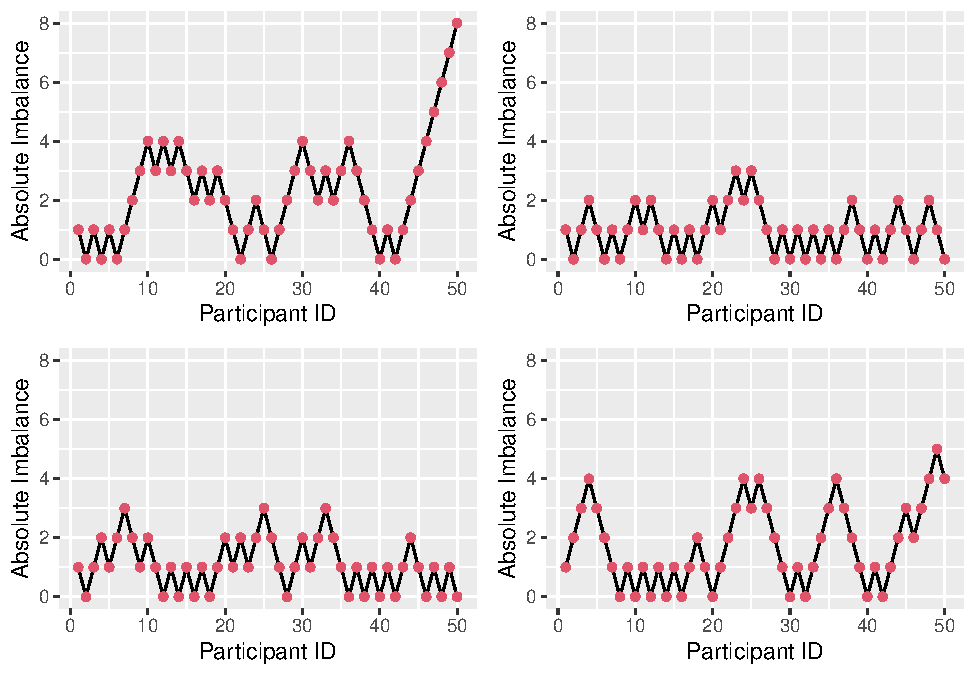
\includegraphics{CT4H_notes_files/figure-latex/biasedcoin-p2thirds-1.pdf}
\caption{\label{fig:biasedcoin-p2thirds}Absolute imbalance for a biased-coin scheme with \(P=0.667\).}
\end{figure}

Figure \ref{fig:p-nearlyhalf} shows four realisations of the random walk with \(P=0.55\). Here, the imbalance is able to get very high (note the change in \(y\)-axis); for example in the first plot, if we stopped the trial at \(n=50\) we would have 34 participants in one arm and only 16 in the other.

\begin{figure}
\centering
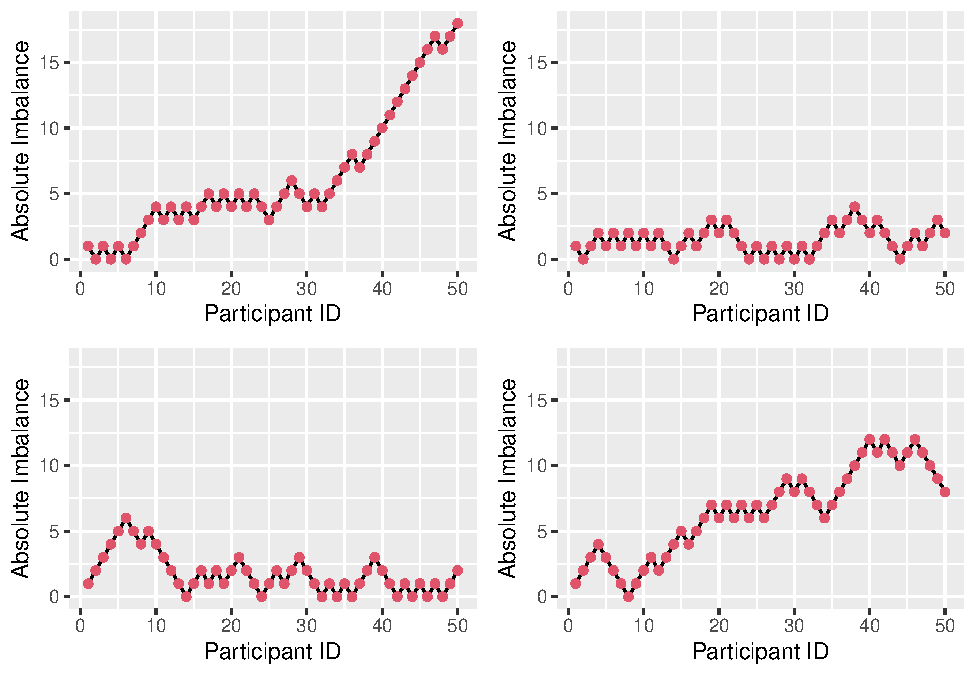
\includegraphics{CT4H_notes_files/figure-latex/p-nearlyhalf-1.pdf}
\caption{\label{fig:p-nearlyhalf}Absolute imbalance for a biased-coin scheme with \(P = 0.55\).}
\end{figure}

By contrast, with \(P=0.9\) as in Figure \ref{fig:p-nearlyone}, there is much less imbalance. However, this brings with it greater predictability. Although allocation is always random, given some degree of imbalance (likely to be known about by those executing the trial), the probability of guessing the next allocation correctly is high (0.9). This invites the biases we have been trying to avoid, albeit in an imperfect form.

\begin{figure}
\centering
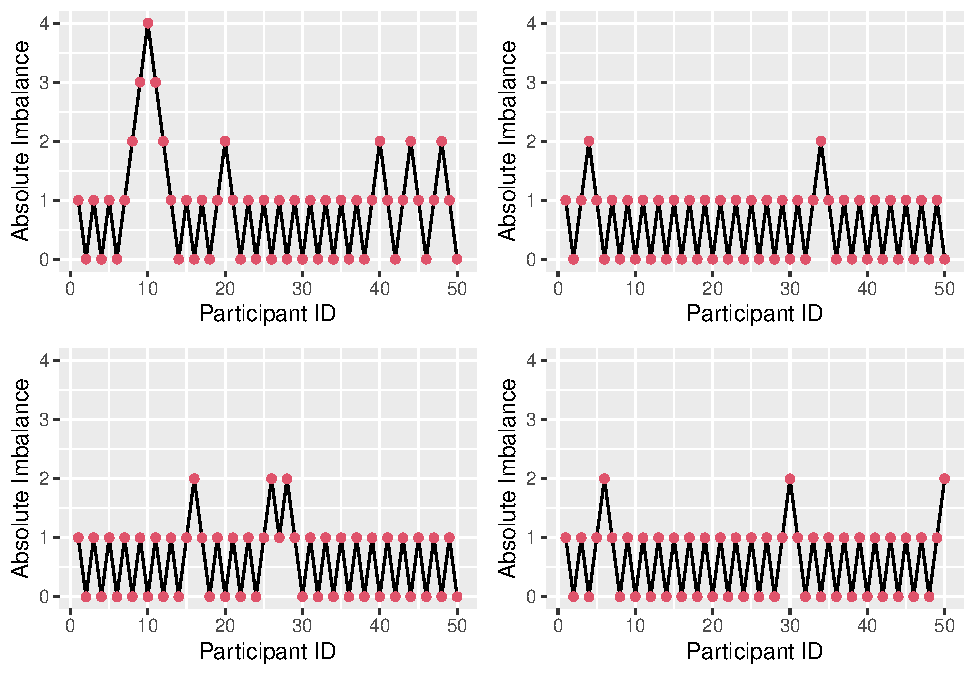
\includegraphics{CT4H_notes_files/figure-latex/p-nearlyone-1.pdf}
\caption{\label{fig:p-nearlyone}Absolute imbalance for a biased-coin scheme with \(P = 0.9\).}
\end{figure}

Efron's suggestion for implementation was that each clinician would received an unordered stack of envelopes. Each would contain three more envelopes, each with instructions covering one of the three possible cases (\(\lvert D\left(n\right)\rvert<0,\,\lvert D\left(n\right)\rvert=0\) and \(\lvert D\left(n\right)\rvert>0\)). The clinician would open the appropriate envelope and implement the instruction. Remember this was 1971!

A big disadvantage to the biased coin scheme is that the same probability is used regardless of the size of the imbalance (assuming it isn't zero). In the next section, we introduce a method where the probability of allocating the next patient to the underrepresented treatment gets larger as the imbalance grows.

\hypertarget{urn-models}{%
\subsubsection{Urn models}\label{urn-models}}

\emph{Urn models} for treatment allocation use urns in the way that you might well remember from school probability (or indeed often we had drawers of socks). They were first applied to clinical trials by \citet{wei1978application}. In this setting, the urn starts off with a ball for each treatment, and a ball is added to the urn each time a participant is allocated. The ball is labelled according to the treatment allocation that participant \textbf{did not} receive.

To allocate the next participant, a ball is drawn from the urn. If the allocations at this point are balanced, then the participant has equal probability of being allocated to each treatment. If there is imbalance, there will be more balls labelled by the underrepresented treatment, and so the participant is more likely to be allocated to that one. The greater the imbalance, the higher the probability of reducing it.

The process described so far is a \(UD\left(1,1\right)\); there is one ball for each treatment to start with, and one ball is added to the urn after each allocation. To be more general, we can assume a \(UD\left(r,s\right)\) scheme. Now, there are \(r\) balls for each treatment in the urn to begin with, and \(s\) are added after each allocation.

Near the start of the allocation, the probabilities are likely to change a lot to address imbalance, but once a `reasonable number' of allocations have been made it is likely to settle into simple random sampling (or very close).

Once again, we can find the transition probabilities by considering the absolute imbalance \(\lvert D\left(n\right) \rvert\).

Suppose that after participant \(n\), \(N_T\left(n\right)\) participants have been allocated to group \(T\), and \(N_C\left(n\right) = n - N_T\left(n\right)\) to group \(C\). The imbalance is therefore

\[D\left(n\right) = N_T\left(n\right) - N_C\left(n\right) = 2N_T\left(n\right) - n.\]
After \(n\) allocations there will be \(2r + ns\) balls in the urn: \(r\) for each treatment at the start, and \(s\) added after each allocation. Of these, \(r + N_C\left(n\right)s\) will be labelled by treatment \(T\) and \(r + N_T\left(n\right)s\) by treatment \(C\).

To think about the probabilities for the absolute imbalance \(\lvert D\left(n\right)\rvert\), we have to be careful now about which direction it is in. If the trial currently (after allocation \(n\)) has an imbalance of participants in favour of treatment \(C\), then the probability that it becomes less imbalanced at the next allocation is the probability of the next allocation being to treatment \(T\), which is

\[
  \begin{aligned}
p\left(\lvert D\left(n+1\right)\rvert = j-1 \mid D\left(n\right)=j, j>0\right) & = \frac{r + N_C\left(n\right)s}{2r + ns} \\
& = \frac{r + \frac{1}{2}\left(n + D\left(n\right)\right)s}{2r + ns} \\
& = \frac{1}{2} + \frac{D\left(n\right)s}{2\left(2r + ns\right)} \\
& = \frac{1}{2} + \frac{\lvert D\left(n\right)\rvert s}{2\left(2r + ns\right)}.
\end{aligned}
\]
Similarly, if there is currently an excess of patients allocated to treatment \(T\), then the imbalance will be reduced if the next allocation is to treatment \(C\), and so the conditional probability is

\[
  \begin{aligned}
p\left(\lvert D\left(n+1\right)\rvert = j-1 \mid D\left(n\right)=j, j<0\right) & = \frac{r + N_T\left(n\right)s}{2r + ns} \\
& = \frac{r + \frac{1}{2}\left(n - D\left(n\right)\right)s}{2r + ns} \\
& = \frac{1}{2} - \frac{D\left(n\right)s}{2\left(2r + ns\right)}\\
& = \frac{1}{2} + \frac{\lvert D\left(n\right)\rvert s}{2\left(2r + ns\right)}.
\end{aligned}
\]

Because the process is symmetrical, an imbalance of a given magnitude (say \(\lvert D\left(n\right)\rvert=j\)) is equally likely to be in either direction. That is

\[p\big(D\left(n\right) < 0 \mid \lvert D\left(n\right)\rvert =j \big)= p\big(D\left(n\right) > 0 \mid \lvert D\left(n\right)\rvert =j \big) = \frac{1}{2}.\]

Therefore we can use the law of total probability (or partition theorem) to find that

\[
  p\big(\lvert D\left(n+1\right) \rvert = j-1 \mid \lvert D\left(n\right) \rvert = j \big) = \frac{1}{2}  + \frac{\lvert D\left(n\right)\rvert s}{2\left(2r + ns\right)}.
\]
Since the two probabilities are equal this is trivial. Since the only other possibility is that the imbalance is increased by one, we also have

\[p\big(\lvert D\left(n+1\right) \rvert = j+1 \mid \lvert D\left(n\right) \rvert = j \big) = \frac{1}{2}  - \frac{\lvert D\left(n\right)\rvert s}{2\left(2r + ns\right)}. \]
As with the biased coin design, we also have the possibility that the imbalance after \(n\) allocations is zero, in which case the absolute imbalance after the next allocation will definitely be one. This gives us another simple random walk, with

\[
  \begin{aligned}
P\big(\lvert D\left(n+1\right) \rvert = 1 \mid \lvert D\left(n\right)=0\big)& = 1\\
P\big(\lvert D\left(n+1\right) \rvert = j+ 1 \mid \lvert D\left(n\right)=j\big)& = \frac{1}{2}  - \frac{\lvert D\left(n\right)\rvert s}{2\left(2r + ns\right)}\\
P\big(\lvert D\left(n+1\right) \rvert = j-1 \mid \lvert D\left(n\right)=j\big)& = \frac{1}{2}  + \frac{\lvert D\left(n\right)\rvert s}{2\left(2r + ns\right)}
\end{aligned}
\]

\begin{figure}
\centering
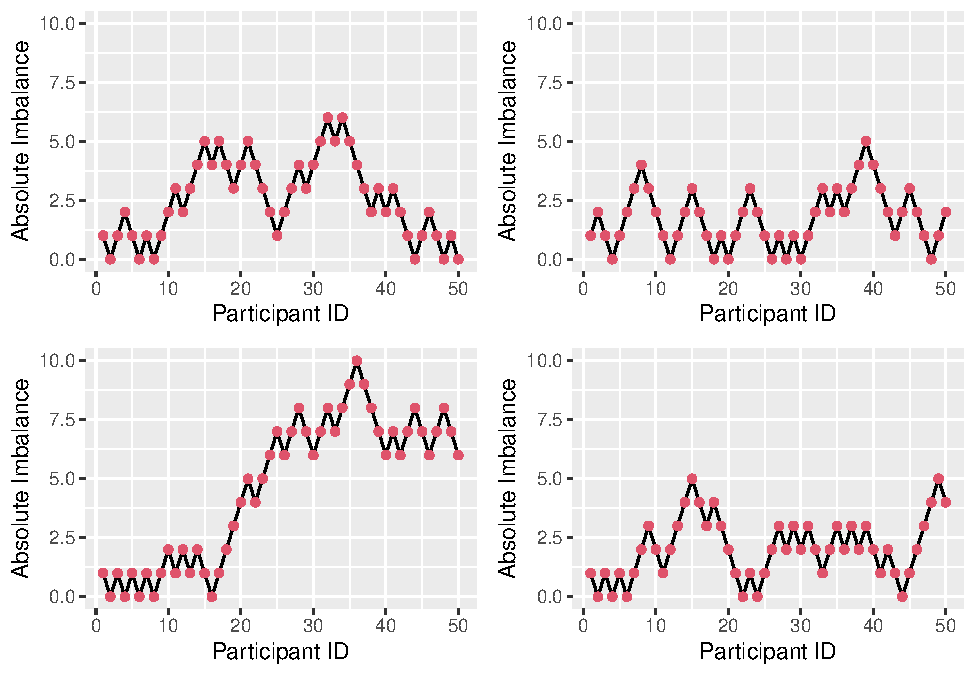
\includegraphics{CT4H_notes_files/figure-latex/urn11-1.pdf}
\caption{\label{fig:urn11}Four realisations of absolute imbalance for r=1, s=1, N=50.}
\end{figure}

\begin{figure}
\centering
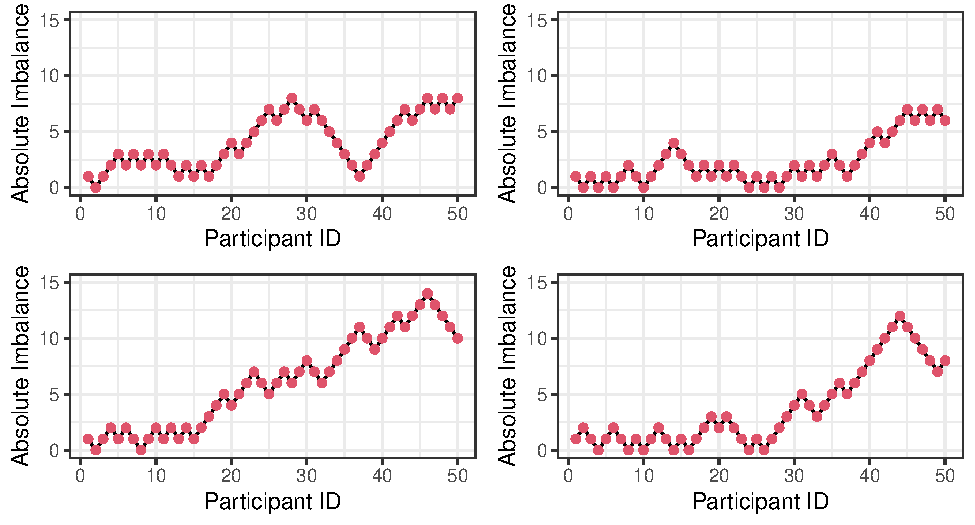
\includegraphics{CT4H_notes_files/figure-latex/urn18-1.pdf}
\caption{\label{fig:urn18}Four realisations of absolute imbalance for r=1, s=8, N=50.}
\end{figure}

\begin{figure}
\centering
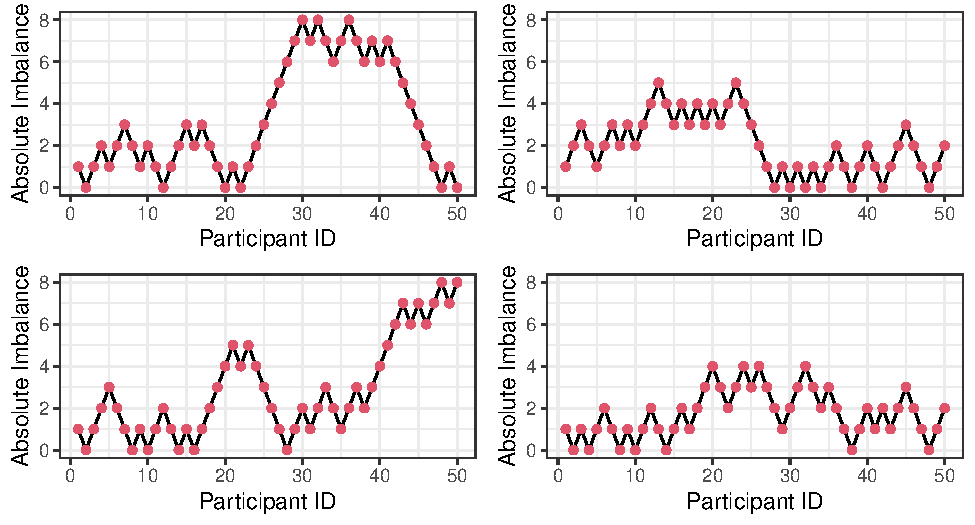
\includegraphics{CT4H_notes_files/figure-latex/urn81-1.pdf}
\caption{\label{fig:urn81}Four realisations of absolute imbalance for r=8, s=1, N=50.}
\end{figure}

We see that imbalance is reduced, particularly for small \(n\). A small \(r\) and large \(s\) enhance this, since the large number (\(s\)) of balls added to the urn with each allocation weight the probabilities more heavily, as in Figure \ref{fig:urn18}. By contrast, if \(r\) is large and \(s\) is small, as in Figure \ref{fig:urn81}, the probabilities stay closer to \(\left(\frac{1}{2}, \frac{1}{2}\right)\) and so more imbalance occurs early on.

\hypertarget{incorporating-baseline-measurements}{%
\section{Incorporating baseline measurements}\label{incorporating-baseline-measurements}}

At the start of the trial (ideally before allocation) various baseline measurements are usually taken. If the primary outcome variable is a continuous measurement (eg. blood pressure, weight,\ldots) this same quantity will often be included, so that there is some measure of each participant's condition/symptoms at the start of the trial. Factors such as age, sex, level of symptoms, things to do with treatment history and many others are included. Essentially, we include any variable we can that may lead to bias if not properly dealt with. The crucial thing is that none of these measurements (taken when they are) should be affected by the trial.

Such baseline measurements can be used in allocation.

\hypertarget{stratified-sampling}{%
\section{Stratified sampling}\label{stratified-sampling}}

The usual method of achieving balance with respect to prognostic factors is to divide each factor into several levels and to consider treatment assignment separately for patients having each particular combination of such factor levels. Such groups of patients are commonly referred to as randomization groups or strata. Treatment assignment is performed entirely separately for each stratum, a permuted block design of the type mentioned above often being used. In fact, using purely random treatment assignment for each stratum is equivalent to simple random assignment, so that some equalization of treatment numbers within each stratum is essential. Both the biased coin design and the urn design were intended for use in this way, adjusting in relation to imbalance within each stratum independently. This whole procedure is analogous to performing a factorial experiment, without being able to control the factor levels of the experimental units.

\begin{example}
Suppose we are planning a trial involving people over the age of 50, and we anticipate that age and sex might both play an important role in how participants respond to the treatment.

For sex, we use the levels `male' and `female', and for age we split the range into 50-65, 66-80 and 81 or over. We therefore have six strata, and we use an allocation strategy independently in each stratum. For example, below we have used randomly permuted blocks of length four.

\begin{tabular}{>{}l|l|l}
\hline
  & Male & Female\\
\hline
\textbf{50-65} & ABAB BBAA ... & ABBA BBAA ...\\
\hline
\textbf{66-80} & BAAB AABB ... & BABA BAAB ...\\
\hline
\textbf{81 and over} & ABAB ABBA ... & ABBA BAAB ...\\
\hline
\end{tabular}

Each time a new participant arrives, we follow the randomization pattern for their stratum. We could use another allocation scheme within each stratum, for example an urn model or a biased coin. It is important that we use one that aims to conserve balance, or else the benefits of stratification are lost.
\end{example}

A difficulty with stratified sampling is that the number of strata can quickly become large as the number of factors (or the number of levels within some factors) increases. For example, if we have four prognostic factors each with three levels, there are \(3^4=81\) strata. This creates a situation that is at best unwieldy, and at worst completely unworkable; in a small trial (with say 100 patients in each arm) there may be some strata with no patients in (this is actually not a problem), and probably many more with only one (this is much more problematic).

\hypertarget{minimization}{%
\section{Minimization}\label{minimization}}

Minimization was first proposed by \citet{taves1974minimization}, then shortly after by \citet{pocock1975sequential} and \citet{freedman1976use}. The aim of minimization is to minimize the difference between the two groups. It was developed for use with strata, as an alternative to randomly permuted blocks. Although the method was developed in the seventies, it has only gained popularity relatively recently, mainly as computers have become widely available.

To form the strata, the people running the trial must first specify all of the factors they would like to be balanced between the two groups. These should be any variables that are thought to possibly affect the outcome.

\begin{example}
The study by \citet{kallis1994pre} investigates the effect of giving aspirin to patients before coronary artery surgery with giving them a placebo. Interestingly, the effects of aspirin were found to be both positive (decreases platelet aggregation to arachidonic acid and to collagen) and negative (increased likelihood of post-operative excessive blood loss).
For their prognostic factors, \citet{kallis1994pre} chose age (\(\leq{50}\) or \(50\)), sex (M or F), operating surgeon (3 possibilities) and number of coronary arteries affected (1 or 2). This creates 24 strata. The trial had 100 participants, meaning an average of 4.17 in each stratum.
\end{example}

When a patient enters the trial, their level of each factor is listed. The patient is then allocated in such a way as to minimise any difference in these factors between the two groups. The minimization method has evolved since its conception, and exists in several forms. Two areas in which methods vary are

\begin{itemize}
\tightlist
\item
  Whether continuous variables have to be binned
\item
  Whether there is any randomness
\end{itemize}

It is generally agreed that if the risk of selection bias cannot be avoided, there should be an element of randomness. It is also usually accepted that if a variable is included in the minimization, it should also be included in the statistical analysis.

\hypertarget{minimization-algorithm}{%
\subsection{Minimization algorithm}\label{minimization-algorithm}}

Suppose we have a trial in which patients are recruited sequentially and need to be allocated to a trial arm (of which there are two). \citet{pocock1975sequential} give an algorithm in the general case of \(N\) treatment arms, but we will not do that here.

Suppose there are several prognostic factors over which we require balance, and that these factors have \(I, J, K, ...\) levels. In our example above, there would be \(I=2,\; J=2,\; K=3,\; L=2\). Note that this equates to 24 strata.

At some point in the trial, suppose we have recruited \(n_{ijkl}\) patients with levels \(i,\,j,\,k,\,l\) of the factors. For example, this may be males, aged over 50, assigned to the second surgeon, with both coronary arteries affected. Within these, \(n^A_{ijkl}\) have been assigned to treatment arm \(A\), and \(n^B_{ijkl}\) to arm \(B\). So we have

\[ n^A_{ijkl} + n^B_{ijkl} = n_{ijkl} .\]

If we were to use random permuted blocks within each stratum, then we would be assured that

\[\lvert n^A_{ijkl} - n^B_{ijkl} \rvert \leq{\frac{1}{2}b},\]
where \(b\) is the block length. However, there are two issues with this:

\begin{itemize}
\tightlist
\item
  There may be very few patients in some strata, in which case RPBs will fail to provide adequate balance.
\item
  It is unlikely that we actually need this level of balance.
\end{itemize}

The first point is a pragmatic one - the method usually guaranteed to achieve good balance is likely to fail, at least for some strata. The second is more theoretical. In general, we require that groups be balanced according to each individual prognostic factor, but not to interactions. For example, it is often believed that younger patients would have generally better outcomes, but that other factors do not systematically affect this difference.

Therefore, it is enough to make sure that the following are all small:

\[
\begin{aligned}
\lvert n^A_{i+++} - n^B_{i+++} \rvert&\text{ for each }i=1,\ldots,I\\
\lvert n^A_{+j++} - n^B_{+j++} \rvert&\text{ for each }j=1,\ldots,J\\
\ldots&
\end{aligned}
\]
where \(+\) represents summation over the other factors, so that for example

\[n^A_{++k+} = \sum\limits_{i,j,l}{n^A_{ijkl}}\]
is the total number of patients with level \(k\) of that factor assigned to treatment arm \(A\).

Therefore, instead of having \(IJKL\) constraints constraints, as we would with using randomly permuted blocks within each stratum, we have \(I+J+K+L\) constraints, one for each level of each factor. In our example this is 9 constraints rather than 24.

In order to implement minimisation, we follow these steps:

\begin{enumerate}
\def\labelenumi{\arabic{enumi}.}
\tightlist
\item
  Allocate the first patient by simple randomisation.
\item
  Suppose that at some point in the trial we have recruited \(n_{ijkl}\) patients with prognostic factors \(i,\,j,\,k,\,l\). Of these \(n^A_{ijkl}\) are allocated to treatment arm \(A\) and \(n^B_{ijkl}\) to arm \(B\).
\item
  A new patient enters the trial. They have prognostic factors at levels \(w,\,x,\,y,\,z\).
\item
  We form the sum
\end{enumerate}

\begin{equation}
  \left(n^A_{w+++} - n^B_{w+++}\right) + \left(n^A_{+x++} - n^B_{+x++}\right) + \left(n^A_{++y+} - n^B_{++y+}\right) + \left(n^A_{+++z} - n^B_{+++z}\right).
  \label{eq:minim}
  \end{equation}

\begin{enumerate}
\def\labelenumi{\arabic{enumi}.}
\setcounter{enumi}{4}
\tightlist
\item
  If the sum from step 4 is negative (that is, allocation to arm \(B\) as dominated up to now) then we allocate the new patient to arm \(A\) with probability \(P\), with \(P>0.5\). If the sum is positive, they are allocated to arm \(B\) with probability \(P\). If the sum is zero, they are allocated to arm \(A\) with probability \(\frac{1}{2}\).
\end{enumerate}

Some people set \(P=1\), whereas others would set \(\frac{1}{2}<P<1\) to retain some randomness. Although setting \(P=1\) makes the system deterministic, to predict the next allocation a doctor (or whoever) would need to know \(n^A_{i+++}\) and so on. This is very unlikely unless they are deliberately seeking to disrupt the trial. However, generally the accepted approach is becoming to set \(P<1\).

\begin{example}
\protect\hypertarget{exm:mustine}{}\label{exm:mustine}From \citet{altman1990practical} (citing \citet{fentiman1983control}).
In this trial, 46 patients with breast cancer were allocated to receive either Mustine (arm A) or Talc (arm B) as treatment for pleural effusions (fluid between the walls of the lung). They used four prognostic factors: age (\(\leq{50}\) or \(>50\)), stage of disease (I or II, III or IV), time in months between diagnosis of breast cancer and diagnosis of pleural effusions (\(\leq{30}\) or \(>30\)) and menopausal status (Pre or post).

Let's suppose that 15 patients have already been allocated. The totals of patients in each treatment arm in terms of each level of each prognostic factor are shown in Table \ref{tab:minimeg}.

\begin{table}

\caption{\label{tab:minimeg}Allocations of first 15 patients, divided by diagnostic factor}
\centering
\begin{tabular}[t]{>{}l|l|r|r}
\hline
factor & level & Mustine (A) & Talc (B)\\
\hline
\textbf{Age} & 1. 50 or younger & 3 & 4\\
\hline
\textbf{Age} & 2. >50 & 4 & 4\\
\hline
\textbf{Stage} & 1. I or II & 1 & 2\\
\hline
\textbf{Stage} & 2. III or IV & 6 & 6\\
\hline
\textbf{Time interval} & 1. 30 months or less & 4 & 2\\
\hline
\textbf{Time interval} & 2. >30 months & 4 & 5\\
\hline
\textbf{Menopausal status} & 1. Pre & 4 & 3\\
\hline
\textbf{Menopausal status} & 2. Post & 5 & 3\\
\hline
\end{tabular}
\end{table}

Suppose our sixteenth patient is under 50, has disease at stage III, has less than 30 months between diagnoses and is pre-menopausal.
Our calculation from step 4 of the minimisation algorithm is therefore

\[
\begin{aligned}
\left(n^A_{1+++} - n^B_{1+++}\right) + \left(n^A_{+2++} - n^B_{+2++}\right) + \left(n^A_{++1+} \right.& \left.- n^B_{++1+}\right) + \left(n^A_{+++1} - n^B_{+++1}\right) \\
& = \left(3-4\right) + \left(6-6\right) + \left(4-2\right) + \left(4-3\right) \\
& = -1 + 0 + 2 + 1\\
& = 2 .
\end{aligned}
\]
Since our sum is greater than zero, we allocate the new patient to arm B (talc) with some probability \(P\in\left(0.5,1\right)\) and update the table before allocating patient 17.
\end{example}

One shortcoming of minimisation is that the factors are equally weighted in the algorithm, regardless of the number of patients with that particular factor level. For example, suppose at some later stage of allocation in Example \ref{exm:mustine}, only four patients with stage I or II disease had been recruited, and that one of these had been allocated to group \(A\) and three to group \(B\). At the same point, 18 of the recruited number were post-menopausal, and of these 10 had been allocated to group \(A\) and 8 to group \(B\). The values contributed to the sum in Equation \eqref{eq:minim} are \(+2\) and \(-2\), so these imbalances effectively cancel one another out, but intuitively it would feel sensible to prioritise equal distribution within the stage I or II women, since proportionally this stratum is less balanced. \citet{wei1978application} proposed an extension of the Urn Design that does exactly this, but we won't cover this method in our course.

\hypertarget{problems-around-allocation}{%
\section{Problems around allocation}\label{problems-around-allocation}}

In clinical trials papers, the allocation groups are usually summarised in tables giving summary statistics (eg. mean and SD) of each characteristic for the control group and the intervention group. The aim of these is to show that the groups are similar enough for any difference in outcome to be attributed to the intervention itself. Figure \ref{fig:licorice-participants} shows an example, taken from \citet{ruetzler2013randomized}.

\begin{figure}
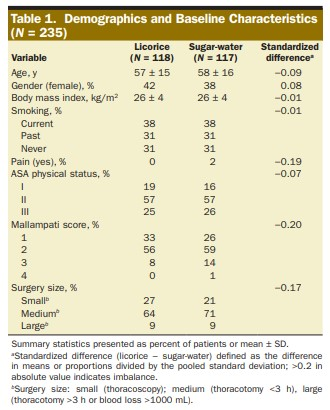
\includegraphics[width=0.6\linewidth]{images/licorice} \caption{Summary statistics for an RCT comparing a licorice gargle (the intervention) to a sugar-water gargle (the standard). From @ruetzler2013randomized}\label{fig:licorice-participants}
\end{figure}

The problem here is that only the marginal distributions are compared for similarity. Consider the following (somewhat extreme and minimalistic) scenario. A study aims to investigate the effect of some treatment, and to balance for gender and age in their allocation, resulting in the following summary table.

\begin{tabular}{>{}l|l|l}
\hline
  & Male & Female\\
\hline
\textbf{Control} & 57.51 (7.09) & 40.31 (5.83)\\
\hline
\textbf{Intervention} & 44.19 (5.96) & 60.03 (5.27)\\
\hline
\end{tabular}

This appears to be a reasonably balanced design. However, if we look at the joint distribution, we see that there are problems.

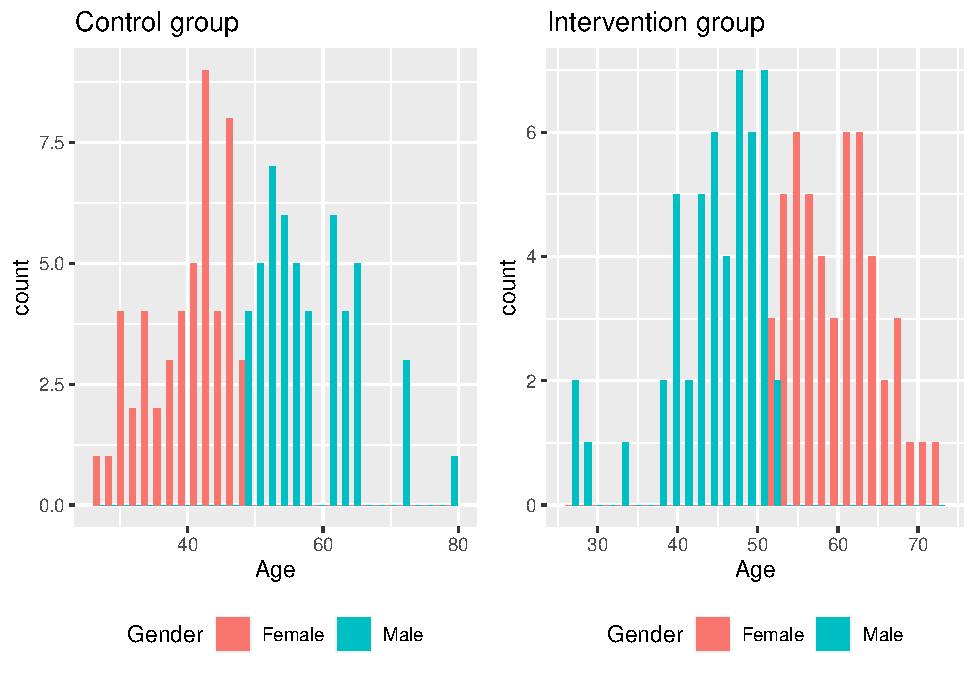
\includegraphics{CT4H_notes_files/figure-latex/unnamed-chunk-10-1.pdf}

If the intervention is particularly effective in older men, our trial will not notice. Likewise, if older women generally have a more positive outcome than older men, our trial may erroneously find the intervention to be effective.

Although this example is highly manufactured and {[}hopefully!{]} unlikely to take place in real life, for clinical trials there are often many demographic variables and prognostic factors being taken into account. Achieving joint balance across all them is very difficult, and extremely unlikely to happen if it isn't aimed for. \citet{treasure1998minimisation} give an example in relation to a hypothetical study on heart disease

\begin{quote}
Supposing one group has more elderly women with diabetes and symptoms of heart failure. It would then be impossible to attribute a better outcome in the other group to the beneficial effects of treatment since poor left ventricular function and age at outset are major determinants of survival in any longitudinal study of heart disease, and women with diabetes, as a group, are likely to do worse. At this point the primary objective of randomisation---exclusion of confounding factors---has failed. \ldots{} If a very big trial fails, because, for example, the play of chance put more hypertensive smokers in one group than the other, the tragedy for the trialists, and all involved, is even greater.
\end{quote}

However, this issue is rarely addressed in clinical trials: a lot of faith is placed (with reasonable justification) in the likely balance achieved by random sampling, whatever method is used. We will also see in the next Chapter that we can account for some degree of imbalance at the analysis stage.

\hypertarget{rct-analysis}{%
\chapter{Analyzing RCT data}\label{rct-analysis}}

We're now in the post-trial stage. The trial has been run, and we have lots of data to analyze to try to assess what effect the treatment or intervention has had. In general we will use the notation \(\tau\) to denote the treatment effect.

In this chapter we'll keep our focus on the scenario where the trial outcome is measured on a continuous scale, but in later weeks we'll go on to look at other types of data.

\begin{example}
To illustrate the theory and methods, we'll use an example dataset from \citet{hommel1986effect} (this example is also used by \citet{matthews2006introduction}). The data involves a trial of 16 diabetes patients, and focusses on a drug (Captopril) that may reduce blood pressure. This is important, since for those with diabetes, high blood pressure can exacerbate kidney disease (specifically diabetic nephropathy, a complication of diabetes). To participate in the trial, people had to be insulin-dependent and already affected by diabetic nephropathy. In the trial, systolic blood pressure was measured before participants were allocated to each trial arm, and then measured again after one week on treatment. A placebo was given to the control group, so that all participants were blinded.

The baseline and outcome blood pressure measurements (in mmHg) are shown in Table \ref{tab:captoprildata}. We see that nine participants were assigned to the treatment arm (Captopril) and the remaining seven to the placebo group. \citet{hommel1986effect} say that the patients were `randomly allocated' to their group.

\begin{table}

\caption{\label{tab:captoprildata}Data for the Captopril trial from @hommel1986effect.}
\centering
\begin{tabular}[t]{rrrl}
\toprule
Patient (ID) & Baseline (B) & Outcome at 1 week (X) & Trial Arm\\
\midrule
1 & 147 & 137 & Captopril\\
2 & 129 & 120 & Captopril\\
3 & 158 & 141 & Captopril\\
4 & 164 & 137 & Captopril\\
5 & 134 & 140 & Captopril\\
\addlinespace
6 & 155 & 144 & Captopril\\
7 & 151 & 134 & Captopril\\
8 & 141 & 123 & Captopril\\
9 & 153 & 142 & Captopril\\
1 & 133 & 139 & Placebo\\
\addlinespace
2 & 129 & 134 & Placebo\\
3 & 152 & 136 & Placebo\\
4 & 161 & 151 & Placebo\\
5 & 154 & 147 & Placebo\\
6 & 141 & 137 & Placebo\\
\addlinespace
7 & 156 & 149 & Placebo\\
\bottomrule
\end{tabular}
\end{table}

This is very small dataset, and so in that respect it is quite unusual, but its structure is similar to many other trials.
\end{example}

We will build up from the simplest type of analysis to some more complicated / sophisticated approaches.

\hypertarget{ttest}{%
\section{Confidence intervals and P-values}\label{ttest}}

Because the randomization process should produce groups that are comparable, we should in principle be able to compare the primary outcome (often referred to as \(X\)) between the groups.

\begin{example}
Summary statistics of the outcome for each group are shown below.

\begin{table}

\caption{\label{tab:unnamed-chunk-11}Summary statistics for each group.}
\centering
\begin{tabular}[t]{l|r|r|r|r}
\hline
  & Sample Size & Mean (mmHg) & SD (mmHg) & SE of mean (mmHg)\\
\hline
Captopril & 9 & 135.33 & 8.43 & 2.81\\
\hline
Placebo & 7 & 141.86 & 6.94 & 2.62\\
\hline
\end{tabular}
\end{table}

We see that the difference in mean outcome (systolic blood pressure) between the two groups is \(141.86 - 135.33 = 6.53 \text{mmHg}\). Clearly overall there has been some reduction in systolic blood pressure for those in the Captopril arm, but how statistically sound is this as evidence? It could be that really (for the hypothetical population) there is no reduction, and we have just been `lucky'.

The variances within the two groups are fairly close, so we can use the pooled estimate of standard deviation:

\[
  s_p = \sqrt{\frac{\sum\limits_{i=1}^N\left(n_i-1\right)s_i^2}{\sum\limits_{i-1}^N\left(n_i-1\right)}}.
\]

In our case

\[ 
  \begin{aligned}
s_p&= \sqrt{\frac{8\times{8.43^2} + 6 \times{6.94^2}}{8+6}}\\
& = 7.82\text{ mmHg.}
\end{aligned}
\]
This enables us to do an independent two-sample \(t\)-test, and we can find the \(t\) statistic

\[
  \begin{aligned}
t & = \frac{\bar{X_C} - \bar{X_T}}{s_p\sqrt{\frac{1}{n_C} + \frac{1}{n_T}}}\\
& = \frac{6.53}{7.82\sqrt{\frac{1}{7} + \frac{1}{9}}} \\
& = 1.65.
\end{aligned}
\]
Note that here the placebo group is group \(C\), and the Captopril group is group \(T\).

Under the null hypothesis that the mean systolic blood pressure at the end of the week of treatment/placebo is the same in both groups, this value should have a \(t\) distribution with 14 degrees of freedom (\(n_i-1\) for each group).

\begin{figure}
\centering
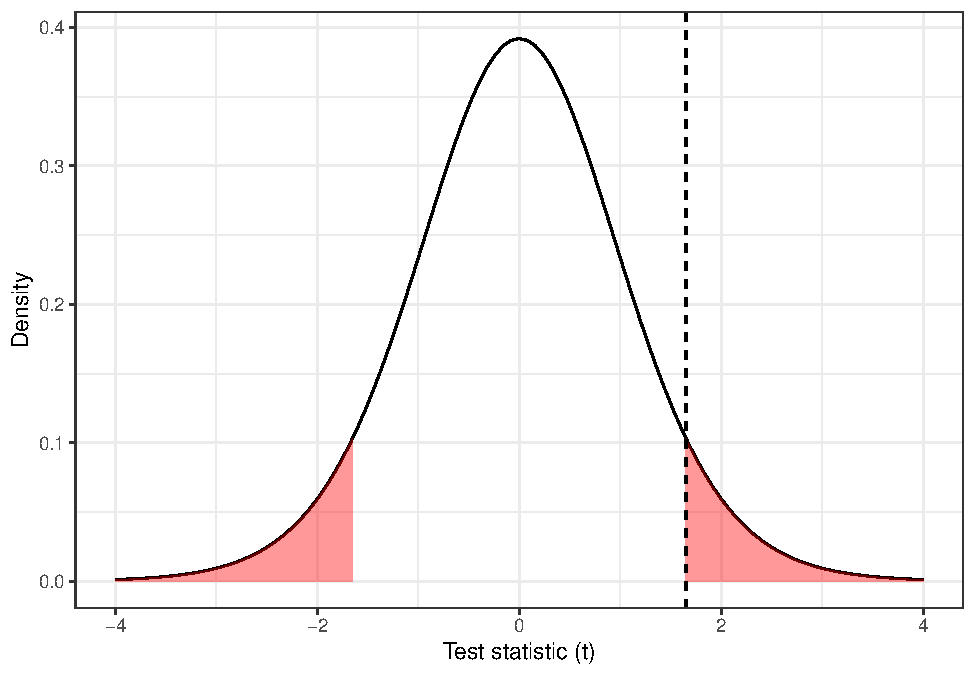
\includegraphics{CT4H_notes_files/figure-latex/ttestcapt-1.pdf}
\caption{\label{fig:ttestcapt}The distribution \(t_{14}\), with \(t=1.65\) shown by the dashed line and the `more extreme' areas shaded.}
\end{figure}

The dashed line in Figure \ref{fig:ttestcapt} is at \(t=1.65\), and the red shaded areas show anywhere `at least as extreme'. We can find the area (ie. the probability of anything at least as extreme as our found value) in R by

\begin{Shaded}
\begin{Highlighting}[]
\DecValTok{2}\SpecialCharTok{*}\NormalTok{(}\DecValTok{1}\SpecialCharTok{{-}}\FunctionTok{pt}\NormalTok{(}\FloatTok{1.65}\NormalTok{, }\AttributeTok{df=}\DecValTok{14}\NormalTok{))}
\end{Highlighting}
\end{Shaded}

\begin{verbatim}
## [1] 0.1211902
\end{verbatim}

This is the value we know as `the P value'. We see that in this case our results are not statistically significant (at the 0.10 level), under this model.
\end{example}

\hypertarget{what-do-we-do-with-this-outcome}{%
\subsection{What do we do with this outcome?}\label{what-do-we-do-with-this-outcome}}

The outcome of this Captopril study is in some ways the worst case scenario. The difference in means is large enough to be compelling, but our dataset is too small for it to be statistically significant, and so we can't confidently conclude that Captopril has any effect on blood pressure. However, we also can't say that there is no effect. This is exactly the sort of scenario we hoped to avoid when planning our study.

One way to reframe the question is to consider the range of treatment effects that are compatible with our trial data. That is, we find the set

\[\left\lbrace \tau \mid \frac{\lvert \bar{x}_C - \bar{x}_T - \tau \rvert}{s\sqrt{n_C^{-1} + n_T^{-1}}} \leq t_{n_C+n_T-2;\,0.975} \right\rbrace, \]
which contains all possible values of treatment effect \(\tau\) that are compatible with our data. That is, suppose the true treatment effect is \(\tau^*\), and we test the hypothesis that \(\tau = \tau^*\). For all values of \(\tau^*\) inside this range, our data are not sufficiently unlikely to reject the hypothesis at the 0.05 level. However, for all values of \(\tau^*\) outside this range, our data are sufficiently unlikely to reject that hypothesis. We can rearrange this to give a 95\% confidence interval for \(\tau\),

\[\left\lbrace \tau \mid \bar{x}_C - \bar{x}_T - t_{n_C+n_T-2;\,0.975}\,s\sqrt{n_C^{-1} + n_T^{-1}} \leq \tau \leq \bar{x}_C - \bar{x}_T + t_{n_C+n_T-2;\,0.975}\,s\sqrt{n_C^{-1} + n_T^{-1}}  \right\rbrace \]

\begin{example}
Continuing our example, we have

\[\left\lbrace \tau \mid \frac{\lvert 6.53 - \tau \rvert}{7.82\sqrt{\frac{1}{7} + \frac{1}{9}}} \leq t_{14;0.975} = 2.145 \right\rbrace \]

Here, \(t_{14;0.975} = 2.145\) is the \(t\)-value for a significance level of \(0.05\), so if we were working to a different significance level we would change this.

Rearranging as above, this works out to be the interval

\[
-1.92 \leq  \tau \leq 14.98.
\]

Notice that zero is in this interval, consistent with the fact that we failed to reject the null hypothesis.
\end{example}

Some things to note

\begin{itemize}
\tightlist
\item
  We can compute this confidence interval whether or not we failed to reject the null hypothesis that \(\tau=0\), and for significance levels other than 0.05.
\item
  In most cases, reporting the confidence interval is much more informative than simply reporting the \(P\)-value. In our Captopril example, we found that a negative treatment effect (ie. Captopril reducing blood pressure less than the placebo) of more than 2 mmHg was very unlikely, whereas a positive effective (Captopril reducing blood pressure) of up to 15 mmHg was plausible. If Captopril were inexpensive and had very limited side effects (sadly neither of which is true) it may still be an attractive drug.
\item
  These confidence intervals are exactly the same as you have learned before, but we emphasise them because they are very informative in randomised controlled trials (but not so often used!).
\end{itemize}

At the post trial stage, when we have data, the confidence interval is the most useful link to the concept of \emph{power}, which we thought about at the planning stage. Remember that the power function is defined as

\[\psi \left(\tau\right) = P\left(\text{Reject }H_0\mid \tau\neq 0\right),\] that is, the probability that we successfully reject \(H_0\) (that \(\tau=0\)) given that there is a non-zero treatment effect \(\tau\neq 0\). This was calculated in terms of the theoretical model of the trial, and in terms of some minimum detectable effect size \(\tau_M\) that we wanted to be able to correctly detect with probability \(1-\beta\) (the power). Sometimes people attempt to re-calculate the power after the trial, to detect whether the trial was underpowered. However, now we have actual data. If we failed to reject \(H_0\) and \(\tau_M\) is in the confidence interval for \(\tau\), then that is a good indication that our trial was indeed underpowered.

\hypertarget{baseline}{%
\section{Using baseline values}\label{baseline}}

In our example above, our primary outcome variable \(X\) was the systolic blood pressure of each participant at the end of the intervention period. However, we see in Table \ref{tab:captoprildata} that we also have \emph{baseline} measurements: measurements of systolic blood pressure for each patient from before the intervention period. Baseline measurements are useful primarily for two reasons:

\begin{enumerate}
\def\labelenumi{\arabic{enumi}.}
\tightlist
\item
  They can be used to assess the balance of the design.
\item
  They can be used in the analysis.
\end{enumerate}

We will demonstrate these by returning to our Captopril example.

\begin{example}
Firstly, we use the baseline systolic blood pressure to assess balance. The placebo group has a mean of 146.6 mmHg and an SD of 12.3 mmHg, whereas the Captopril group has mean 148.0 mmHg, SD 11.4 mmHg. While these aren't identical, they are sufficiently similar not to suspect any systematic imbalance. In a study this small there is likely to be some difference.

Secondly, since we are interested in whether the use of Captopril has reduced blood pressure for each individual, and these individuals had different baseline values, it makes sense to compare not just the outcome but the difference from baseline to outcome for each individual. We can see individual data in Table \ref{tab:captoprildiff} and summary statistics in Table \ref{tab:captoprildiffsumm}.

\begin{table}

\caption{\label{tab:captoprildiff}Data for the Captopril trial, with differences shown.}
\centering
\begin{tabular}[t]{r|r|r|l|r}
\hline
Patient (ID) & Baseline (B) & Outcome at 1 week (X) & Trial Arm & Difference\\
\hline
1 & 147 & 137 & Captopril & -10\\
\hline
2 & 129 & 120 & Captopril & -9\\
\hline
3 & 158 & 141 & Captopril & -17\\
\hline
4 & 164 & 137 & Captopril & -27\\
\hline
5 & 134 & 140 & Captopril & 6\\
\hline
6 & 155 & 144 & Captopril & -11\\
\hline
7 & 151 & 134 & Captopril & -17\\
\hline
8 & 141 & 123 & Captopril & -18\\
\hline
9 & 153 & 142 & Captopril & -11\\
\hline
1 & 133 & 139 & Placebo & 6\\
\hline
2 & 129 & 134 & Placebo & 5\\
\hline
3 & 152 & 136 & Placebo & -16\\
\hline
4 & 161 & 151 & Placebo & -10\\
\hline
5 & 154 & 147 & Placebo & -7\\
\hline
6 & 141 & 137 & Placebo & -4\\
\hline
7 & 156 & 149 & Placebo & -7\\
\hline
\end{tabular}
\end{table}

\begin{table}

\caption{\label{tab:captoprildiffsumm}Summary statistics for each group.}
\centering
\begin{tabular}[t]{l|r|r|r|r}
\hline
  & Sample Size & Mean (mmHg) & SD (mmHg) & SE of mean (mmHg)\\
\hline
Captopril & 9 & -12.67 & 8.99 & 3.00\\
\hline
Placebo & 7 & -4.71 & 7.91 & 2.99\\
\hline
\end{tabular}
\end{table}

Now we can perform our test as before, in which case we find

\[ t = \frac{-4.71 - (-12.67)}{8.54\sqrt{\frac{1}{7}+\frac{1}{9}}} = 1.850 \]
where 8.54 is the pooled standard deviation (as before). Under the null distribution of no difference, this has a \(t\)-distribution with 14 degrees of freedom, and so we have a \(P\)-value of 0.086. Our 0.95 confidence interval is

\[ -4.71 - (-12.67) \pm t_{14;\,0.975}\times 8.54\sqrt{\frac{1}{7}+\frac{1}{9}} = \left[-1.3,\,17.2\right].\]
We see that taking into account the baseline values in this way has slightly reduced the \(P\)-value and shifted the confidence interval slightly higher. Though at the \(\alpha = 0.05\) level we still don't have significance.
\end{example}

We will now look into why the confidence interval and \(P\)-value changed in this way, before going on to another way of taking into account the baseline value.

Let's label the baseline measurement for each group \(B_C\) and \(B_T\), and the outcome measurements \(X_C,\,X_T\), where we will take group \(C\) to be the placebo/control group and group \(T\) to be the treatment group. Because all participants have been randomised from the same population, we have

\[\operatorname{E}\left(B_C\right) = \operatorname{E}\left(B_T\right) = \mu_B.\]
Assuming some treatment effect \(\tau\) (which could still be zero) we have

\[
\begin{aligned}
\operatorname{E}\left(X_C\right) & = \mu\\
\operatorname{E}\left(X_T\right) & = \mu + \tau.
\end{aligned}
\]
Usually we will assume that

\[\operatorname{Var}\left(X_C\right) = \operatorname{Var}\left(X_T\right) = \operatorname{Var}\left(B_C\right) = \operatorname{Var}\left(B_T\right) = \sigma^2,\]
and this is generally fairly reasonable in practice.

Notice that for the two analyses we have performed so far (comparing outcomes and comparing differences) we have

\[
\begin{aligned}
\operatorname{E}\left(X_T\right) - \operatorname{E}\left(X_C\right) & = \left(\mu + \tau\right) - \mu = \tau\\
\operatorname{E}\left(X_T - B_T\right) - \operatorname{E}\left(X_C - B_C\right) & = \left(\mu - \mu_B + \tau\right) - \left(\mu - \mu_B\right) = \tau,
\end{aligned}
\]
that is, both are unbiased estimators of \(\tau\).

However, whereas the first is based on data with variance \(\sigma^2\), the second has

\[
\begin{aligned}
\operatorname{Var}\left(X_T-B_T\right) & = \operatorname{Var}\left(X_T\right) + \operatorname{Var}\left(B_T\right) - 2\operatorname{cov}\left(X_T,B_T\right)\\
& = \sigma^2 + \sigma^2 - 2\rho\sigma^2 \\
& = 2\sigma^2\left(1-\rho\right),
\end{aligned}
\]
where \(\rho\) is the true correlation between \(X\) and \(B\), and is assumed to be the same in either group. Similarly,

\[\operatorname{var}\left(X_C-B_C\right) = 2\sigma^2\left(1-\rho\right).\]
Using this to work out the variance of the estimator \(\hat{\tau}\) we find that for comparing means, assuming two equally sized groups of size \(N\), we have

\[\operatorname{var}\left(\hat{\tau}\right) = \operatorname{var}\left(\bar{x}_T - \bar{x}_C\right) = \frac{2\sigma^2}{N}.\]

whereas for comparing differences from baseline

\[\operatorname{var}\left(\hat{\tau}\right) = \operatorname{var}\left[\left(\overline{X_T-B_T}\right) - \left(\overline{X_C - B_C}\right)\right] = 2\left(1-\rho\right)\left(\frac{2\sigma^2}{N}\right).\]

Therefore, if \(\frac{1}{2}<\rho\leq 1\) there will be a smaller variance when comparing differences. However, if \(0\leq\rho<\frac{1}{2}\), the variance will be smaller when comparing outcome variables.

Intuitively, this seems reasonable: if the correlation between baseline and outcome measurements is very strong, then we can remove some of the variability between participants by taking into account their baseline measurement. However, if the correlation is weak, then by including the baseline in the analysis we are essentially just introducing noise.

For our Captopril example, the sample correlation between baseline and outcome is 0.63 in the Captopril group and 0.80 in the Placebo group. This fits with the \(P\)-value having reduced slightly.

\hypertarget{a-dodgy-way-to-use-baseline-variables}{%
\subsection{A dodgy way to use baseline variables}\label{a-dodgy-way-to-use-baseline-variables}}

Sometimes the analysis performed on a dataset is rather spurious, but it isn't always immediately obvious why. We'll look at one example now, because it is done sometimes.

This approach involves looking at each group separately, and determining whether there has been a significant change in the outcome variable (note that this only `works' if \(\mu_B = \mu\)).

For example, with our Captopril data, we could perform a paired \(t\)-test on the difference between baseline \(B\) and outcome \(X\) for each patient, for each group.

If we do this, we find the summary statistics in Table \ref{tab:ttestdodge}.

\begin{table}

\caption{\label{tab:ttestdodge}Summary statistics for the dodgy analysis}
\centering
\begin{tabular}[t]{l|r|r|r}
\hline
  & T statistic & Deg of freedom & P-value\\
\hline
Captopril & 4.23 & 8 & 0.003\\
\hline
Placebo & 1.58 & 6 & 0.170\\
\hline
\end{tabular}
\end{table}

From this we see that there is strong evidence for a change in blood pressure for the Captopril patients (group \(T\)), which isn't surprising, and no such evidence for the placebo patients. Can we therefore conclude that Captopril is significantly better than the placebo? No! The analysis is flawed:

\begin{itemize}
\tightlist
\item
  The \(p\)-value of 0.17 in the control group doesn't show that the null hypothesis (no treatment effect for the control group) is true, just that we can't reject the null hypothesis. It is quite possible that there is a difference in the control group, and that numerically it could even be comparable to that in the treatment group, so although we can say that there is a significant reduction in blood pressure for the captopril group, we can't conclude that Captopril is better than the placebo.
\item
  Having set up the experiment as a randomised controlled trial, with a view to comparing the two groups, it seems strange to then deal with them separately.
\end{itemize}

\hypertarget{analysis-of-covariance-ancova}{%
\section{Analysis of covariance (ANCOVA)}\label{analysis-of-covariance-ancova}}

In the previous section we based our analysis on the baseline values being statistically identical draws from the underlying distribution, and therefore having the same expectation and variance.

However, although this is theoretically true, in real life trials there will be some imbalance in the baseline measurements for the different treatment arms. We can see this in our Captopril example, in Figure \ref{fig:hommel}.

\begin{figure}
\centering
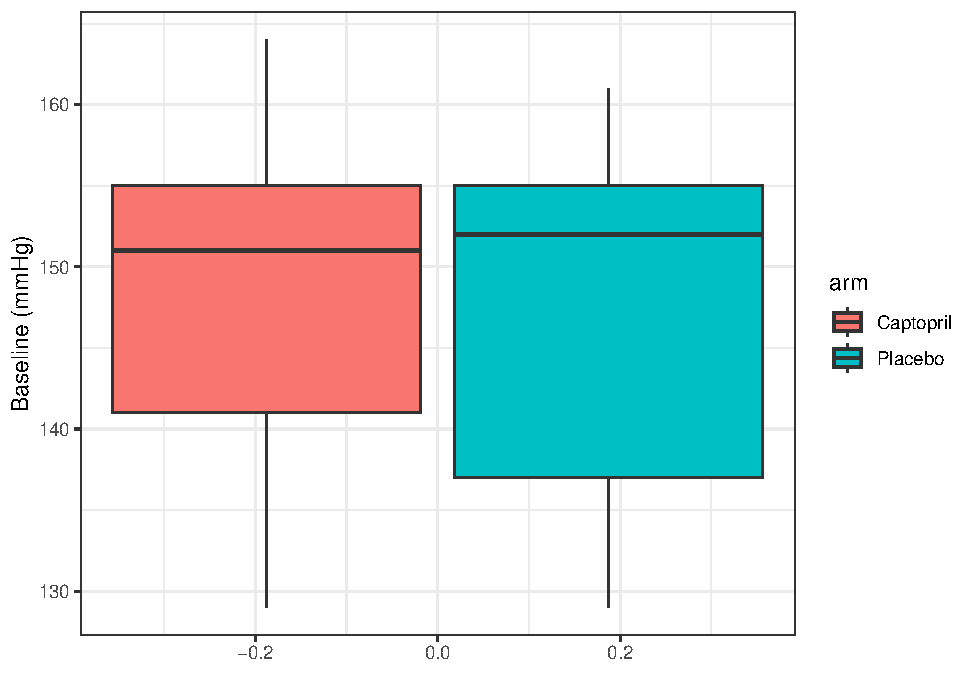
\includegraphics{CT4H_notes_files/figure-latex/hommel-1.pdf}
\caption{\label{fig:hommel}Baseline measurements from the Captopril trial.}
\end{figure}

The baseline measurements are not identical in each group. Indeed, we saw earlier that the means differ by 1.4 mmHg. Although this isn't a clinically significant difference, or a large enough difference to make us doubt the randomisation procedure, it is still a difference.

The basic principle of ANCOVA is that if there is some correlation between the baseline and outcome measurements, then if the baseline measurements differ, one would expect the outcome measurements to differ, even if there is no treatment effect (ie. if \(\tau=0\)). Indeed, how do we decide how much of the difference in outcome is down to the treatment itself, and how much is simply the difference arising from different samples?

This issue arises in many trials, particularly where there is a strong correlation between baseline and outcome measurements.

\hypertarget{ancovatheory}{%
\subsection{The theory}\label{ancovatheory}}

Suppose the outcome for a clinical trial is \(X\) and the baseline is \(B\). \(X\) has mean \(\mu\) in the control group (C) and mean \(\mu+\tau\) in the test group (T), and as usual our aim is to determine the extent of \(\tau\), the treatment effect. We suppose also that \(X\) has variance \(\sigma^2\) in both groups.

The same quantity is measured at the start of the trial, and this is the baseline \(B\), which we can assume to have true mean \(\mu_B\) in both groups (because of randomisation) and variance \(\sigma^2\). We also assume that the true correlation between \(B\) and \(X\) is \(\rho\) in each group. Finally, we assume that both treatment groups are of size \(N\).

We therefore have \(2N\) patients, and so we observe baseline measurements \(b_1,\,b_2,\ldots,b_{2N}\). Given these values, we have

\[
\begin{aligned}
\operatorname{E}\left(X_i\mid{b_i}\right) &= \mu + \rho\left(b_i - \mu_B\right)\text{ in the control group}\\
\operatorname{E}\left(X_i\mid{b_i}\right) &= \mu +\tau + \rho\left(b_i - \mu_B\right)\text{ in the test group.}
\end{aligned}
\]

From this, we find that

\begin{equation}
\operatorname{E}\left(\bar{X}_T - \bar{X}_C\mid{\bar{b}_T,\,\bar{b}_C}\right) = \tau + \rho\left(\bar{b}_T - \bar{b}_C\right). 
\label{eq:diffexp}
\end{equation}
That is, if there is a difference in the baseline mean between the control and test groups, then the difference in outcome means is not an unbiased estimator of the treatment effect \(\tau\). Assuming \(\rho>0\) (which is almost always the case) then if \(\bar{b}_T>\bar{b}_C\) the difference in outcome means overestimates \(\tau\). Conversely, if \(\bar{b}_T<\bar{b}_C\), the difference in outcome means underestimates \(\tau\). The only situation in which the difference in outcome means is an unbiased estimator is when \(\rho=0\), however this is not common in practice.

Comparing the difference between outcome and baseline, as we did in \ref{baseline}, does not solve this problem, since we have

\[\operatorname{E}\left[\left(\bar{X}_T - \bar{b}_T\right) - \left(\bar{X}_C - \bar{b}_C\right)\mid{\bar{b}_T,\,\bar{b}_C}\right] = \tau + \left(\rho-1\right)\left(\bar{b}_T - \bar{b}_C\right),\]
which is similarly biased (unless \(\rho=1\), which is never the case).

Notice, however, that if we use as our estimator

\begin{equation}
\hat{\tau} = \left(\bar{X}_T - \bar{X}_C\right) - \rho \left(\bar{b}_T - \bar{b}_C\right)
\label{eq:ancovaest}
\end{equation}

then, following from Equation \eqref{eq:diffexp} we have

\[
\operatorname{E}\left[\left(\bar{X}_T - \bar{X}_C\right) - \rho \left(\bar{b}_T - \bar{b}_C\right)\mid{\bar{b}_T,\,\bar{b}_C}\right] = \tau + \rho\left(\bar{b}_T - \bar{b}_C\right)- \rho\left(\bar{b}_T - \bar{b}_C\right) = \tau. \]

\hypertarget{whats-the-variance-of-this-estimator}{%
\subsubsection{What's the variance of this estimator?}\label{whats-the-variance-of-this-estimator}}

To work out the variance of \(\hat{\tau}\) in Equation \eqref{eq:ancovaest} we need to think about bivariate normal variables.

Let's suppose that random variables \(X\) and \(Y\) are jointly normally distributed with correlation \(\rho\)

\begin{equation}
\begin{pmatrix}
X\\
Y
\end{pmatrix} \sim N\left(
\begin{pmatrix}
\mu_X\\
\mu_Y
\end{pmatrix},\;
\begin{pmatrix}
\sigma^2_X & \rho\sigma_X\sigma_Y \\
\rho\sigma_X\sigma_Y & \sigma^2_Y
\end{pmatrix}
\right).
\label{eq:bvn}
\end{equation}

From Equation \eqref{eq:bvn}, we know that \(\operatorname{E}\left(Y\right) = \mu_Y\).

But, if we have observed \(X=x\), this gives us some information about likely values of \(Y\): if \(\rho>0\) then a lower value of \(x\) should lead us to expect a lower value of \(Y\), for example. Figure \ref{fig:bvnplot} shows

\begin{equation}
\begin{pmatrix}
X\\
Y
\end{pmatrix} \sim N\left(
\begin{pmatrix}
0\\
0
\end{pmatrix},\;
\begin{pmatrix}
2 & 1.5 \\
1.5 & 3
\end{pmatrix}
\right).
\label{eq:bvneg}
\end{equation}

\begin{figure}
\centering
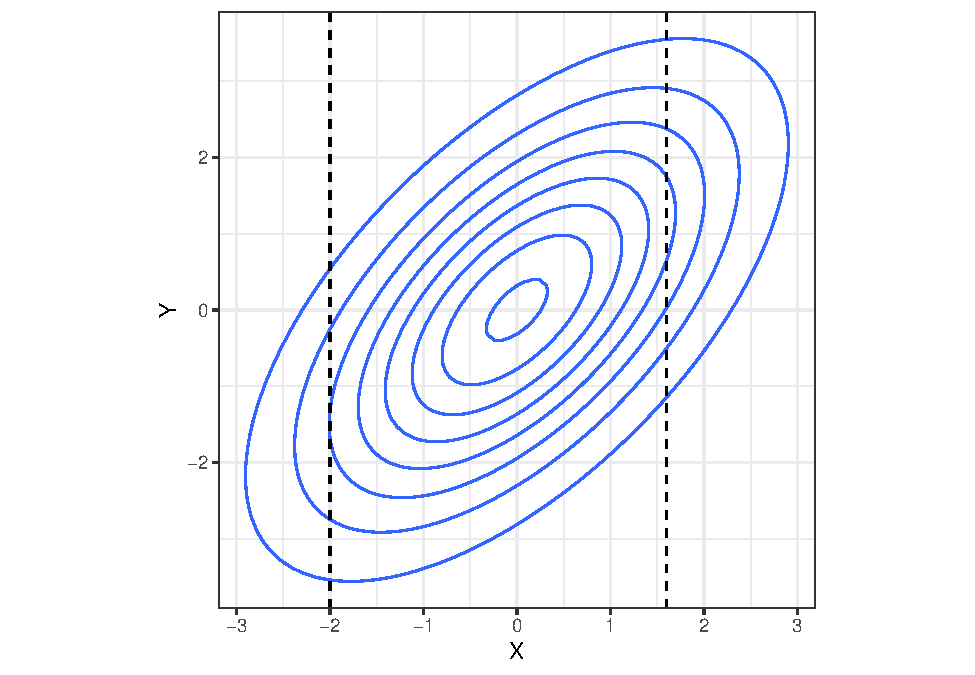
\includegraphics{CT4H_notes_files/figure-latex/bvnplot-1.pdf}
\caption{\label{fig:bvnplot}A bivariate normal density.}
\end{figure}

The higher the value of \(\rho\) (in magnitude), the more the conditional distribution of \(Y\) given an observed value of \(x\) deviates from the marginal distribution of \(Y\) (in our example, \(N\left(0,\;3\right)\)). In particular, \[\operatorname{E}\left(Y\mid{X=x}\right)\neq{\operatorname{E}\left(Y\right)}.\]

If we have another random variable, \(W\), that is independent of \(Y\) (and note that if two normally distributed variables are uncorrelated, they are also independent), then observing \(W=w\) doens't give us any information about the distribution of \(Y\), so we have

\[ \operatorname{E}\left(Y\mid{W=w}\right)={\operatorname{E}\left(Y\right)}. \]
We can combine this information to work out \(\operatorname{E}\left(Y\mid{X=x}\right)\). Firstly, we'll calculate the covariance of \(X\) and \(Y-kX\), for some constant \(k\). We can find this by

\[
\begin{aligned}
\operatorname{cov}\left(X,\,Y-kX\right) &= \operatorname{E}\left[\left(X-\mu_X\right)\left(Y-kX - \mu_Y + k\mu_X\right)\right]\\
&\text{ (using that }\operatorname{cov\left(X,Y\right)=\operatorname{E}\left[\left(X-\operatorname{E}\left(X\right)\right)\left(Y-\operatorname{E}\left(Y\right)\right)\right]}\\
& = \operatorname{E}\left[\left(X-\mu_X\right)\left(Y-\mu_Y\right) - k\left(X-\mu_X\right)^2\right]\\
& = \rho \sigma_X\sigma_Y - k\sigma_X^2.
\end{aligned}
\]
If we set

\[k = \beta = \frac{\rho\sigma_Y}{\sigma_X} \]
then \(\operatorname{cov}\left(X,\,Y-\beta X\right)=0\), and since \(Y-\beta X\) is also normally distributed, this means that \(X\) and \(Y-\beta X\) are independent. Therefore we have

\[\operatorname{E}\left(Y-\beta X \mid X=x\right) = \operatorname{E}\left(Y-\beta X\right) = \mu_Y - \beta \mu_X.\]
However, since we're conditioning on an observed value of \(X=x\) we can take \(X\) to be fixed at this value, and so \(\operatorname{E}\left(\beta X\mid{X=x}\right) = \beta x\). Finally, this allows us to calculate

\[
\begin{aligned}
\operatorname{E}\left(Y\mid{X=x}\right) & = \operatorname{E}\left(\beta X\mid{X=x}\right) + \mu_Y - \beta\mu_X\\
& = \mu_Y + \beta\left(x - \mu_X\right).
\end{aligned}
\]

We can use the same idea to find \(\operatorname{var}\left(Y\mid{X=x}\right)\).

Recall that \(\operatorname{var}\left(Y\right) = \operatorname{E}\left[Y^2\right] - \left[\operatorname{E}\left(Y\right)\right]^2\), and so

\begin{equation}
\operatorname{var}\left(Y\mid{X=x}\right) = \operatorname{E}\left(Y^2\mid{X=x}\right) - \left[\operatorname{E}\left(Y\mid{X=x}\right)\right]^2. 
\label{eq:vary2}
\end{equation}

We already know the second term, and we can find the first term using the same idea as before, this time noting that \(X\) and \(\left(Y-\beta X\right)^2\) are independent.

From this, and using the fact that (for example)

\[
\begin{aligned}
\operatorname{var}\left(X\right) & = \operatorname{E}\left(X^2\right) - \left[\operatorname{E}\left(X\right)\right]^2\\
\text{and therefore} & \\
\operatorname{E}\left(X^2\right)  &= \sigma_X^2 + \mu_X^2,
\end{aligned}
\]

we find that

\begin{equation}
\operatorname{E}\left[\left(Y-\beta X\right)^2 \mid X=x\right] = \operatorname{E}\left[\left(Y-\beta X\right)^2\right] =S^2 + \left(\mu_Y - \beta \mu_X\right)^2,
\label{eq:evary1}
\end{equation}

where \(S^2 = \sigma^2_Y + \beta^2\sigma^2_X - 2\beta\rho\sigma_X\sigma_Y = \sigma^2_Y\left(1-\rho^2\right)\) (by plugging in \(\beta = \frac{\rho\sigma_Y}{\sigma_X}\)).

If we multiply out the left-hand side of Equation \eqref{eq:evary1}, we find that this is the same as

\[\operatorname{E}\left[Y^2\mid{X=x}\right] - 2\beta\operatorname{E}\left(Y\mid{X=x}\right) + \beta^2 x^2 = \operatorname{E}\left[Y^2\mid{X=x}\right] - 2\beta x\left(\mu_Y - \beta\mu_X\right) - \beta^2 x^2.\]
Equating this with Equation \eqref{eq:evary1} and rearranging, we find

\[\operatorname{E}\left[Y^2\mid{X=x}\right] = S^2 + \left(\mu_Y - \beta\mu_X\right)^2 + 2\beta x\left(\mu_Y - \beta \mu_X\right) + \beta^2x^2.\]
Now we can expand out
\[\operatorname{E}\left(Y\mid{X=x}\right) = \mu_Y + \beta\left(x-\mu_X\right) = \left(\mu_Y - \beta\mu_X\right) +\beta x\]
to find

\[\left[\operatorname{E}\left(Y\mid{X=x}\right) \right]^2  = \left(\mu_Y - \beta\mu_X\right)^2 + 2\beta x \left(\mu_Y - \beta\mu_X\right) + \beta^2 x^2.\]
Finally (!) we can use these two expressions to find

\[
\begin{aligned}
\operatorname{var}\left(Y\mid{X=x}\right) & = \operatorname{E}\left[Y^2\mid{X=x}\right] - \left[\operatorname{E}\left(Y\mid{X=x}\right)\right]^2\\
& = S^2 \\
& = \sigma_Y^2\left(1-\rho^2\right).
\end{aligned}
\]
One thing to notice is that this conditional variance of doesn't depend on the observed value of \(X=x\). It can also never exceed \(\sigma^2_Y\), and is only equal to \(\sigma^2_Y\) if \(X\) and \(Y\) are uncorrelated.

\hypertarget{back-to-our-estimator}{%
\subsubsection*{Back to our estimator!}\label{back-to-our-estimator}}
\addcontentsline{toc}{subsubsection}{Back to our estimator!}

Recall that in ANCOVA our estimator of the treatment effect \(\tau\) is

\[ \hat{\tau} = \left(\bar{X}_T - \bar{X}_C\right) - \rho\left(\bar{b}_T - \bar{b}_C\right)\]
and that we have

\[\operatorname{cor}\left(\bar{X}_T - \bar{X}_C,\; \bar{b}_T - \bar{b}_C\right) = \rho.\]
Therefore, using the result we just found,

\[
\begin{aligned}
\operatorname{var}\left(\hat{\tau}\right) = \operatorname{var}\left[\left(\bar{X}_T - \bar{X}_C\right) - \rho\left(\bar{b}_T - \bar{b}_C\right)\mid{\bar{b}_T,\bar{b}_C}\right] &= \operatorname{var}\left[\left(\bar{X}_T - \bar{X}_C\right) \mid{\bar{b}_T,\bar{b}_C}\right]\\
& = \operatorname{var}\left(\bar{X}_T - \bar{X}_C\right)\left(1-\rho^2\right)\\
& = \frac{2\sigma^2}{N}\left(1-\rho^2\right).
\end{aligned}
\]
Notice that unlike our first estimator that used baseline values, in Section \ref{baseline}, the variance of the ANCOVA estimate can never exceed \(\frac{2\sigma^2}{N}\); if the baseline and outcome are uncorrelated, ANCOVA will perform as well as a \(t\)-test.

\citet{borm2007simple} discuss how this reduction in \(\operatorname{var\left(\hat{\tau}\right)}\) can impact our sample size calculations.

\hypertarget{the-practice}{%
\subsection{The practice}\label{the-practice}}

In the previous section we established an unbiased estimate of the treatment effect that takes into account the baseline measurements. However, we can't use it as a model, because there are a few practical barriers:

\begin{itemize}
\tightlist
\item
  Our estimate for \(\tau\) relies on the correlation \(\rho\), which is unknown
\item
  In real life, the groups are unlikely to have equal size and variance, so ideally we'd lose these constraints
\end{itemize}

We can solve both of these by fitting the following statistical model to the observed outcomes \(x_i\):

\[
\begin{aligned}
x_i & = \mu + \gamma b_i + \epsilon_i & \text{ in group C}\\
x_i & = \mu + \tau + \gamma b_i + \epsilon_i & \text{ in group T}&.
\end{aligned}
\]
Here, the \(\epsilon_i\) are independent errors with distribution \(N\left(0,\,\sigma^2\right)\), the \(b_i\) are the baseline measurements for \(i=1,\ldots,N_T+N_C\), for groups \(T\) and \(C\) with sizes \(N_T\) and \(N_C\) respectively. Sometimes this is written instead in the form

\[ x_i = \mu + \tau G_i+ \gamma b_i + \epsilon_i \]
where \(G_i\) is 1 if participant \(i\) is in group \(T\) and 0 if they're in group \(C\). This is a factor variable, which you may remember from Stats Modelling II (if you took it). If \(G_i=1\) (ie. participant \(i\) is in group \(T\)) then \(\tau\) is added. If \(G_i=0\) (ie. participant \(i\) is in group \(C\)) then it isn't.

We now have four parameters to estimate: \(\mu,\,\tau,\,\gamma\) and \(\sigma^2\). For the first three we can use least squares (as you have probably seen for linear regression). Our aim is to minimise the sum of squares

\[S\left(\mu,\, \tau,\,\gamma\right) = \sum\limits_{i\text{ in }T} \left(x_i - \mu - \tau - \gamma b_i\right)^2 + \sum\limits_{i\text{ in }C} \left(x_i - \mu - \gamma b_i\right)^2.\]

This leads to estimates \(\hat{\mu},\, \hat{\tau}\) and \(\hat{\gamma}\). We won't worry about how this sum is minimised, since we'll always be using pre-written R functions. We can use the estimates \(\hat{\mu},\, \hat{\tau}\) and \(\hat{\gamma}\) to estimate \(\sigma^2\), using

\[\hat{\sigma}^2 = \frac{S\left(\hat{\mu},\hat{\tau}, \hat{\gamma}\right)}{N_T + N_C -3}.\]
The general form for this is

\[ \hat{\sigma}^2 = \frac{SSE}{n-p},\]
where \(SSE\) is the residual sum of squares, \(n\) is the number of data points and \(p\) the number of parameters (apart from \(\sigma^2\)) being estimated. If you want to know why that is, you can find out \href{https://pages.stern.nyu.edu/~wgreene/MathStat/GreeneChapter4.pdf}{here} (look particularly at page 62), but we will just take it as given!

As well as generating a fitted value \(\hat{\tau}\), we (or rather R!) will also find the standard error of \(\hat\tau\), and we can use this to generate a confidence interval for the treatment effect \(\tau\).

The technique described above is a well-established statistical method known as \textbf{ANCOVA} (short for the \textbf{An}alysis of \textbf{Cova}riance), which can be implemented in R and many other statistical software packages. Notice that it is really just a linear model (the like of which you have seen many times) with at least one factor variable, and with a particular focus (application-wise) on the coefficient of the treatment group variable.

\begin{example}
Let's now implement ANCOVA on our Captopril data in R.
We do this by first fitting a linear model using `lm', with baseline measurement and arm as predictor variables and outcome as the predictand.

\begin{Shaded}
\begin{Highlighting}[]
\NormalTok{lm\_capt }\OtherTok{=} \FunctionTok{lm}\NormalTok{(outcome }\SpecialCharTok{\textasciitilde{}}\NormalTok{ baseline }\SpecialCharTok{+}\NormalTok{ arm, }\AttributeTok{data =}\NormalTok{ df\_hommel)}
\FunctionTok{summary}\NormalTok{(lm\_capt)}
\end{Highlighting}
\end{Shaded}

\begin{verbatim}
## 
## Call:
## lm(formula = outcome ~ baseline + arm, data = df_hommel)
## 
## Residuals:
##    Min     1Q Median     3Q    Max 
## -9.129 -3.445  1.415  2.959 11.076 
## 
## Coefficients:
##             Estimate Std. Error t value Pr(>|t|)   
## (Intercept)  67.5731    19.7577   3.420  0.00456 **
## baseline      0.4578     0.1328   3.446  0.00434 **
## armPlacebo    7.1779     2.9636   2.422  0.03079 * 
## ---
## Signif. codes:  0 '***' 0.001 '**' 0.01 '*' 0.05 '.' 0.1 ' ' 1
## 
## Residual standard error: 5.869 on 13 degrees of freedom
## Multiple R-squared:  0.5629, Adjusted R-squared:  0.4957 
## F-statistic: 8.372 on 2 and 13 DF,  p-value: 0.004608
\end{verbatim}

The variable `arm' here is being included as a factor variable, so it behaves like

\[
\text{arm}_i =
\begin{cases}
0 & \text{ if participant }i\text{ is assigned Captopril}\\
1 & \text{ if participant }i\text{ is assigned Placebo}.
\end{cases}
\]
Therefore, for a patient assigned Placebo, a value of 7.1779 is added, as well as the intercept and baseline term. This results in a model with two parallel fitted lines.

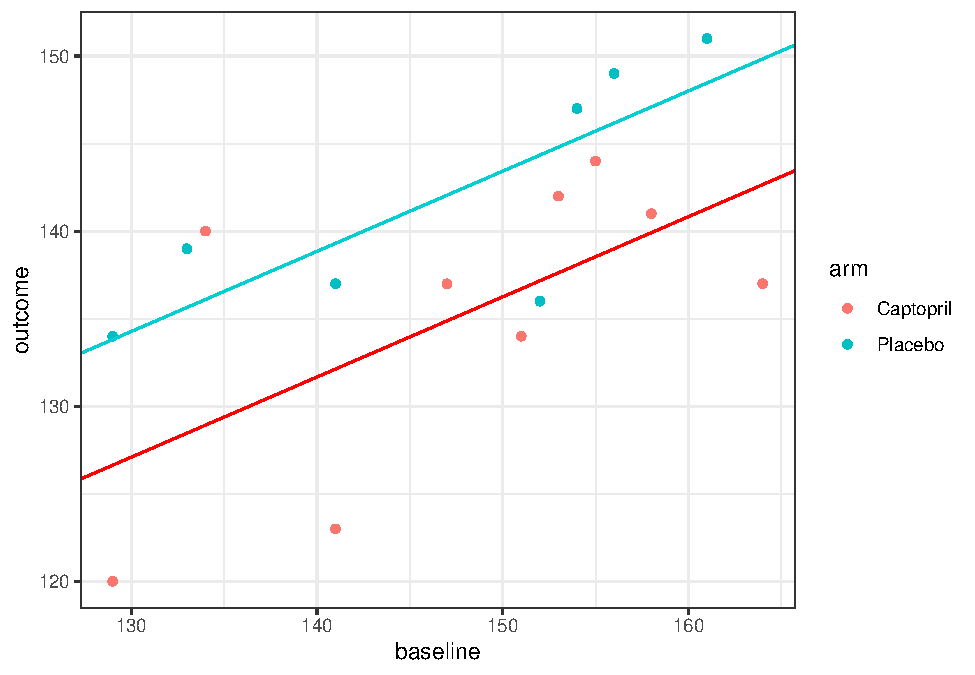
\includegraphics{CT4H_notes_files/figure-latex/unnamed-chunk-14-1.pdf}

For our previous methods we have calculated a confidence interval for the treatment effect \(\tau\), and we will do that here too. The second column of the linear model summary (above) gives the standard errors of each estimated parameter, and we see that the standard error of \(\hat{\tau}\) is 2.9636. Therefore, to construct a 95/\% confidence interval for \(\hat{\tau}\), we use (to 3 decimal places)

\(7.178\; \pm\; t_{0.975;13}\times{2.964} = \left(0.775,\; 13.580\right).\)

The model has \(n-p=13\) degrees of freedom because there are \(n=16\) data points and we are estimating \(p=3\) parameters.
Notice that unlike our previous confidence intervals, this doesn't contain zero, and so our analysis has enabled us to conclude that there is a significant reduction in blood pressure with Captopril. You can also see this in that \(p=0.03079<0.05\). However, you can tell from the width of the interval (and the fact that \(p\) is still quite close to 0.05) that there is still a lot of uncertainty about \(\tau\).

The `Residual standard error' term near the bottom of the linear model summary is the estimate of \(\hat{\sigma}\), so here we have \(\hat{\sigma}^2 = 5.869^2 = 34.44.\)

As with any fitted model, we should check the residuals.

\begin{Shaded}
\begin{Highlighting}[]
\NormalTok{resid\_capt }\OtherTok{=} \FunctionTok{resid}\NormalTok{(lm\_capt)}
\NormalTok{df\_hommel}\SpecialCharTok{$}\NormalTok{resid}\OtherTok{=}\NormalTok{ resid\_capt}

\FunctionTok{ggplot}\NormalTok{(}\AttributeTok{data =}\NormalTok{ df\_hommel, }\FunctionTok{aes}\NormalTok{(}\AttributeTok{x=}\NormalTok{baseline, }\AttributeTok{y=}\NormalTok{resid, }\AttributeTok{col=}\NormalTok{arm)) }\SpecialCharTok{+} 
  \FunctionTok{geom\_point}\NormalTok{() }\SpecialCharTok{+}
  \FunctionTok{geom\_hline}\NormalTok{(}\AttributeTok{yintercept=}\DecValTok{0}\NormalTok{)}\SpecialCharTok{+}
  \FunctionTok{xlab}\NormalTok{(}\StringTok{"Baseline"}\NormalTok{)}\SpecialCharTok{+}
  \FunctionTok{ylab}\NormalTok{(}\StringTok{"Residual"}\NormalTok{)}\SpecialCharTok{+}\FunctionTok{theme\_bw}\NormalTok{()}
\end{Highlighting}
\end{Shaded}

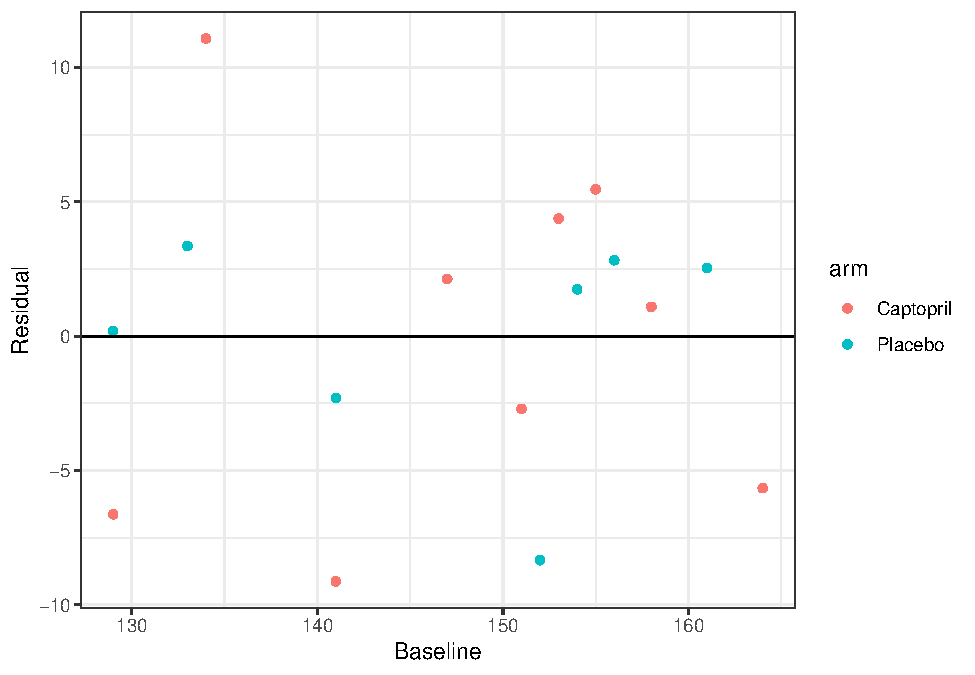
\includegraphics{CT4H_notes_files/figure-latex/unnamed-chunk-15-1.pdf}

These look pretty good; there are no clear patterns and the distribution appears to be similar for each treatment group. Though, with such a small sample it's difficult really to assess the fit of the model.
\end{example}

\hypertarget{some-follow-up-questions.}{%
\section{Some follow-up questions\ldots.}\label{some-follow-up-questions.}}

This might have raised a few questions, so we will address those now.

\hypertarget{didnt-we-say-that-x_t---x_c-was-an-unbiased-estimator-of-tau}{%
\subsection{\texorpdfstring{Didn't we say that \(X_T - X_C\) was an unbiased estimator of \(\tau\)?}{Didn't we say that X\_T - X\_C was an unbiased estimator of \textbackslash tau?}}\label{didnt-we-say-that-x_t---x_c-was-an-unbiased-estimator-of-tau}}

In Sections \ref{ttest} and \ref{baseline} we used both \(\bar{X}_T - \bar{X}_C\) and \(\left(\bar{X}_T - \bar{B}_T\right) - \left(\bar{X}_C - \bar{B}_C\right)\) as unbiased estimators of \(\tau\).
Then, in Section \ref{ancovatheory} we showed that

\[
\begin{aligned}
\operatorname{E}\left(\bar{X}_T - \bar{X}_C\mid{\bar{b}_T,\;\bar{b}_C}\right)& = \tau + \rho\left(\bar{b}_T - \bar{b}_C\right)\\
\operatorname{E}\left[\left(\bar{X}_T - \bar{b}_T\right) - \left(\bar{X}_C - \bar{b}_C\right)\mid{\bar{b}_T,\,\bar{b}_C}\right] &= \tau + \left(\rho-1\right)\left(\bar{b}_T - \bar{b}_C\right),
\end{aligned}
\]
that is, neither of these quantities are unbiased estimators of \(\tau\) (except in very specific circumstances).

Is this a contradiction?

You'll be relieved to hear (and may already have realised) that it isn't; the first pair of equations are blind to the baseline values \(B_T\) and \(B_C\), and are using their statistical properties. Because of the randomisation procedure, a priori they can be treated the same. However, once we have observed values for the baseline, \(b_T\) and \(b_C\), they are very unlikely to be exactly the same. They are also (along with all other baseline measurements, often things like age, sex, height etc.) definitely not affected by the trial, since they are taken before any placebo or treatment has been administered, and often even before allocation. However, conditioning on their observed values can reduce the variance of our estimate of \(\tau\), as we have seen.

In this sense, the observed baseline means \(\bar{b}_T\) and \(\bar{b}_C\) are known as \textbf{ancillary statistics}; they contain no direct information about the parameter we are interested in (in this case the treatment effect \(\tau\)), but our inferences can be improved by conditioning on the observed values of the ancillary statistics.

\hypertarget{what-if-the-lines-shouldnt-be-parallel-the-unequal-slopes-model}{%
\subsection{What if the lines shouldn't be parallel? The unequal slopes model}\label{what-if-the-lines-shouldnt-be-parallel-the-unequal-slopes-model}}

In the analysis above, we have assumed that the coefficient \(\gamma\) of baseline (the estimate of the correlation between outcome and baseline) is the same in both groups; we have fitted an \textbf{equal slopes model}. It isn't obvious that this should be the case, and indeed we can test for it.

Allowing each group to have a different slope means including an interaction term between baseline and treatment group,

\[ x_i = \mu + \tau G_i+ \gamma b_i + \lambda b_i G_i + \epsilon_i . \]
The term \(\lambda b_i G_i\) is 0 if participant \(i\) is in group \(C\) and \(\lambda b_i\) if participant \(i\) is in group \(T\). Therefore, for participants in group \(C\), the gradient is still \(\gamma\), but for participants in group \(T\) it is now \(\gamma + \lambda\). We can test whether this interaction term should be included (that is, whether we should fit an unequal slopes model) by including it in a model and analysing the results.

\begin{example}
Continuing once again with the Captopril dataset, we now fit the model

\begin{Shaded}
\begin{Highlighting}[]
\NormalTok{lm\_capt\_int }\OtherTok{=} \FunctionTok{lm}\NormalTok{(outcome }\SpecialCharTok{\textasciitilde{}}\NormalTok{ arm }\SpecialCharTok{+}\NormalTok{ baseline }\SpecialCharTok{+}\NormalTok{ baseline}\SpecialCharTok{:}\NormalTok{arm, }\AttributeTok{data =}\NormalTok{ df\_hommel)}
\FunctionTok{summary}\NormalTok{(lm\_capt\_int)}
\end{Highlighting}
\end{Shaded}

\begin{verbatim}
## 
## Call:
## lm(formula = outcome ~ arm + baseline + baseline:arm, data = df_hommel)
## 
## Residuals:
##    Min     1Q Median     3Q    Max 
## -9.094 -3.475  1.412  2.979 11.145 
## 
## Coefficients:
##                     Estimate Std. Error t value Pr(>|t|)  
## (Intercept)         66.85150   28.02488   2.385   0.0344 *
## armPlacebo           8.72484   40.93465   0.213   0.8348  
## baseline             0.46272    0.18886   2.450   0.0306 *
## armPlacebo:baseline -0.01051    0.27723  -0.038   0.9704  
## ---
## Signif. codes:  0 '***' 0.001 '**' 0.01 '*' 0.05 '.' 0.1 ' ' 1
## 
## Residual standard error: 6.108 on 12 degrees of freedom
## Multiple R-squared:  0.563,  Adjusted R-squared:  0.4537 
## F-statistic: 5.153 on 3 and 12 DF,  p-value: 0.01614
\end{verbatim}

We see that the \(p\)-value for the coefficient \(\lambda\) (seen in the \texttt{arm:baseline} row) is not at all significant (0.97). Therefore we can be confident that there is no need to fit unequal slopes for this dataset. This fits with our earlier conclusion (from inspecting the residuals) that just including first order terms is fine.
\end{example}

\hypertarget{can-we-include-any-other-baseline-covariates}{%
\subsection{Can we include any other baseline covariates?}\label{can-we-include-any-other-baseline-covariates}}

In Section \ref{baseline} when our estimated treatment effect was \(\hat\tau = \left(\bar{x}_T - \bar{b}_T\right) - \left(\bar{x}_C - \bar{b}_C\right)\), the only other variable we could take into account was the baseline measurement, because it is on the same scale as the outcome \(X\). However, in ANCOVA, our treatment effect is

\[ \hat\tau = \left(\bar{x}_T - \bar{x}_C\right) - \hat\gamma\left(\bar{b}_T - \bar{b}_C\right), \]
and the inclusion of the coefficient \(\gamma\) means that we can include other covariates on different scales too. The key issue is that we can only include as covariates things that were already known before allocation (hence they are sometimes known as \emph{baseline covariates}, not to be confused with `the baseline', which would generally mean the same measurement as the primary outcome, but before treatment). This is because they cannot, at that point, have been affected by the treatment, or have had an influence on the post-trial outcome measurement. Indeed, as a rule, any variable that was used in the randomisation procedure (this particularly applies to minimisation and stratified sampling) should be included in the analysis.

\begin{example}
The data for this example is taken from \citet{datarium}. In this study, 60 patients take part in a trial investigating the effect of a new treatment and exercise on their stress score, after adjusting for age.
There are two treatment levels (yes or no) and three exercise levels (low, moderate and high) and 10 participants for each combination of treatment and exercise levels. Because in ANCOVA we fit a coefficient to every covariate, we can include exercise (another factor variable) and age (a continuous variable) in this analysis.

\begin{tabular}{r|r|l|l|r}
\hline
id & score & treatment & exercise & age\\
\hline
1 & 95.6 & yes & low & 59\\
\hline
2 & 82.2 & yes & low & 65\\
\hline
3 & 97.2 & yes & low & 70\\
\hline
4 & 96.4 & yes & low & 66\\
\hline
5 & 81.4 & yes & low & 61\\
\hline
6 & 83.6 & yes & low & 65\\
\hline
7 & 89.4 & yes & low & 57\\
\hline
8 & 83.8 & yes & low & 61\\
\hline
9 & 83.3 & yes & low & 58\\
\hline
10 & 85.7 & yes & low & 55\\
\hline
11 & 97.2 & yes & moderate & 62\\
\hline
12 & 78.2 & yes & moderate & 61\\
\hline
13 & 78.9 & yes & moderate & 60\\
\hline
14 & 91.8 & yes & moderate & 59\\
\hline
15 & 86.9 & yes & moderate & 55\\
\hline
16 & 84.1 & yes & moderate & 57\\
\hline
17 & 88.6 & yes & moderate & 60\\
\hline
18 & 89.8 & yes & moderate & 63\\
\hline
19 & 87.3 & yes & moderate & 62\\
\hline
20 & 85.4 & yes & moderate & 57\\
\hline
21 & 81.8 & yes & high & 58\\
\hline
22 & 65.8 & yes & high & 56\\
\hline
23 & 68.1 & yes & high & 57\\
\hline
24 & 70.0 & yes & high & 59\\
\hline
25 & 69.9 & yes & high & 59\\
\hline
26 & 75.1 & yes & high & 60\\
\hline
27 & 72.3 & yes & high & 55\\
\hline
28 & 70.9 & yes & high & 53\\
\hline
29 & 71.5 & yes & high & 55\\
\hline
30 & 72.5 & yes & high & 58\\
\hline
31 & 84.9 & no & low & 68\\
\hline
32 & 96.1 & no & low & 62\\
\hline
33 & 94.6 & no & low & 61\\
\hline
34 & 82.5 & no & low & 54\\
\hline
35 & 90.7 & no & low & 59\\
\hline
36 & 87.0 & no & low & 63\\
\hline
37 & 86.8 & no & low & 60\\
\hline
38 & 93.3 & no & low & 67\\
\hline
39 & 87.6 & no & low & 60\\
\hline
40 & 92.4 & no & low & 67\\
\hline
41 & 100.0 & no & moderate & 75\\
\hline
42 & 80.5 & no & moderate & 54\\
\hline
43 & 92.9 & no & moderate & 57\\
\hline
44 & 84.0 & no & moderate & 62\\
\hline
45 & 88.4 & no & moderate & 65\\
\hline
46 & 91.1 & no & moderate & 60\\
\hline
47 & 85.7 & no & moderate & 58\\
\hline
48 & 91.3 & no & moderate & 61\\
\hline
49 & 92.3 & no & moderate & 65\\
\hline
50 & 87.9 & no & moderate & 57\\
\hline
51 & 91.7 & no & high & 56\\
\hline
52 & 88.6 & no & high & 58\\
\hline
53 & 75.8 & no & high & 58\\
\hline
54 & 75.7 & no & high & 58\\
\hline
55 & 75.3 & no & high & 52\\
\hline
56 & 82.4 & no & high & 53\\
\hline
57 & 80.1 & no & high & 60\\
\hline
58 & 86.0 & no & high & 62\\
\hline
59 & 81.8 & no & high & 61\\
\hline
60 & 82.5 & no & high & 61\\
\hline
\end{tabular}

Table \ref{tab:sumstress} shows the mean and standard deviation of age for each combination of treatment and exercise level. If we were being picky / thorough, we might note that (perhaps unsurprisingly!) the mean and standard deviation of age are both lower in the high exercise groups. This might well affect our analysis, but we won't go into this now.

\begin{table}

\caption{\label{tab:sumstress}Summary of the stress dataset}
\centering
\begin{tabular}[t]{l|l|r|r}
\hline
Treatment & Exercise & Mean age & SD age\\
\hline
yes & low & 61.7 & 4.691600\\
\hline
yes & moderate & 59.6 & 2.590581\\
\hline
yes & high & 57.0 & 2.211083\\
\hline
no & low & 62.1 & 4.332051\\
\hline
no & moderate & 61.4 & 5.947922\\
\hline
no & high & 57.9 & 3.381321\\
\hline
\end{tabular}
\end{table}

Fitting a linear model, we see that treatment, high levels of exercise and age each have a significant effect on stress.

\begin{Shaded}
\begin{Highlighting}[]
\NormalTok{lm\_stresslin }\OtherTok{=} \FunctionTok{lm}\NormalTok{(score }\SpecialCharTok{\textasciitilde{}}\NormalTok{ treatment }\SpecialCharTok{+}\NormalTok{ exercise }\SpecialCharTok{+}\NormalTok{ age, }\AttributeTok{data =}\NormalTok{ stress)}
\FunctionTok{summary}\NormalTok{(lm\_stresslin)}
\end{Highlighting}
\end{Shaded}

\begin{verbatim}
## 
## Call:
## lm(formula = score ~ treatment + exercise + age, data = stress)
## 
## Residuals:
##     Min      1Q  Median      3Q     Max 
## -9.0261 -3.7497 -0.4285  3.0943 13.3696 
## 
## Coefficients:
##                  Estimate Std. Error t value Pr(>|t|)    
## (Intercept)      55.72934   10.91888   5.104 4.27e-06 ***
## treatmentno       4.32529    1.37744   3.140  0.00272 ** 
## exercisemoderate  0.08735    1.69032   0.052  0.95897    
## exercisehigh     -9.61841    1.84741  -5.206 2.96e-06 ***
## age               0.49811    0.17648   2.822  0.00662 ** 
## ---
## Signif. codes:  0 '***' 0.001 '**' 0.01 '*' 0.05 '.' 0.1 ' ' 1
## 
## Residual standard error: 5.288 on 55 degrees of freedom
## Multiple R-squared:  0.6045, Adjusted R-squared:  0.5757 
## F-statistic: 21.01 on 4 and 55 DF,  p-value: 1.473e-10
\end{verbatim}

In particular, taking a high level of exercise reduced participants' stress scores by around 9.6, and the treatment reduced stress scores by around 4.3. Participants' stress scores increased slightly with age (just under half a point per year!).

We can plot the residuals to check that the model is a reasonable fit

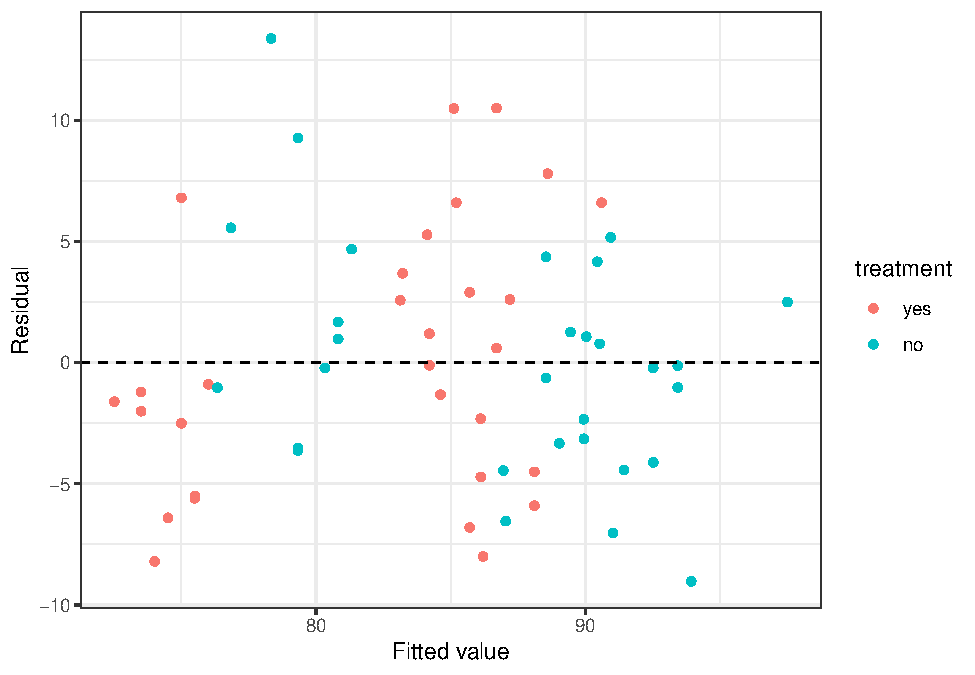
\includegraphics{CT4H_notes_files/figure-latex/unnamed-chunk-19-1.pdf}

And these look reasonably OK. We could also test for interactions, firstly across all factors:

\begin{verbatim}
## 
## Call:
## lm(formula = score ~ (treatment + exercise + age):(treatment + 
##     exercise + age), data = stress)
## 
## Residuals:
##     Min      1Q  Median      3Q     Max 
## -9.5637 -3.3982  0.4173  2.3827 10.3907 
## 
## Coefficients:
##                               Estimate Std. Error t value Pr(>|t|)   
## (Intercept)                   61.25416   19.86949   3.083  0.00333 **
## treatmentno                    3.89781   24.16324   0.161  0.87250   
## exercisemoderate             -14.60897   24.31690  -0.601  0.55070   
## exercisehigh                 -12.03441   29.53812  -0.407  0.68544   
## age                            0.43121    0.32097   1.343  0.18518   
## treatmentno:exercisemoderate  -0.20723    3.35949  -0.062  0.95106   
## treatmentno:exercisehigh       8.12783    3.72077   2.184  0.03365 * 
## treatmentno:age               -0.03769    0.38851  -0.097  0.92311   
## exercisemoderate:age           0.24286    0.40215   0.604  0.54864   
## exercisehigh:age              -0.03524    0.50722  -0.069  0.94488   
## ---
## Signif. codes:  0 '***' 0.001 '**' 0.01 '*' 0.05 '.' 0.1 ' ' 1
## 
## Residual standard error: 5.106 on 50 degrees of freedom
## Multiple R-squared:  0.6647, Adjusted R-squared:  0.6043 
## F-statistic: 11.01 on 9 and 50 DF,  p-value: 3.181e-09
\end{verbatim}

and then restricted to the interactions that seem important:

\begin{verbatim}
## 
## Call:
## lm(formula = score ~ treatment + exercise + age + treatment:exercise, 
##     data = stress)
## 
## Residuals:
##     Min      1Q  Median      3Q     Max 
## -9.3250 -3.0192  0.2745  2.4650 10.6667 
## 
## Coefficients:
##                               Estimate Std. Error t value Pr(>|t|)    
## (Intercept)                   56.79090   10.41383   5.453 1.32e-06 ***
## treatmentno                    1.52858    2.23026   0.685   0.4961    
## exercisemoderate               0.01746    2.25662   0.008   0.9939    
## exercisehigh                 -13.70331    2.36314  -5.799 3.78e-07 ***
## age                            0.50355    0.16684   3.018   0.0039 ** 
## treatmentno:exercisemoderate   0.15503    3.16129   0.049   0.9611    
## treatmentno:exercisehigh       8.21822    3.15375   2.606   0.0119 *  
## ---
## Signif. codes:  0 '***' 0.001 '**' 0.01 '*' 0.05 '.' 0.1 ' ' 1
## 
## Residual standard error: 4.985 on 53 degrees of freedom
## Multiple R-squared:  0.6613, Adjusted R-squared:  0.623 
## F-statistic: 17.25 on 6 and 53 DF,  p-value: 6.167e-11
\end{verbatim}

Notice that now, the effect of the treatment on its own is not significant. Also notice that for both the linear exercise terms and the interactions between the exercise and treatment, the effects of moderate and low exercise are very similar.
Combining the coefficients, someone who does a high level of exercise:

\begin{itemize}
\tightlist
\item
  is likely to reduce their stress score by 13.7 if they receive the treatment
\item
  is likely to reduce their stress score by \(13.7 - 8.2 = 5.5\) if they don't receive the treatment
\end{itemize}

Returning to our initial look at the dataset, the fact that age is a factor, and high levels of exercise are clearly very important should worry us slightly, since there are very few older people doing high levels of exercise. This may mean our model is inaccurate.
\end{example}

\hypertarget{an-important-caution}{%
\subsection*{An important caution!}\label{an-important-caution}}
\addcontentsline{toc}{subsection}{An important caution!}

As you'll have seen if you read \citet{kendall2003designing} (for formative assignment 1), we should have everything in place, including a statistical analysis plan, \textbf{before} the trial. We should already know which covariates we plan to include in our model, and how. `Trawling' for the best possible model by trying lots of different things (and inevitably settling on the one that leads to the most significant conclusion) is poor practice, and can increase the type I error rate (\(\alpha\)).

I realise that is sort of what we've done in this Section on Analysis, but that was to demonstrate and compare the different methods. Proceeding in the way we have, trying lots of different models, when analysing and writing up a trial would be very poor practice!

There's another excellent episode of the JAMA Evidence podcast, with a focus on adjusting for covariates, that talks about this issue (you can find it \href{https://edhub.ama-assn.org/jn-learning/audio-player/18836864}{here} and linked from Ultra).

That draws to a close our work with continuous outcome variables. In the next lecture, we'll start thinking about binary outcome variables.

\hypertarget{references}{%
\chapter*{References}\label{references}}
\addcontentsline{toc}{chapter}{References}

This sections lists the references used in the course - it will be updated as the notes are updated. Some of the more accessible (dare I say `interesting') resources are linked from the notes. If you want to read any of these articles, the easiest way is to copy the title into \href{https://scholar.google.co.uk/}{Google scholar}.

  \bibliography{ct4h.bib}

\end{document}
